\documentclass[]{article}
\usepackage{lmodern}
\usepackage{amssymb,amsmath}
\usepackage{ifxetex,ifluatex}
\usepackage{fixltx2e} % provides \textsubscript
\ifnum 0\ifxetex 1\fi\ifluatex 1\fi=0 % if pdftex
  \usepackage[T1]{fontenc}
  \usepackage[utf8]{inputenc}
\else % if luatex or xelatex
  \ifxetex
    \usepackage{mathspec}
  \else
    \usepackage{fontspec}
  \fi
  \defaultfontfeatures{Ligatures=TeX,Scale=MatchLowercase}
\fi
% use upquote if available, for straight quotes in verbatim environments
\IfFileExists{upquote.sty}{\usepackage{upquote}}{}
% use microtype if available
\IfFileExists{microtype.sty}{%
\usepackage{microtype}
\UseMicrotypeSet[protrusion]{basicmath} % disable protrusion for tt fonts
}{}
\usepackage[margin=1in]{geometry}
\usepackage{hyperref}
\hypersetup{unicode=true,
            pdftitle={The relationship between a translational cognitive measure of negative bias and self-reported psychiatric symptoms in a large online sample},
            pdfborder={0 0 0},
            breaklinks=true}
\urlstyle{same}  % don't use monospace font for urls
\usepackage{color}
\usepackage{fancyvrb}
\newcommand{\VerbBar}{|}
\newcommand{\VERB}{\Verb[commandchars=\\\{\}]}
\DefineVerbatimEnvironment{Highlighting}{Verbatim}{commandchars=\\\{\}}
% Add ',fontsize=\small' for more characters per line
\usepackage{framed}
\definecolor{shadecolor}{RGB}{248,248,248}
\newenvironment{Shaded}{\begin{snugshade}}{\end{snugshade}}
\newcommand{\KeywordTok}[1]{\textcolor[rgb]{0.13,0.29,0.53}{\textbf{#1}}}
\newcommand{\DataTypeTok}[1]{\textcolor[rgb]{0.13,0.29,0.53}{#1}}
\newcommand{\DecValTok}[1]{\textcolor[rgb]{0.00,0.00,0.81}{#1}}
\newcommand{\BaseNTok}[1]{\textcolor[rgb]{0.00,0.00,0.81}{#1}}
\newcommand{\FloatTok}[1]{\textcolor[rgb]{0.00,0.00,0.81}{#1}}
\newcommand{\ConstantTok}[1]{\textcolor[rgb]{0.00,0.00,0.00}{#1}}
\newcommand{\CharTok}[1]{\textcolor[rgb]{0.31,0.60,0.02}{#1}}
\newcommand{\SpecialCharTok}[1]{\textcolor[rgb]{0.00,0.00,0.00}{#1}}
\newcommand{\StringTok}[1]{\textcolor[rgb]{0.31,0.60,0.02}{#1}}
\newcommand{\VerbatimStringTok}[1]{\textcolor[rgb]{0.31,0.60,0.02}{#1}}
\newcommand{\SpecialStringTok}[1]{\textcolor[rgb]{0.31,0.60,0.02}{#1}}
\newcommand{\ImportTok}[1]{#1}
\newcommand{\CommentTok}[1]{\textcolor[rgb]{0.56,0.35,0.01}{\textit{#1}}}
\newcommand{\DocumentationTok}[1]{\textcolor[rgb]{0.56,0.35,0.01}{\textbf{\textit{#1}}}}
\newcommand{\AnnotationTok}[1]{\textcolor[rgb]{0.56,0.35,0.01}{\textbf{\textit{#1}}}}
\newcommand{\CommentVarTok}[1]{\textcolor[rgb]{0.56,0.35,0.01}{\textbf{\textit{#1}}}}
\newcommand{\OtherTok}[1]{\textcolor[rgb]{0.56,0.35,0.01}{#1}}
\newcommand{\FunctionTok}[1]{\textcolor[rgb]{0.00,0.00,0.00}{#1}}
\newcommand{\VariableTok}[1]{\textcolor[rgb]{0.00,0.00,0.00}{#1}}
\newcommand{\ControlFlowTok}[1]{\textcolor[rgb]{0.13,0.29,0.53}{\textbf{#1}}}
\newcommand{\OperatorTok}[1]{\textcolor[rgb]{0.81,0.36,0.00}{\textbf{#1}}}
\newcommand{\BuiltInTok}[1]{#1}
\newcommand{\ExtensionTok}[1]{#1}
\newcommand{\PreprocessorTok}[1]{\textcolor[rgb]{0.56,0.35,0.01}{\textit{#1}}}
\newcommand{\AttributeTok}[1]{\textcolor[rgb]{0.77,0.63,0.00}{#1}}
\newcommand{\RegionMarkerTok}[1]{#1}
\newcommand{\InformationTok}[1]{\textcolor[rgb]{0.56,0.35,0.01}{\textbf{\textit{#1}}}}
\newcommand{\WarningTok}[1]{\textcolor[rgb]{0.56,0.35,0.01}{\textbf{\textit{#1}}}}
\newcommand{\AlertTok}[1]{\textcolor[rgb]{0.94,0.16,0.16}{#1}}
\newcommand{\ErrorTok}[1]{\textcolor[rgb]{0.64,0.00,0.00}{\textbf{#1}}}
\newcommand{\NormalTok}[1]{#1}
\usepackage{longtable,booktabs}
\usepackage{graphicx,grffile}
\makeatletter
\def\maxwidth{\ifdim\Gin@nat@width>\linewidth\linewidth\else\Gin@nat@width\fi}
\def\maxheight{\ifdim\Gin@nat@height>\textheight\textheight\else\Gin@nat@height\fi}
\makeatother
% Scale images if necessary, so that they will not overflow the page
% margins by default, and it is still possible to overwrite the defaults
% using explicit options in \includegraphics[width, height, ...]{}
\setkeys{Gin}{width=\maxwidth,height=\maxheight,keepaspectratio}
\IfFileExists{parskip.sty}{%
\usepackage{parskip}
}{% else
\setlength{\parindent}{0pt}
\setlength{\parskip}{6pt plus 2pt minus 1pt}
}
\setlength{\emergencystretch}{3em}  % prevent overfull lines
\providecommand{\tightlist}{%
  \setlength{\itemsep}{0pt}\setlength{\parskip}{0pt}}
\setcounter{secnumdepth}{0}
% Redefines (sub)paragraphs to behave more like sections
\ifx\paragraph\undefined\else
\let\oldparagraph\paragraph
\renewcommand{\paragraph}[1]{\oldparagraph{#1}\mbox{}}
\fi
\ifx\subparagraph\undefined\else
\let\oldsubparagraph\subparagraph
\renewcommand{\subparagraph}[1]{\oldsubparagraph{#1}\mbox{}}
\fi

%%% Use protect on footnotes to avoid problems with footnotes in titles
\let\rmarkdownfootnote\footnote%
\def\footnote{\protect\rmarkdownfootnote}

%%% Change title format to be more compact
\usepackage{titling}

% Create subtitle command for use in maketitle
\newcommand{\subtitle}[1]{
  \posttitle{
    \begin{center}\large#1\end{center}
    }
}

\setlength{\droptitle}{-2em}

  \title{The relationship between a translational cognitive measure of negative
bias and self-reported psychiatric symptoms in a large online sample}
    \pretitle{\vspace{\droptitle}\centering\huge}
  \posttitle{\par}
    \author{}
    \preauthor{}\postauthor{}
    \date{}
    \predate{}\postdate{}
  

\begin{document}
\maketitle

\section{Background}\label{background}

This study builds on prior work developing a measure of negative
affective bias as indexed by proportion of mid tones interpreted as high
reward (`p(mid as high)') in A) a rat pharmacological model of mood and
anxiety disorders (Hales et al., 2016) and B) humans with mood and
anxiety disorders relative to healthy controls (Aylward et al., 2019).

\paragraph{Task details}\label{task-details}

In both cases, the 2-alternative-forced-choice task involved training
participants to press a button/lever (left or right) when they heard a
tone (high or low) to receive a reward (1 or 3 £/rat pellets). The
stimulus-response-outcome contingencies were 100\% (but counterbalanced
across individuals). Following training, participants were then also
played tones of a frequency exactly equidistant between the high and low
tones. The primary outcome of interest is the proportion of times the
participant pressed the button/lever associated with the high reward
outcome for the ambiguous mid tone (referred to as `p(mid as high)'). Of
note, the rat study is a within-subject anxiogenic manipulation, whereas
the human study is a case control design. Both A) symptomatic
(`Symptom') rats and B) humans both demonstrate significantly increased
negative affective bias (i.e.~reduced prediction that ambiguous outcomes
will lead to higher rewards: `p(mid as high)') relative to
non-symptomatic controls (`HC').

\paragraph{Next steps}\label{next-steps}

This prior work suggests that this cognitive measure is sensitive to
pathological symptoms. We have three objectives for the present study.
Firstly we wanted to explore and remove sources of between-subject bias
within the task so as to maximise our chances of measuring individual
differences in task performance. Secondly, we wanted to explore factors
which contribute to individual differences in task performance in a
large cross-sectional sample. Specifically, we are interested in which
specific psychiatric-relevant symptoms/traits contribute to task
performance. Finally, once we identify relevant traits, can we
re-capitulate the effect of clinical screening in a large unscreened
online sample?

\section{1: Piloting to explore sources of between-subject
bias}\label{piloting-to-explore-sources-of-between-subject-bias}

To speed up data collection and facilitate the collection of larger
samples we adapted the task for online use. To this end, we decided to
switch the task from the auditory domain (which would require us to
check/trust that remote participants could hear the stimuli) to the
visual domain. In the first pilot A) we tested N=264 participants in a
version of the task which substituted high and low frequency tones of
large and small area circles. This lead to four counterbalancing
versions (labelled 1-4 below; sorted by level of bias). Following
discovery of clear between-subject bias we next tested B) N=158
individuals on a task that involved orientation of a line. Instead of
high/low we had vertical/horizontal. The intermediate stimuli were
either 45 or 135 degrees, which lead to 8 counterbalancing versions
(labelled 1-8 below; sorted by level of bias).

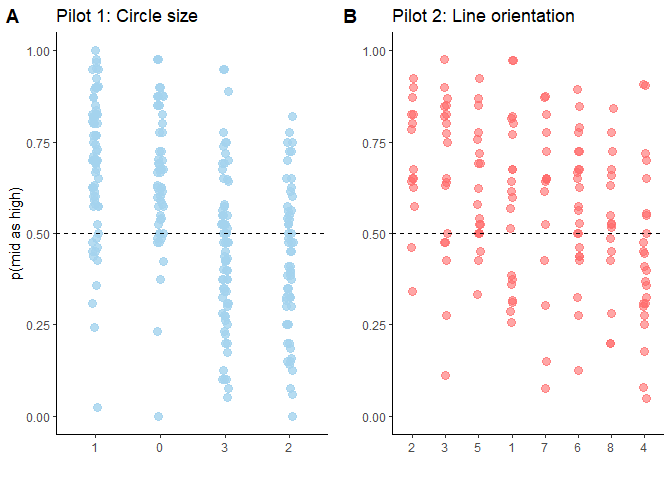
\includegraphics{OpenDataAnalysis_files/figure-latex/unnamed-chunk-3-1.pdf}

\begin{verbatim}
##              Df Sum Sq Mean Sq F value Pr(>F)    
## group         3  3.964  1.3215   35.28 <2e-16 ***
## Residuals   260  9.739  0.0375                   
## ---
## Signif. codes:  0 '***' 0.001 '**' 0.01 '*' 0.05 '.' 0.1 ' ' 1
\end{verbatim}

\begin{verbatim}
##          eta.sq eta.sq.part
## group 0.2893019   0.2893019
\end{verbatim}

\begin{verbatim}
##              Df Sum Sq Mean Sq F value  Pr(>F)   
## group         7  0.929 0.13267   3.077 0.00475 **
## Residuals   143  6.165 0.04311                   
## ---
## Signif. codes:  0 '***' 0.001 '**' 0.01 '*' 0.05 '.' 0.1 ' ' 1
\end{verbatim}

\begin{verbatim}
##          eta.sq eta.sq.part
## group 0.1309089   0.1309089
\end{verbatim}

\begin{verbatim}
##   Tukey multiple comparisons of means
##     95% family-wise confidence level
## 
## Fit: aov(formula = Pmid ~ group, data = pilot1cb)
## 
## $group
##            diff         lwr        upr     p adj
## 1-0  0.03319086 -0.05510565  0.1214874 0.7655217
## 2-0 -0.24185068 -0.33400241 -0.1496990 0.0000000
## 3-0 -0.21067170 -0.29843425 -0.1229092 0.0000000
## 2-1 -0.27504154 -0.36251921 -0.1875639 0.0000000
## 3-1 -0.24386256 -0.32670376 -0.1610213 0.0000000
## 3-2  0.03117898 -0.05575969  0.1181177 0.7902342
\end{verbatim}

\begin{verbatim}
##   Tukey multiple comparisons of means
##     95% family-wise confidence level
## 
## Fit: aov(formula = Pmid ~ group, data = pilot2cb)
## 
## $group
##             diff         lwr         upr     p adj
## 2-1  0.116847213 -0.10133355  0.33502797 0.7205659
## 3-1  0.076216643 -0.12842007  0.28085336 0.9453463
## 4-1 -0.150419157 -0.34381573  0.04297742 0.2529895
## 5-1  0.033392280 -0.17124444  0.23802900 0.9996371
## 6-1 -0.012709407 -0.20800766  0.18258885 0.9999993
## 7-1 -0.002821500 -0.22100226  0.21535926 1.0000000
## 8-1 -0.057236747 -0.27148600  0.15701251 0.9916272
## 3-2 -0.040630570 -0.26125829  0.17999715 0.9991964
## 4-2 -0.267266370 -0.47751061 -0.05702213 0.0034682
## 5-2 -0.083454933 -0.30408266  0.13717279 0.9407917
## 6-2 -0.129556620 -0.34155147  0.08243823 0.5668175
## 7-2 -0.119668713 -0.35291376  0.11357633 0.7624254
## 8-2 -0.174083960 -0.40365562  0.05548770 0.2834033
## 4-3 -0.226635800 -0.42278876 -0.03048284 0.0117584
## 5-3 -0.042824363 -0.25006802  0.16441930 0.9983082
## 6-3 -0.088926050 -0.28695422  0.10910212 0.8642912
## 7-3 -0.079038143 -0.29966587  0.14158958 0.9554490
## 8-3 -0.133453390 -0.35019400  0.08328722 0.5571819
## 5-4  0.183811438 -0.01234152  0.37996440 0.0838114
## 6-4  0.137709750 -0.04868018  0.32409968 0.3158952
## 7-4  0.147597657 -0.06264658  0.35784190 0.3824994
## 8-4  0.093182411 -0.11297903  0.29934385 0.8602737
## 6-5 -0.046101687 -0.24412986  0.15192649 0.9964027
## 7-5 -0.036213780 -0.25684150  0.18441394 0.9996228
## 8-5 -0.090629027 -0.30736963  0.12611158 0.9025639
## 7-6  0.009887907 -0.20210694  0.22188275 0.9999999
## 8-6 -0.044527340 -0.25247376  0.16341908 0.9978766
## 8-7 -0.054415247 -0.28398691  0.17515642 0.9959758
\end{verbatim}

\paragraph{Interpretation}\label{interpretation}

Both tasks demonstrate clear sources of between-subject bias. In short,
individuals demonstrated `higher' bias when large (or vertical) stimuli
were paired with large rewards on the right hand side. These reflect
pre-potent biases (e.g.~bigger things usually cost more and in latinate
languages we read from left to right etc.). Smaller biases were observed
when the stimulus-response-outcome contingencies were incongruent with
these pre-potent biases. These biases add to the noise in within-subject
or case-control designs, but effects can still be observed over and
above these effects. Unfortunately if we care about within-subject
differences in a cross-sectional design we have to remove this. We
decided to restrict further testing to the intermediate bias scores on
pilot 2 (counterbalancing 1 and 7). Thus we would need to control for
counterbalancing but would only have two groups (rather than 8). Of
note, we chose pilot 2 design rather than pilot 1 because a circle has
both area and diameter that a participant may attend to, whereas there
is only one interpretation of line orientation.

\section{2: Exploring contributors to bias in cross-sectional
data}\label{exploring-contributors-to-bias-in-cross-sectional-data}

We next collected data from N=1066 using counterbalancing 1 and 7 from
pilot 2. As in the pilot the full sample demonstrate a) affective bias
(p(mid) as high) and d) drift rate that are significantly biased towards
highest reward (see results of one sample t-tests below figure). Drift
rate is a parameter from a `drift diffusion model' of decision making
that we discussed in Aylward et al. 2019. The effects are strongly
correlated with p(mid as high), but presented for completeness. Since
the internal reliability of a measure puts an upper limit on
relationship between that measure and other measures we also determined
the split-half reliability (for 100000 random splits) of individual's
responses to the 40 ambigous trials.

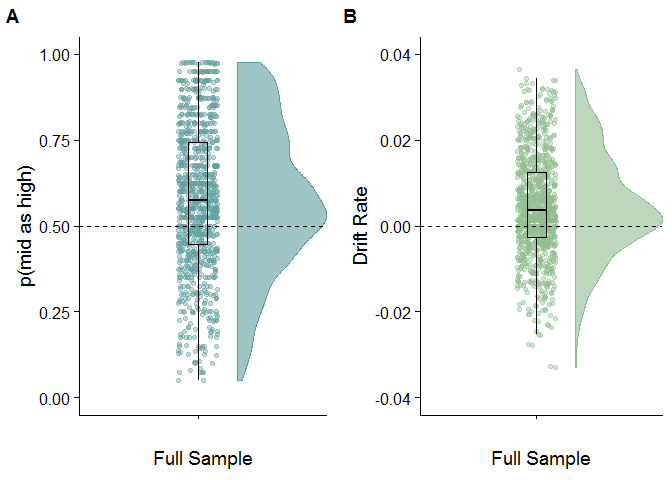
\includegraphics{OpenDataAnalysis_files/figure-latex/unnamed-chunk-4-1.pdf}

\begin{verbatim}
## 
##  One Sample t-test
## 
## data:  combineditemdata$propmedhigh
## t = 12.089, df = 993, p-value < 2.2e-16
## alternative hypothesis: true mean is not equal to 0.5
## 95 percent confidence interval:
##  0.5671525 0.5931778
## sample estimates:
## mean of x 
## 0.5801652
\end{verbatim}

\begin{verbatim}
## 
##  One Sample t-test
## 
## data:  combineditemdata$driftrate
## t = 12.113, df = 993, p-value < 2.2e-16
## alternative hypothesis: true mean is not equal to 0
## 95 percent confidence interval:
##  0.003843921 0.005330160
## sample estimates:
##  mean of x 
## 0.00458704
\end{verbatim}

\begin{longtable}[]{@{}lrrrr@{}}
\toprule
& mean & std & lower range & upper range\tabularnewline
\midrule
\endhead
Age & 34 & 10 & 18 & 76\tabularnewline
Ravens & 4 & 3 & 0 & 12\tabularnewline
OCIR & 42 & 18 & 18 & 90\tabularnewline
SZ & 16 & 9 & 0 & 51\tabularnewline
BDI & 15 & 12 & 0 & 56\tabularnewline
STAI & 45 & 12 & 20 & 78\tabularnewline
\bottomrule
\end{longtable}

\begin{verbatim}
## Split half reliabilities  
## Call: splitHalf(r = dataforsh, raw = T, brute = FALSE, n.sample = 1e+05, 
##     covar = FALSE, check.keys = TRUE, key = NULL, ci = 0.05, 
##     use = "pairwise")
## 
## Maximum split half reliability (lambda 4) =  0.94
## Guttman lambda 6                          =  0.92
## Average split half reliability            =  0.91
## Guttman lambda 3 (alpha)                  =  0.91
## Minimum split half reliability  (beta)    =  0.85
## Average interitem r =  0.21  with median =  0.21
##                                              2.5% 50% 97.5%
##  Quantiles of split half reliability      =  0.9 0.92 0.93
\end{verbatim}

\subsubsection{Simple Linear Regression of
measures}\label{simple-linear-regression-of-measures}

To explore the impact of trait/demographic measures on task performance
we next ran a linear regression (using Robust ML estimator for
consistency with SEM below) to predict p(mid as high)(`propmedhigh'
variable). The variables we included are:

\begin{itemize}
\tightlist
\item
  Spreadsheet (categorical): represents the counterbalancing condition
\item
  Ravens (continuous): IQ measure (visual matrices)
\item
  Age (continuous): years old
\item
  BDI (continuous): Beck depression inventory (suicide question removed)
\item
  STAI2 (continuous): Spielberger Trait Anxiety
\item
  OCIR (continuous): Obsessive-Compulsive Inventory (Revised)
\item
  SZ (continuous): Schizotypal short scale
\item
  GenderMF (categorical): Self-reported gender
\end{itemize}

\begin{Shaded}
\begin{Highlighting}[]
\NormalTok{NegBiasmodel.}\DecValTok{1}\NormalTok{ <-}\StringTok{ 'propmedhigh ~ GenderMF + Age + Ravens + spreadsheet +BDI + STAI2 + SZ + OCIR'}
\NormalTok{NegBiasmodel.}\DecValTok{2}\NormalTok{ <-}\StringTok{ 'driftrate ~ GenderMF + Age + Ravens + spreadsheet +BDI + STAI2 + SZ + OCIR'}


\NormalTok{fit1 <-}\StringTok{ }\KeywordTok{sem}\NormalTok{(NegBiasmodel.}\DecValTok{1}\NormalTok{, }\DataTypeTok{data=}\NormalTok{combineditemdata, }\DataTypeTok{meanstructure=}\OtherTok{TRUE}\NormalTok{,  }\DataTypeTok{estimator =} \StringTok{"MLR"}\NormalTok{)}
\NormalTok{fit2 <-}\StringTok{ }\KeywordTok{sem}\NormalTok{(NegBiasmodel.}\DecValTok{2}\NormalTok{, }\DataTypeTok{data=}\NormalTok{combineditemdata, }\DataTypeTok{meanstructure=}\OtherTok{TRUE}\NormalTok{,  }\DataTypeTok{estimator =} \StringTok{"MLR"}\NormalTok{)}
\NormalTok{fit1miss <-}\StringTok{ }\KeywordTok{sem}\NormalTok{(NegBiasmodel.}\DecValTok{1}\NormalTok{, }\DataTypeTok{data=}\NormalTok{combineditemdata, }\DataTypeTok{meanstructure=}\OtherTok{TRUE}\NormalTok{,  }\DataTypeTok{estimator =} \StringTok{"MLR"}\NormalTok{, }\DataTypeTok{missing =} \StringTok{"ML"}\NormalTok{)}
\NormalTok{fit2miss <-}\StringTok{ }\KeywordTok{sem}\NormalTok{(NegBiasmodel.}\DecValTok{2}\NormalTok{, }\DataTypeTok{data=}\NormalTok{combineditemdata, }\DataTypeTok{meanstructure=}\OtherTok{TRUE}\NormalTok{,  }\DataTypeTok{estimator =} \StringTok{"MLR"}\NormalTok{, }\DataTypeTok{missing =} \StringTok{"ML"}\NormalTok{)}



\KeywordTok{summary}\NormalTok{(fit1, }\DataTypeTok{standardized=}\OtherTok{TRUE}\NormalTok{, }\DataTypeTok{rsquare=}\NormalTok{T, }\DataTypeTok{fit.measures=}\NormalTok{F) }\CommentTok{#listwise delete missing}
\end{Highlighting}
\end{Shaded}

\begin{verbatim}
## lavaan 0.6-3 ended normally after 59 iterations
## 
##   Optimization method                           NLMINB
##   Number of free parameters                         10
## 
##                                                   Used       Total
##   Number of observations                           990        1066
## 
##   Estimator                                         ML      Robust
##   Model Fit Test Statistic                       0.000       0.000
##   Degrees of freedom                                 0           0
##   Minimum Function Value               0.0000000000000
##   Scaling correction factor                                     NA
##     for the Yuan-Bentler correction (Mplus variant)
## 
## Parameter Estimates:
## 
##   Information                                 Observed
##   Observed information based on                Hessian
##   Standard Errors                   Robust.huber.white
## 
## Regressions:
##                    Estimate  Std.Err  z-value  P(>|z|)   Std.lv  Std.all
##   propmedhigh ~                                                         
##     GenderMF         -0.005    0.013   -0.390    0.697   -0.005   -0.012
##     Age              -0.002    0.001   -3.822    0.000   -0.002   -0.120
##     Ravens            0.010    0.002    4.323    0.000    0.010    0.144
##     spreadsheet       0.006    0.002    2.744    0.006    0.006    0.085
##     BDI              -0.002    0.001   -2.373    0.018   -0.002   -0.121
##     STAI2             0.001    0.001    0.789    0.430    0.001    0.037
##     SZ               -0.001    0.001   -1.145    0.252   -0.001   -0.056
##     OCIR              0.000    0.001    0.087    0.931    0.000    0.004
## 
## Intercepts:
##                    Estimate  Std.Err  z-value  P(>|z|)   Std.lv  Std.all
##    .propmedhigh       0.663    0.042   15.791    0.000    0.663    3.166
## 
## Variances:
##                    Estimate  Std.Err  z-value  P(>|z|)   Std.lv  Std.all
##    .propmedhigh       0.041    0.002   24.796    0.000    0.041    0.943
## 
## R-Square:
##                    Estimate
##     propmedhigh       0.057
\end{verbatim}

\begin{Shaded}
\begin{Highlighting}[]
\KeywordTok{summary}\NormalTok{(fit2, }\DataTypeTok{standardized=}\OtherTok{TRUE}\NormalTok{, }\DataTypeTok{rsquare=}\NormalTok{T, }\DataTypeTok{fit.measures=}\NormalTok{F) }\CommentTok{#listwise delete missing}
\end{Highlighting}
\end{Shaded}

\begin{verbatim}
## lavaan 0.6-3 ended normally after 124 iterations
## 
##   Optimization method                           NLMINB
##   Number of free parameters                         10
## 
##                                                   Used       Total
##   Number of observations                           990        1066
## 
##   Estimator                                         ML      Robust
##   Model Fit Test Statistic                       0.000       0.000
##   Degrees of freedom                                 0           0
##   Scaling correction factor                                     NA
##     for the Yuan-Bentler correction (Mplus variant)
## 
## Parameter Estimates:
## 
##   Information                                 Observed
##   Observed information based on                Hessian
##   Standard Errors                   Robust.huber.white
## 
## Regressions:
##                    Estimate  Std.Err  z-value  P(>|z|)   Std.lv  Std.all
##   driftrate ~                                                           
##     GenderMF         -0.000    0.001   -0.421    0.674   -0.000   -0.013
##     Age              -0.000    0.000   -3.611    0.000   -0.000   -0.113
##     Ravens            0.001    0.000    4.348    0.000    0.001    0.146
##     spreadsheet       0.000    0.000    2.766    0.006    0.000    0.086
##     BDI              -0.000    0.000   -2.533    0.011   -0.000   -0.127
##     STAI2             0.000    0.000    0.876    0.381    0.000    0.040
##     SZ               -0.000    0.000   -1.355    0.175   -0.000   -0.066
##     OCIR              0.000    0.000    0.392    0.695    0.000    0.018
## 
## Intercepts:
##                    Estimate  Std.Err  z-value  P(>|z|)   Std.lv  Std.all
##    .driftrate         0.009    0.002    3.707    0.000    0.009    0.740
## 
## Variances:
##                    Estimate  Std.Err  z-value  P(>|z|)   Std.lv  Std.all
##    .driftrate         0.000    0.000   21.371    0.000    0.000    0.943
## 
## R-Square:
##                    Estimate
##     driftrate         0.057
\end{verbatim}

\begin{Shaded}
\begin{Highlighting}[]
\KeywordTok{summary}\NormalTok{(fit1miss, }\DataTypeTok{standardized=}\OtherTok{TRUE}\NormalTok{, }\DataTypeTok{rsquare=}\NormalTok{T, }\DataTypeTok{fit.measures=}\NormalTok{F) }\CommentTok{#estimate missing}
\end{Highlighting}
\end{Shaded}

\begin{verbatim}
## lavaan 0.6-3 ended normally after 59 iterations
## 
##   Optimization method                           NLMINB
##   Number of free parameters                         10
## 
##                                                   Used       Total
##   Number of observations                           990        1066
##   Number of missing patterns                         1
## 
##   Estimator                                         ML      Robust
##   Model Fit Test Statistic                       0.000       0.000
##   Degrees of freedom                                 0           0
##   Scaling correction factor                                     NA
##     for the Yuan-Bentler correction (Mplus variant)
## 
## Parameter Estimates:
## 
##   Information                                 Observed
##   Observed information based on                Hessian
##   Standard Errors                   Robust.huber.white
## 
## Regressions:
##                    Estimate  Std.Err  z-value  P(>|z|)   Std.lv  Std.all
##   propmedhigh ~                                                         
##     GenderMF         -0.005    0.013   -0.390    0.697   -0.005   -0.012
##     Age              -0.002    0.001   -3.822    0.000   -0.002   -0.120
##     Ravens            0.010    0.002    4.323    0.000    0.010    0.144
##     spreadsheet       0.006    0.002    2.744    0.006    0.006    0.085
##     BDI              -0.002    0.001   -2.373    0.018   -0.002   -0.121
##     STAI2             0.001    0.001    0.789    0.430    0.001    0.037
##     SZ               -0.001    0.001   -1.145    0.252   -0.001   -0.056
##     OCIR              0.000    0.001    0.087    0.931    0.000    0.004
## 
## Intercepts:
##                    Estimate  Std.Err  z-value  P(>|z|)   Std.lv  Std.all
##    .propmedhigh       0.663    0.042   15.791    0.000    0.663    3.166
## 
## Variances:
##                    Estimate  Std.Err  z-value  P(>|z|)   Std.lv  Std.all
##    .propmedhigh       0.041    0.002   24.796    0.000    0.041    0.943
## 
## R-Square:
##                    Estimate
##     propmedhigh       0.057
\end{verbatim}

\begin{Shaded}
\begin{Highlighting}[]
\KeywordTok{summary}\NormalTok{(fit2miss, }\DataTypeTok{standardized=}\OtherTok{TRUE}\NormalTok{, }\DataTypeTok{rsquare=}\NormalTok{T, }\DataTypeTok{fit.measures=}\NormalTok{F) }\CommentTok{#estimate missing}
\end{Highlighting}
\end{Shaded}

\begin{verbatim}
## lavaan 0.6-3 ended normally after 120 iterations
## 
##   Optimization method                           NLMINB
##   Number of free parameters                         10
## 
##                                                   Used       Total
##   Number of observations                           990        1066
##   Number of missing patterns                         1
## 
##   Estimator                                         ML      Robust
##   Model Fit Test Statistic                       0.000       0.000
##   Degrees of freedom                                 0           0
##   Scaling correction factor                                     NA
##     for the Yuan-Bentler correction (Mplus variant)
## 
## Parameter Estimates:
## 
##   Information                                 Observed
##   Observed information based on                Hessian
##   Standard Errors                   Robust.huber.white
## 
## Regressions:
##                    Estimate  Std.Err  z-value  P(>|z|)   Std.lv  Std.all
##   driftrate ~                                                           
##     GenderMF         -0.000    0.001   -0.421    0.674   -0.000   -0.013
##     Age              -0.000    0.000   -3.611    0.000   -0.000   -0.113
##     Ravens            0.001    0.000    4.348    0.000    0.001    0.146
##     spreadsheet       0.000    0.000    2.766    0.006    0.000    0.086
##     BDI              -0.000    0.000   -2.533    0.011   -0.000   -0.127
##     STAI2             0.000    0.000    0.876    0.381    0.000    0.040
##     SZ               -0.000    0.000   -1.355    0.175   -0.000   -0.066
##     OCIR              0.000    0.000    0.392    0.695    0.000    0.018
## 
## Intercepts:
##                    Estimate  Std.Err  z-value  P(>|z|)   Std.lv  Std.all
##    .driftrate         0.009    0.002    3.707    0.000    0.009    0.740
## 
## Variances:
##                    Estimate  Std.Err  z-value  P(>|z|)   Std.lv  Std.all
##    .driftrate         0.000    0.000   21.371    0.000    0.000    0.943
## 
## R-Square:
##                    Estimate
##     driftrate         0.057
\end{verbatim}

\paragraph{Interpretation}\label{interpretation-1}

Affective bias and drift rate are both significantly influenced by IQ,
Age, BDI and counterbalancing only. Thus of mental health relevant
symptoms, task performance appears to be more driven by depresson than
anxiety, OCD, or psychosis related traits.

\subsubsection{Correlation between task performance and depression
symptoms}\label{correlation-between-task-performance-and-depression-symptoms}

To illustrate the effect of depression in the regression we plot the
correlation between BDI and pmidhigh/drift rate in raw scores.
Consistent with our prior work, increased depression is associated with
reduced p(mid as high)(i.e.~increased negative bias).

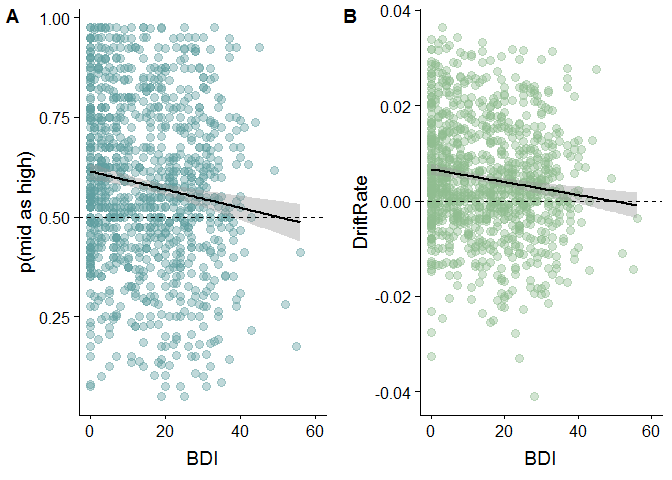
\includegraphics{OpenDataAnalysis_files/figure-latex/unnamed-chunk-6-1.pdf}

\begin{verbatim}
## 
##  Pearson's product-moment correlation
## 
## data:  combineditemdata$BDI and combineditemdata$propmedhigh
## t = -4.1239, df = 992, p-value = 4.036e-05
## alternative hypothesis: true correlation is not equal to 0
## 95 percent confidence interval:
##  -0.19046936 -0.06819752
## sample estimates:
##       cor 
## -0.129827
\end{verbatim}

\begin{verbatim}
## 
##  Pearson's product-moment correlation
## 
## data:  combineditemdata$BDI and combineditemdata$driftrate
## t = -4.2639, df = 992, p-value = 2.2e-05
## alternative hypothesis: true correlation is not equal to 0
## 95 percent confidence interval:
##  -0.19471183 -0.07258157
## sample estimates:
##        cor 
## -0.1341561
\end{verbatim}

\subsubsection{Exploring latent variable structure of the
Questionnaires}\label{exploring-latent-variable-structure-of-the-questionnaires}

The linear regression assumes that the summary scores of the
questionnaires represent discrete categories. However, it is possible
that effects are driven by a generic `mental ill health' factor
(sometimes referred to as a P factor model). Or, some questionnaires
(e.g.~BDI and trait anxiety, which are usually highly correlated)
actually meausure a single latent `negative affect' factor. To test for
these possibilities we explore four confirmatory factor analyses feeding
the individual items from the questionnaires into 1-4 latent factors.
The 4 latent factor CFA represents the items feeding into the original
questionnaires.

\begin{Shaded}
\begin{Highlighting}[]
\NormalTok{###Testing different measurement models}

\NormalTok{pFactor1<-}\StringTok{'#specifying measurement model}

\StringTok{P   =~ BDI_Appetite_quantised   + }
\StringTok{       BDI_Attractive_quantised + }
\StringTok{       BDI_Blame_quantised  + }
\StringTok{       BDI_Cry_quantised    +   }
\StringTok{       BDI_Decisions_quantised  +   }
\StringTok{       BDI_Disappointment_quantised +   }
\StringTok{       BDI_Failure_quantised    +   }
\StringTok{       BDI_Future_quantised +   }
\StringTok{       BDI_Guilty_quantised +   }
\StringTok{       BDI_Health_quantised +   }
\StringTok{       BDI_Interest_In_People_quantised +   }
\StringTok{       BDI_Irritated_quantised  +   }
\StringTok{       BDI_Libido_quantised +   }
\StringTok{       BDI_Punished_quantised   +   }
\StringTok{       BDI_Sad_quantised + }
\StringTok{       BDI_Satisfaction_quantised   +   }
\StringTok{       BDI_Sleep_quantised  +   }
\StringTok{       BDI_Tired_quantised  +   }
\StringTok{       BDI_weight_quantised +   }
\StringTok{       BDI_Work_quantised   +}
\StringTok{        STAI2_Calm_quantised +}
\StringTok{        STAI2_Content_quantised +}
\StringTok{        STAI2_Desicions_quantised +}
\StringTok{        STAI2_Difficulties_quantised +}
\StringTok{        STAI2_DisappointmentsSelf_quantised +}
\StringTok{        STAI2_Failure_quantised +}
\StringTok{        STAI2_Happy_quantised +}
\StringTok{        STAI2_HappyOthers_quantised +}
\StringTok{        STAI2_Inadequate_quantised +}
\StringTok{        STAI2_Nervous_quantised +}
\StringTok{        STAI2_Pleasant_quantised +}
\StringTok{        STAI2_Rested_quantised +}
\StringTok{        STAI2_SatisfiedSelf_quantised +}
\StringTok{        STAI2_Secure_quantised +}
\StringTok{        STAI2_SelfConfidence_quantised +}
\StringTok{        STAI2_Steady_quantised +}
\StringTok{        STAI2_Tension_quantised +}
\StringTok{        STAI2_Thoughts_quantised +}
\StringTok{        STAI2_UnimportantThought_quantised +}
\StringTok{        STAI2_Worry_quantised +}
\StringTok{       OCIR_14_quantised    +   }
\StringTok{       OCIR_15_quantised    +   }
\StringTok{       OCIR_16_quantised    +   }
\StringTok{       OCIR_17_quantised    +   }
\StringTok{       OCIR_18_quantised    +   }
\StringTok{       OCIR_2_quantised +   }
\StringTok{       OCIR_3_quantised +   }
\StringTok{       OCIR_4_quantised +   }
\StringTok{       OCIR_5_quantised +   }
\StringTok{       OCIR_6_quantised +   }
\StringTok{       OCIR_7_quantised +   }
\StringTok{       OCIR_8_quantised +   }
\StringTok{       OCIR_9_quantised +   }
\StringTok{       OCIR_1_quantised +   }
\StringTok{       OCIR_10_quantised    +   }
\StringTok{       OCIR_11_quantised    +   }
\StringTok{       OCIR_12_quantised    +   }
\StringTok{       OCIR_13_quantised  +}
\StringTok{      SZ_1_quantised    +}
\StringTok{      SZ_10_quantised   +   }
\StringTok{      SZ_11_quantised + }
\StringTok{      SZ_12_quantised + }
\StringTok{      SZ_13_quantised + }
\StringTok{      SZ_14_quantised + }
\StringTok{      SZ_15_quantised + }
\StringTok{      SZ_16_quantised + }
\StringTok{      SZ_17_quantised + }
\StringTok{      SZ_18_quantised + }
\StringTok{      SZ_19_quantised + }
\StringTok{      SZ_2_quantised + }
\StringTok{      SZ_20_quantised + }
\StringTok{      SZ_21_quantised + }
\StringTok{      SZ_22_quantised + }
\StringTok{      SZ_23_quantised + }
\StringTok{      SZ_24_quantised + }
\StringTok{      SZ_25_quantised + }
\StringTok{      SZ_26_quantised + }
\StringTok{      SZ_27_quantised + }
\StringTok{      SZ_28_quantised + }
\StringTok{      SZ_29_quantised + }
\StringTok{      SZ_3_quantised + }
\StringTok{      SZ_30_quantised + }
\StringTok{      SZ_31_quantised + }
\StringTok{      SZ_32_quantised + }
\StringTok{      SZ_33_quantised + }
\StringTok{      SZ_34_quantised + }
\StringTok{      SZ_35_quantised + }
\StringTok{      SZ_36_quantised + }
\StringTok{      SZ_37_quantised + }
\StringTok{      SZ_38_quantised + }
\StringTok{      SZ_39_quantised + }
\StringTok{      SZ_4_quantised + }
\StringTok{      SZ_40_quantised + }
\StringTok{      SZ_41_quantised + }
\StringTok{      SZ_42_quantised + }
\StringTok{      SZ_5_quantised + }
\StringTok{      SZ_6_quantised + }
\StringTok{      SZ_7_quantised + }
\StringTok{      SZ_8_quantised + }
\StringTok{      SZ_9_quantised}
\StringTok{'}

\NormalTok{BiFactor2<-}\StringTok{'#specifying measurement model}

\StringTok{ANXDEP =~ BDI_Appetite_quantised    + }
\StringTok{       BDI_Attractive_quantised + }
\StringTok{       BDI_Blame_quantised  + }
\StringTok{       BDI_Cry_quantised    +   }
\StringTok{       BDI_Decisions_quantised  +   }
\StringTok{       BDI_Disappointment_quantised +   }
\StringTok{       BDI_Failure_quantised    +   }
\StringTok{       BDI_Future_quantised +   }
\StringTok{       BDI_Guilty_quantised +   }
\StringTok{       BDI_Health_quantised +   }
\StringTok{       BDI_Interest_In_People_quantised +   }
\StringTok{       BDI_Irritated_quantised  +   }
\StringTok{       BDI_Libido_quantised +   }
\StringTok{       BDI_Punished_quantised   +   }
\StringTok{       BDI_Sad_quantised + }
\StringTok{       BDI_Satisfaction_quantised   +   }
\StringTok{       BDI_Sleep_quantised  +   }
\StringTok{       BDI_Tired_quantised  +   }
\StringTok{       BDI_weight_quantised +   }
\StringTok{       BDI_Work_quantised   +}
\StringTok{        STAI2_Calm_quantised +}
\StringTok{        STAI2_Content_quantised +}
\StringTok{        STAI2_Desicions_quantised +}
\StringTok{        STAI2_Difficulties_quantised +}
\StringTok{        STAI2_DisappointmentsSelf_quantised +}
\StringTok{        STAI2_Failure_quantised +}
\StringTok{        STAI2_Happy_quantised +}
\StringTok{        STAI2_HappyOthers_quantised +}
\StringTok{        STAI2_Inadequate_quantised +}
\StringTok{        STAI2_Nervous_quantised +}
\StringTok{        STAI2_Pleasant_quantised +}
\StringTok{        STAI2_Rested_quantised +}
\StringTok{        STAI2_SatisfiedSelf_quantised +}
\StringTok{        STAI2_Secure_quantised +}
\StringTok{        STAI2_SelfConfidence_quantised +}
\StringTok{        STAI2_Steady_quantised +}
\StringTok{        STAI2_Tension_quantised +}
\StringTok{        STAI2_Thoughts_quantised +}
\StringTok{        STAI2_UnimportantThought_quantised +}
\StringTok{        STAI2_Worry_quantised}

\StringTok{OTH =~ OCIR_14_quantised    +   }
\StringTok{       OCIR_15_quantised    +   }
\StringTok{       OCIR_16_quantised    +   }
\StringTok{       OCIR_17_quantised    +   }
\StringTok{       OCIR_18_quantised    +   }
\StringTok{       OCIR_2_quantised +   }
\StringTok{       OCIR_3_quantised +   }
\StringTok{       OCIR_4_quantised +   }
\StringTok{       OCIR_5_quantised +   }
\StringTok{       OCIR_6_quantised +   }
\StringTok{       OCIR_7_quantised +   }
\StringTok{       OCIR_8_quantised +   }
\StringTok{       OCIR_9_quantised +   }
\StringTok{       OCIR_1_quantised +   }
\StringTok{       OCIR_10_quantised    +   }
\StringTok{       OCIR_11_quantised    +   }
\StringTok{       OCIR_12_quantised    +   }
\StringTok{       OCIR_13_quantised  +}
\StringTok{      SZ_1_quantised    +}
\StringTok{      SZ_10_quantised   +   }
\StringTok{      SZ_11_quantised + }
\StringTok{      SZ_12_quantised + }
\StringTok{      SZ_13_quantised + }
\StringTok{      SZ_14_quantised + }
\StringTok{      SZ_15_quantised + }
\StringTok{      SZ_16_quantised + }
\StringTok{      SZ_17_quantised + }
\StringTok{      SZ_18_quantised + }
\StringTok{      SZ_19_quantised + }
\StringTok{      SZ_2_quantised + }
\StringTok{      SZ_20_quantised + }
\StringTok{      SZ_21_quantised + }
\StringTok{      SZ_22_quantised + }
\StringTok{      SZ_23_quantised + }
\StringTok{      SZ_24_quantised + }
\StringTok{      SZ_25_quantised + }
\StringTok{      SZ_26_quantised + }
\StringTok{      SZ_27_quantised + }
\StringTok{      SZ_28_quantised + }
\StringTok{      SZ_29_quantised + }
\StringTok{      SZ_3_quantised + }
\StringTok{      SZ_30_quantised + }
\StringTok{      SZ_31_quantised + }
\StringTok{      SZ_32_quantised + }
\StringTok{      SZ_33_quantised + }
\StringTok{      SZ_34_quantised + }
\StringTok{      SZ_35_quantised + }
\StringTok{      SZ_36_quantised + }
\StringTok{      SZ_37_quantised + }
\StringTok{      SZ_38_quantised + }
\StringTok{      SZ_39_quantised + }
\StringTok{      SZ_4_quantised + }
\StringTok{      SZ_40_quantised + }
\StringTok{      SZ_41_quantised + }
\StringTok{      SZ_42_quantised + }
\StringTok{      SZ_5_quantised + }
\StringTok{      SZ_6_quantised + }
\StringTok{      SZ_7_quantised + }
\StringTok{      SZ_8_quantised + }
\StringTok{      SZ_9_quantised}
\StringTok{'}

\NormalTok{TriFactor3<-}\StringTok{'#specifying measurement model}

\StringTok{ANXDEP =~ BDI_Appetite_quantised    + }
\StringTok{       BDI_Attractive_quantised + }
\StringTok{       BDI_Blame_quantised  + }
\StringTok{       BDI_Cry_quantised    +   }
\StringTok{       BDI_Decisions_quantised  +   }
\StringTok{       BDI_Disappointment_quantised +   }
\StringTok{       BDI_Failure_quantised    +   }
\StringTok{       BDI_Future_quantised +   }
\StringTok{       BDI_Guilty_quantised +   }
\StringTok{       BDI_Health_quantised +   }
\StringTok{       BDI_Interest_In_People_quantised +   }
\StringTok{       BDI_Irritated_quantised  +   }
\StringTok{       BDI_Libido_quantised +   }
\StringTok{       BDI_Punished_quantised   +   }
\StringTok{       BDI_Sad_quantised + }
\StringTok{       BDI_Satisfaction_quantised   +   }
\StringTok{       BDI_Sleep_quantised  +   }
\StringTok{       BDI_Tired_quantised  +   }
\StringTok{       BDI_weight_quantised +   }
\StringTok{       BDI_Work_quantised   +}
\StringTok{        STAI2_Calm_quantised +}
\StringTok{        STAI2_Content_quantised +}
\StringTok{        STAI2_Desicions_quantised +}
\StringTok{        STAI2_Difficulties_quantised +}
\StringTok{        STAI2_DisappointmentsSelf_quantised +}
\StringTok{        STAI2_Failure_quantised +}
\StringTok{        STAI2_Happy_quantised +}
\StringTok{        STAI2_HappyOthers_quantised +}
\StringTok{        STAI2_Inadequate_quantised +}
\StringTok{        STAI2_Nervous_quantised +}
\StringTok{        STAI2_Pleasant_quantised +}
\StringTok{        STAI2_Rested_quantised +}
\StringTok{        STAI2_SatisfiedSelf_quantised +}
\StringTok{        STAI2_Secure_quantised +}
\StringTok{        STAI2_SelfConfidence_quantised +}
\StringTok{        STAI2_Steady_quantised +}
\StringTok{        STAI2_Tension_quantised +}
\StringTok{        STAI2_Thoughts_quantised +}
\StringTok{        STAI2_UnimportantThought_quantised +}
\StringTok{        STAI2_Worry_quantised}

\StringTok{OCD =~ OCIR_14_quantised    +   }
\StringTok{       OCIR_15_quantised    +   }
\StringTok{       OCIR_16_quantised    +   }
\StringTok{       OCIR_17_quantised    +   }
\StringTok{       OCIR_18_quantised    +   }
\StringTok{       OCIR_2_quantised +   }
\StringTok{       OCIR_3_quantised +   }
\StringTok{       OCIR_4_quantised +   }
\StringTok{       OCIR_5_quantised +   }
\StringTok{       OCIR_6_quantised +   }
\StringTok{       OCIR_7_quantised +   }
\StringTok{       OCIR_8_quantised +   }
\StringTok{       OCIR_9_quantised +   }
\StringTok{       OCIR_1_quantised +   }
\StringTok{       OCIR_10_quantised    +   }
\StringTok{       OCIR_11_quantised    +   }
\StringTok{       OCIR_12_quantised    +   }
\StringTok{       OCIR_13_quantised}

\StringTok{SZ =~ SZ_1_quantised    +}
\StringTok{      SZ_10_quantised   +   }
\StringTok{      SZ_11_quantised + }
\StringTok{      SZ_12_quantised + }
\StringTok{      SZ_13_quantised + }
\StringTok{      SZ_14_quantised + }
\StringTok{      SZ_15_quantised + }
\StringTok{      SZ_16_quantised + }
\StringTok{      SZ_17_quantised + }
\StringTok{      SZ_18_quantised + }
\StringTok{      SZ_19_quantised + }
\StringTok{      SZ_2_quantised + }
\StringTok{      SZ_20_quantised + }
\StringTok{      SZ_21_quantised + }
\StringTok{      SZ_22_quantised + }
\StringTok{      SZ_23_quantised + }
\StringTok{      SZ_24_quantised + }
\StringTok{      SZ_25_quantised + }
\StringTok{      SZ_26_quantised + }
\StringTok{      SZ_27_quantised + }
\StringTok{      SZ_28_quantised + }
\StringTok{      SZ_29_quantised + }
\StringTok{      SZ_3_quantised + }
\StringTok{      SZ_30_quantised + }
\StringTok{      SZ_31_quantised + }
\StringTok{      SZ_32_quantised + }
\StringTok{      SZ_33_quantised + }
\StringTok{      SZ_34_quantised + }
\StringTok{      SZ_35_quantised + }
\StringTok{      SZ_36_quantised + }
\StringTok{      SZ_37_quantised + }
\StringTok{      SZ_38_quantised + }
\StringTok{      SZ_39_quantised + }
\StringTok{      SZ_4_quantised + }
\StringTok{      SZ_40_quantised + }
\StringTok{      SZ_41_quantised + }
\StringTok{      SZ_42_quantised + }
\StringTok{      SZ_5_quantised + }
\StringTok{      SZ_6_quantised + }
\StringTok{      SZ_7_quantised + }
\StringTok{      SZ_8_quantised + }
\StringTok{      SZ_9_quantised}
\StringTok{'}
\NormalTok{Quaires4 <-}\StringTok{'#specifying measurement model}

\StringTok{BDI =~ BDI_Appetite_quantised   + }
\StringTok{       BDI_Attractive_quantised + }
\StringTok{       BDI_Blame_quantised  + }
\StringTok{       BDI_Cry_quantised    +   }
\StringTok{       BDI_Decisions_quantised  +   }
\StringTok{       BDI_Disappointment_quantised +   }
\StringTok{       BDI_Failure_quantised    +   }
\StringTok{       BDI_Future_quantised +   }
\StringTok{       BDI_Guilty_quantised +   }
\StringTok{       BDI_Health_quantised +   }
\StringTok{       BDI_Interest_In_People_quantised +   }
\StringTok{       BDI_Irritated_quantised  +   }
\StringTok{       BDI_Libido_quantised +   }
\StringTok{       BDI_Punished_quantised   +   }
\StringTok{       BDI_Sad_quantised + }
\StringTok{       BDI_Satisfaction_quantised   +   }
\StringTok{       BDI_Sleep_quantised  +   }
\StringTok{       BDI_Tired_quantised  +   }
\StringTok{       BDI_weight_quantised +   }
\StringTok{       BDI_Work_quantised   }

\StringTok{OCD =~ OCIR_14_quantised    +   }
\StringTok{       OCIR_15_quantised    +   }
\StringTok{       OCIR_16_quantised    +   }
\StringTok{       OCIR_17_quantised    +   }
\StringTok{       OCIR_18_quantised    +   }
\StringTok{       OCIR_2_quantised +   }
\StringTok{       OCIR_3_quantised +   }
\StringTok{       OCIR_4_quantised +   }
\StringTok{       OCIR_5_quantised +   }
\StringTok{       OCIR_6_quantised +   }
\StringTok{       OCIR_7_quantised +   }
\StringTok{       OCIR_8_quantised +   }
\StringTok{       OCIR_9_quantised +   }
\StringTok{       OCIR_1_quantised +   }
\StringTok{       OCIR_10_quantised    +   }
\StringTok{       OCIR_11_quantised    +   }
\StringTok{       OCIR_12_quantised    +   }
\StringTok{       OCIR_13_quantised}

\StringTok{SZ =~ SZ_1_quantised    +}
\StringTok{      SZ_10_quantised   +   }
\StringTok{      SZ_11_quantised + }
\StringTok{      SZ_12_quantised + }
\StringTok{      SZ_13_quantised + }
\StringTok{      SZ_14_quantised + }
\StringTok{      SZ_15_quantised + }
\StringTok{      SZ_16_quantised + }
\StringTok{      SZ_17_quantised + }
\StringTok{      SZ_18_quantised + }
\StringTok{      SZ_19_quantised + }
\StringTok{      SZ_2_quantised + }
\StringTok{      SZ_20_quantised + }
\StringTok{      SZ_21_quantised + }
\StringTok{      SZ_22_quantised + }
\StringTok{      SZ_23_quantised + }
\StringTok{      SZ_24_quantised + }
\StringTok{      SZ_25_quantised + }
\StringTok{      SZ_26_quantised + }
\StringTok{      SZ_27_quantised + }
\StringTok{      SZ_28_quantised + }
\StringTok{      SZ_29_quantised + }
\StringTok{      SZ_3_quantised + }
\StringTok{      SZ_30_quantised + }
\StringTok{      SZ_31_quantised + }
\StringTok{      SZ_32_quantised + }
\StringTok{      SZ_33_quantised + }
\StringTok{      SZ_34_quantised + }
\StringTok{      SZ_35_quantised + }
\StringTok{      SZ_36_quantised + }
\StringTok{      SZ_37_quantised + }
\StringTok{      SZ_38_quantised + }
\StringTok{      SZ_39_quantised + }
\StringTok{      SZ_4_quantised + }
\StringTok{      SZ_40_quantised + }
\StringTok{      SZ_41_quantised + }
\StringTok{      SZ_42_quantised + }
\StringTok{      SZ_5_quantised + }
\StringTok{      SZ_6_quantised + }
\StringTok{      SZ_7_quantised + }
\StringTok{      SZ_8_quantised + }
\StringTok{      SZ_9_quantised}

\StringTok{STAI =~ STAI2_Calm_quantised +}
\StringTok{        STAI2_Content_quantised +}
\StringTok{        STAI2_Desicions_quantised +}
\StringTok{        STAI2_Difficulties_quantised +}
\StringTok{        STAI2_DisappointmentsSelf_quantised +}
\StringTok{        STAI2_Failure_quantised +}
\StringTok{        STAI2_Happy_quantised +}
\StringTok{        STAI2_HappyOthers_quantised +}
\StringTok{        STAI2_Inadequate_quantised +}
\StringTok{        STAI2_Nervous_quantised +}
\StringTok{        STAI2_Pleasant_quantised +}
\StringTok{        STAI2_Rested_quantised +}
\StringTok{        STAI2_SatisfiedSelf_quantised +}
\StringTok{        STAI2_Secure_quantised +}
\StringTok{        STAI2_SelfConfidence_quantised +}
\StringTok{        STAI2_Steady_quantised +}
\StringTok{        STAI2_Tension_quantised +}
\StringTok{        STAI2_Thoughts_quantised +}
\StringTok{        STAI2_UnimportantThought_quantised +}
\StringTok{        STAI2_Worry_quantised}
\StringTok{'}

\NormalTok{FitpFactor1<-}\StringTok{ }\KeywordTok{cfa}\NormalTok{(pFactor1, }\DataTypeTok{data =}\NormalTok{ combineditemdata, }\DataTypeTok{estimator =} \StringTok{"MLR"}\NormalTok{, }\DataTypeTok{se=}\StringTok{'robust.huber.white'}\NormalTok{)}
\NormalTok{FitBiFactor2<-}\StringTok{ }\KeywordTok{cfa}\NormalTok{(BiFactor2, }\DataTypeTok{data =}\NormalTok{ combineditemdata, }\DataTypeTok{estimator =} \StringTok{"MLR"}\NormalTok{, }\DataTypeTok{se=}\StringTok{'robust.huber.white'}\NormalTok{)}
\NormalTok{FitTriFactor3<-}\StringTok{ }\KeywordTok{cfa}\NormalTok{(TriFactor3, }\DataTypeTok{data =}\NormalTok{ combineditemdata, }\DataTypeTok{estimator =} \StringTok{"MLR"}\NormalTok{, }\DataTypeTok{se=}\StringTok{'robust.huber.white'}\NormalTok{)}
\NormalTok{FitQuaires4<-}\StringTok{ }\KeywordTok{cfa}\NormalTok{(Quaires4, }\DataTypeTok{data =}\NormalTok{ combineditemdata, }\DataTypeTok{estimator =} \StringTok{"MLR"}\NormalTok{, }\DataTypeTok{se=}\StringTok{'robust.huber.white'}\NormalTok{)}

\NormalTok{FitpFactor1vars <-}\KeywordTok{data.frame}\NormalTok{(}\KeywordTok{fitMeasures}\NormalTok{(FitpFactor1, }\KeywordTok{c}\NormalTok{(}\StringTok{"bic"}\NormalTok{,}\StringTok{"aic"}\NormalTok{,}\StringTok{"rmsea"}\NormalTok{,}\StringTok{"rmsea.ci.lower"}\NormalTok{, }\StringTok{"rmsea.ci.upper"}\NormalTok{)))}
\KeywordTok{names}\NormalTok{(FitpFactor1vars) <-}\StringTok{ "P Factor"}
\NormalTok{FitBiFactor2vars<-}\StringTok{ }\KeywordTok{data.frame}\NormalTok{(}\KeywordTok{fitMeasures}\NormalTok{(FitBiFactor2, }\KeywordTok{c}\NormalTok{(}\StringTok{"bic"}\NormalTok{,}\StringTok{"aic"}\NormalTok{,}\StringTok{"rmsea"}\NormalTok{,}\StringTok{"rmsea.ci.lower"}\NormalTok{, }\StringTok{"rmsea.ci.upper"}\NormalTok{)))}
\KeywordTok{names}\NormalTok{(FitBiFactor2vars) <-}\StringTok{ "Bi Factor (AnxDep vs. not)"}
\NormalTok{FitTriFactor3vars<-}\StringTok{ }\KeywordTok{data.frame}\NormalTok{(}\KeywordTok{fitMeasures}\NormalTok{(FitTriFactor3, }\KeywordTok{c}\NormalTok{(}\StringTok{"bic"}\NormalTok{,}\StringTok{"aic"}\NormalTok{,}\StringTok{"rmsea"}\NormalTok{,}\StringTok{"rmsea.ci.lower"}\NormalTok{, }\StringTok{"rmsea.ci.upper"}\NormalTok{)))}
\KeywordTok{names}\NormalTok{(FitTriFactor3vars) <-}\StringTok{ "Tri Factor (AnxDep vs. SZ or OCD)"}
\NormalTok{FitQuaires4vars<-}\StringTok{ }\KeywordTok{data.frame}\NormalTok{(}\KeywordTok{fitMeasures}\NormalTok{(FitQuaires4, }\KeywordTok{c}\NormalTok{(}\StringTok{"bic"}\NormalTok{,}\StringTok{"aic"}\NormalTok{,}\StringTok{"rmsea"}\NormalTok{,}\StringTok{"rmsea.ci.lower"}\NormalTok{, }\StringTok{"rmsea.ci.upper"}\NormalTok{)))}
\KeywordTok{names}\NormalTok{(FitQuaires4vars) <-}\StringTok{ "Four Factor (All questionnaires)"}
\NormalTok{Allfits <-}\StringTok{ }\KeywordTok{cbind.data.frame}\NormalTok{(FitpFactor1vars, FitBiFactor2vars, FitTriFactor3vars, FitQuaires4vars)}
\KeywordTok{rownames}\NormalTok{(Allfits) <-}\StringTok{ }\KeywordTok{c}\NormalTok{(}\StringTok{"BIC"}\NormalTok{, }\StringTok{"AIC"}\NormalTok{, }\StringTok{"RMSEA"}\NormalTok{, }\StringTok{"RMSEA CI-"}\NormalTok{, }\StringTok{"RMSEA CI+"}\NormalTok{)}

\KeywordTok{kable}\NormalTok{(}\KeywordTok{t}\NormalTok{(Allfits), }\DataTypeTok{digits =} \DecValTok{3}\NormalTok{)}
\end{Highlighting}
\end{Shaded}

\begin{longtable}[]{@{}lrrrrr@{}}
\toprule
& BIC & AIC & RMSEA & RMSEA CI- & RMSEA CI+\tabularnewline
\midrule
\endhead
P Factor & 206756.6 & 205762.2 & 0.071 & 0.071 & 0.072\tabularnewline
Bi Factor (AnxDep vs.~not) & 199828.5 & 198829.1 & 0.061 & 0.060 &
0.062\tabularnewline
Tri Factor (AnxDep vs.~SZ or OCD) & 196936.3 & 195927.1 & 0.056 & 0.056
& 0.057\tabularnewline
Four Factor (All questionnaires) & 195624.0 & 194599.8 & 0.054 & 0.053 &
0.055\tabularnewline
\bottomrule
\end{longtable}

\paragraph{Interpretation}\label{interpretation-2}

As demonstrated by the lowest BIC/AIC the 4 factor (orignal
questionnaire structure) solution is the best description of the data.
This also has the lowest RMSEA, which is in turn below 0.08 and hence a
good fit to the data.

\subsubsection{Structural Equation Model of the factor structure with
regression}\label{structural-equation-model-of-the-factor-structure-with-regression}

We can now feed this factor structure into a structural equation model
with the original regression analysis in it. This is similar to the
linear regression, although it allows the different items of the
questionnaire to have varying influence over the summary questionnaire
`factors'.

\begin{Shaded}
\begin{Highlighting}[]
\NormalTok{###SEM}

\NormalTok{QuaireSEMpmid <-}\StringTok{ '#specifying measurement model}

\StringTok{BDI =~ BDI_Appetite_quantised   + }
\StringTok{       BDI_Attractive_quantised + }
\StringTok{       BDI_Blame_quantised  + }
\StringTok{       BDI_Cry_quantised    +   }
\StringTok{       BDI_Decisions_quantised  +   }
\StringTok{       BDI_Disappointment_quantised +   }
\StringTok{       BDI_Failure_quantised    +   }
\StringTok{       BDI_Future_quantised +   }
\StringTok{       BDI_Guilty_quantised +   }
\StringTok{       BDI_Health_quantised +   }
\StringTok{       BDI_Interest_In_People_quantised +   }
\StringTok{       BDI_Irritated_quantised  +   }
\StringTok{       BDI_Libido_quantised +   }
\StringTok{       BDI_Punished_quantised   +   }
\StringTok{       BDI_Sad_quantised + }
\StringTok{       BDI_Satisfaction_quantised   +   }
\StringTok{       BDI_Sleep_quantised  +   }
\StringTok{       BDI_Tired_quantised  +   }
\StringTok{       BDI_weight_quantised +   }
\StringTok{       BDI_Work_quantised   }

\StringTok{OCD =~ OCIR_14_quantised    +   }
\StringTok{       OCIR_15_quantised    +   }
\StringTok{       OCIR_16_quantised    +   }
\StringTok{       OCIR_17_quantised    +   }
\StringTok{       OCIR_18_quantised    +   }
\StringTok{       OCIR_2_quantised +   }
\StringTok{       OCIR_3_quantised +   }
\StringTok{       OCIR_4_quantised +   }
\StringTok{       OCIR_5_quantised +   }
\StringTok{       OCIR_6_quantised +   }
\StringTok{       OCIR_7_quantised +   }
\StringTok{       OCIR_8_quantised +   }
\StringTok{       OCIR_9_quantised +   }
\StringTok{       OCIR_1_quantised +   }
\StringTok{       OCIR_10_quantised    +   }
\StringTok{       OCIR_11_quantised    +   }
\StringTok{       OCIR_12_quantised    +   }
\StringTok{       OCIR_13_quantised}

\StringTok{SZ =~ SZ_1_quantised    +}
\StringTok{      SZ_10_quantised   +   }
\StringTok{      SZ_11_quantised + }
\StringTok{      SZ_12_quantised + }
\StringTok{      SZ_13_quantised + }
\StringTok{      SZ_14_quantised + }
\StringTok{      SZ_15_quantised + }
\StringTok{      SZ_16_quantised + }
\StringTok{      SZ_17_quantised + }
\StringTok{      SZ_18_quantised + }
\StringTok{      SZ_19_quantised + }
\StringTok{      SZ_2_quantised + }
\StringTok{      SZ_20_quantised + }
\StringTok{      SZ_21_quantised + }
\StringTok{      SZ_22_quantised + }
\StringTok{      SZ_23_quantised + }
\StringTok{      SZ_24_quantised + }
\StringTok{      SZ_25_quantised + }
\StringTok{      SZ_26_quantised + }
\StringTok{      SZ_27_quantised + }
\StringTok{      SZ_28_quantised + }
\StringTok{      SZ_29_quantised + }
\StringTok{      SZ_3_quantised + }
\StringTok{      SZ_30_quantised + }
\StringTok{      SZ_31_quantised + }
\StringTok{      SZ_32_quantised + }
\StringTok{      SZ_33_quantised + }
\StringTok{      SZ_34_quantised + }
\StringTok{      SZ_35_quantised + }
\StringTok{      SZ_36_quantised + }
\StringTok{      SZ_37_quantised + }
\StringTok{      SZ_38_quantised + }
\StringTok{      SZ_39_quantised + }
\StringTok{      SZ_4_quantised + }
\StringTok{      SZ_40_quantised + }
\StringTok{      SZ_41_quantised + }
\StringTok{      SZ_42_quantised + }
\StringTok{      SZ_5_quantised + }
\StringTok{      SZ_6_quantised + }
\StringTok{      SZ_7_quantised + }
\StringTok{      SZ_8_quantised + }
\StringTok{      SZ_9_quantised}

\StringTok{STAI =~ STAI2_Calm_quantised +}
\StringTok{        STAI2_Content_quantised +}
\StringTok{        STAI2_Desicions_quantised +}
\StringTok{        STAI2_Difficulties_quantised +}
\StringTok{        STAI2_DisappointmentsSelf_quantised +}
\StringTok{        STAI2_Failure_quantised +}
\StringTok{        STAI2_Happy_quantised +}
\StringTok{        STAI2_HappyOthers_quantised +}
\StringTok{        STAI2_Inadequate_quantised +}
\StringTok{        STAI2_Nervous_quantised +}
\StringTok{        STAI2_Pleasant_quantised +}
\StringTok{        STAI2_Rested_quantised +}
\StringTok{        STAI2_SatisfiedSelf_quantised +}
\StringTok{        STAI2_Secure_quantised +}
\StringTok{        STAI2_SelfConfidence_quantised +}
\StringTok{        STAI2_Steady_quantised +}
\StringTok{        STAI2_Tension_quantised +}
\StringTok{        STAI2_Thoughts_quantised +}
\StringTok{        STAI2_UnimportantThought_quantised +}
\StringTok{        STAI2_Worry_quantised}


\StringTok{#Regressions}
\StringTok{propmedhigh ~ spreadsheet + Ravens + Age + GenderMF + BDI + OCD + SZ + STAI}

\StringTok{#residual correlations}
\StringTok{spreadsheet ~~ Ravens + Age + GenderMF + BDI + OCD + SZ + STAI}
\StringTok{Ravens ~~ Age  + GenderMF + BDI + OCD + SZ + STAI}
\StringTok{Age ~~  GenderMF + BDI + OCD + SZ + STAI}
\StringTok{GenderMF ~~ BDI + OCD + SZ + STAI}
\StringTok{BDI ~~ OCD + SZ + STAI}
\StringTok{OCD ~~ SZ + STAI}
\StringTok{SZ ~~ STAI}
\StringTok{'}

\NormalTok{QuaireSEMdrift <-}\StringTok{ '#specifying measurement model}

\StringTok{BDI =~ BDI_Appetite_quantised   + }
\StringTok{       BDI_Attractive_quantised + }
\StringTok{       BDI_Blame_quantised  + }
\StringTok{       BDI_Cry_quantised    +   }
\StringTok{       BDI_Decisions_quantised  +   }
\StringTok{       BDI_Disappointment_quantised +   }
\StringTok{       BDI_Failure_quantised    +   }
\StringTok{       BDI_Future_quantised +   }
\StringTok{       BDI_Guilty_quantised +   }
\StringTok{       BDI_Health_quantised +   }
\StringTok{       BDI_Interest_In_People_quantised +   }
\StringTok{       BDI_Irritated_quantised  +   }
\StringTok{       BDI_Libido_quantised +   }
\StringTok{       BDI_Punished_quantised   +   }
\StringTok{       BDI_Sad_quantised + }
\StringTok{       BDI_Satisfaction_quantised   +   }
\StringTok{       BDI_Sleep_quantised  +   }
\StringTok{       BDI_Tired_quantised  +   }
\StringTok{       BDI_weight_quantised +   }
\StringTok{       BDI_Work_quantised   }

\StringTok{OCD =~ OCIR_14_quantised    +   }
\StringTok{       OCIR_15_quantised    +   }
\StringTok{       OCIR_16_quantised    +   }
\StringTok{       OCIR_17_quantised    +   }
\StringTok{       OCIR_18_quantised    +   }
\StringTok{       OCIR_2_quantised +   }
\StringTok{       OCIR_3_quantised +   }
\StringTok{       OCIR_4_quantised +   }
\StringTok{       OCIR_5_quantised +   }
\StringTok{       OCIR_6_quantised +   }
\StringTok{       OCIR_7_quantised +   }
\StringTok{       OCIR_8_quantised +   }
\StringTok{       OCIR_9_quantised +   }
\StringTok{       OCIR_1_quantised +   }
\StringTok{       OCIR_10_quantised    +   }
\StringTok{       OCIR_11_quantised    +   }
\StringTok{       OCIR_12_quantised    +   }
\StringTok{       OCIR_13_quantised}

\StringTok{SZ =~ SZ_1_quantised    +}
\StringTok{      SZ_10_quantised   +   }
\StringTok{      SZ_11_quantised + }
\StringTok{      SZ_12_quantised + }
\StringTok{      SZ_13_quantised + }
\StringTok{      SZ_14_quantised + }
\StringTok{      SZ_15_quantised + }
\StringTok{      SZ_16_quantised + }
\StringTok{      SZ_17_quantised + }
\StringTok{      SZ_18_quantised + }
\StringTok{      SZ_19_quantised + }
\StringTok{      SZ_2_quantised + }
\StringTok{      SZ_20_quantised + }
\StringTok{      SZ_21_quantised + }
\StringTok{      SZ_22_quantised + }
\StringTok{      SZ_23_quantised + }
\StringTok{      SZ_24_quantised + }
\StringTok{      SZ_25_quantised + }
\StringTok{      SZ_26_quantised + }
\StringTok{      SZ_27_quantised + }
\StringTok{      SZ_28_quantised + }
\StringTok{      SZ_29_quantised + }
\StringTok{      SZ_3_quantised + }
\StringTok{      SZ_30_quantised + }
\StringTok{      SZ_31_quantised + }
\StringTok{      SZ_32_quantised + }
\StringTok{      SZ_33_quantised + }
\StringTok{      SZ_34_quantised + }
\StringTok{      SZ_35_quantised + }
\StringTok{      SZ_36_quantised + }
\StringTok{      SZ_37_quantised + }
\StringTok{      SZ_38_quantised + }
\StringTok{      SZ_39_quantised + }
\StringTok{      SZ_4_quantised + }
\StringTok{      SZ_40_quantised + }
\StringTok{      SZ_41_quantised + }
\StringTok{      SZ_42_quantised + }
\StringTok{      SZ_5_quantised + }
\StringTok{      SZ_6_quantised + }
\StringTok{      SZ_7_quantised + }
\StringTok{      SZ_8_quantised + }
\StringTok{      SZ_9_quantised}

\StringTok{STAI =~ STAI2_Calm_quantised +}
\StringTok{        STAI2_Content_quantised +}
\StringTok{        STAI2_Desicions_quantised +}
\StringTok{        STAI2_Difficulties_quantised +}
\StringTok{        STAI2_DisappointmentsSelf_quantised +}
\StringTok{        STAI2_Failure_quantised +}
\StringTok{        STAI2_Happy_quantised +}
\StringTok{        STAI2_HappyOthers_quantised +}
\StringTok{        STAI2_Inadequate_quantised +}
\StringTok{        STAI2_Nervous_quantised +}
\StringTok{        STAI2_Pleasant_quantised +}
\StringTok{        STAI2_Rested_quantised +}
\StringTok{        STAI2_SatisfiedSelf_quantised +}
\StringTok{        STAI2_Secure_quantised +}
\StringTok{        STAI2_SelfConfidence_quantised +}
\StringTok{        STAI2_Steady_quantised +}
\StringTok{        STAI2_Tension_quantised +}
\StringTok{        STAI2_Thoughts_quantised +}
\StringTok{        STAI2_UnimportantThought_quantised +}
\StringTok{        STAI2_Worry_quantised}


\StringTok{#Regressions}
\StringTok{driftrate ~ spreadsheet + Ravens + Age + GenderMF + BDI + OCD + SZ + STAI}

\StringTok{#residual correlations}
\StringTok{spreadsheet ~~ Ravens + Age + GenderMF + BDI + OCD + SZ + STAI}
\StringTok{Ravens ~~ Age  + GenderMF + BDI + OCD + SZ + STAI}
\StringTok{Age ~~  GenderMF + BDI + OCD + SZ + STAI}
\StringTok{GenderMF ~~ BDI + OCD + SZ + STAI}
\StringTok{BDI ~~ OCD + SZ + STAI}
\StringTok{OCD ~~ SZ + STAI}
\StringTok{SZ ~~ STAI}
\StringTok{'}

\NormalTok{FitQuaireSEMpmid <-}\StringTok{ }\KeywordTok{sem}\NormalTok{(QuaireSEMpmid, }\DataTypeTok{data =}\NormalTok{ combineditemdata, }\DataTypeTok{estimator =} \StringTok{"MLR"}\NormalTok{, }\DataTypeTok{se=}\StringTok{'robust.huber.white'}\NormalTok{)}
\NormalTok{FitQuaireSEMdrift <-}\StringTok{ }\KeywordTok{sem}\NormalTok{(QuaireSEMdrift, }\DataTypeTok{data =}\NormalTok{ combineditemdata, }\DataTypeTok{estimator =} \StringTok{"MLR"}\NormalTok{, }\DataTypeTok{se=}\StringTok{'robust.huber.white'}\NormalTok{)}

\NormalTok{FitQuaireSEMpmidmiss <-}\StringTok{ }\KeywordTok{sem}\NormalTok{(QuaireSEMpmid, }\DataTypeTok{data =}\NormalTok{ combineditemdata, }\DataTypeTok{estimator =} \StringTok{"MLR"}\NormalTok{, }\DataTypeTok{se=}\StringTok{'robust.huber.white'}\NormalTok{, }\DataTypeTok{missing =} \StringTok{"ML"}\NormalTok{)}
\NormalTok{FitQuaireSEMdriftmiss <-}\StringTok{ }\KeywordTok{sem}\NormalTok{(QuaireSEMdrift, }\DataTypeTok{data =}\NormalTok{ combineditemdata, }\DataTypeTok{estimator =} \StringTok{"MLR"}\NormalTok{, }\DataTypeTok{se=}\StringTok{'robust.huber.white'}\NormalTok{, }\DataTypeTok{missing =} \StringTok{"ML"}\NormalTok{)}

\KeywordTok{summary}\NormalTok{(FitQuaireSEMpmid, }\DataTypeTok{standardized=}\OtherTok{TRUE}\NormalTok{, }\DataTypeTok{rsquare=}\NormalTok{T, }\DataTypeTok{fit.measures=}\NormalTok{F) }\CommentTok{#listwise delete missing}
\end{Highlighting}
\end{Shaded}

\begin{verbatim}
## lavaan 0.6-3 ended normally after 223 iterations
## 
##   Optimization method                           NLMINB
##   Number of free parameters                        241
## 
##                                                   Used       Total
##   Number of observations                           990        1066
## 
##   Estimator                                         ML      Robust
##   Model Fit Test Statistic                   19683.727   17260.394
##   Degrees of freedom                              5324        5324
##   P-value (Chi-square)                           0.000       0.000
##   Scaling correction factor                                  1.140
##     for the Yuan-Bentler correction (Mplus variant)
## 
## Parameter Estimates:
## 
##   Information                                 Observed
##   Observed information based on                Hessian
##   Standard Errors                   Robust.huber.white
## 
## Latent Variables:
##                    Estimate  Std.Err  z-value  P(>|z|)   Std.lv  Std.all
##   BDI =~                                                                
##     BDI_Apptt_qnts    1.000                               0.584    0.651
##     BDI_Attrctv_qn    1.045    0.057   18.241    0.000    0.611    0.647
##     BDI_Blam_qntsd    1.142    0.057   19.909    0.000    0.667    0.760
##     BDI_Cry_quntsd    0.997    0.050   20.093    0.000    0.583    0.666
##     BDI_Dcsns_qnts    1.109    0.056   19.787    0.000    0.648    0.731
##     BDI_Dsppntmnt_    1.126    0.062   18.274    0.000    0.658    0.745
##     BDI_Falr_qntsd    1.142    0.061   18.655    0.000    0.667    0.730
##     BDI_Futr_qntsd    1.131    0.059   19.162    0.000    0.661    0.741
##     BDI_Glty_qntsd    1.004    0.053   18.944    0.000    0.587    0.690
##     BDI_Hlth_qntsd    0.771    0.045   16.978    0.000    0.451    0.583
##     BDI_Intrs_I_P_    1.075    0.055   19.385    0.000    0.628    0.694
##     BDI_Irrttd_qnt    1.072    0.051   20.852    0.000    0.626    0.706
##     BDI_Libd_qntsd    0.868    0.048   18.244    0.000    0.507    0.574
##     BDI_Pnshd_qnts    1.060    0.055   19.294    0.000    0.620    0.665
##     BDI_Sad_quntsd    0.945    0.048   19.683    0.000    0.552    0.714
##     BDI_Stsfctn_qn    1.097    0.059   18.534    0.000    0.641    0.689
##     BDI_Slep_qntsd    0.889    0.050   17.721    0.000    0.520    0.579
##     BDI_Tird_qntsd    0.971    0.052   18.753    0.000    0.567    0.664
##     BDI_wght_qntsd    0.558    0.043   12.882    0.000    0.326    0.456
##     BDI_Work_qntsd    1.068    0.053   20.171    0.000    0.624    0.723
##   OCD =~                                                                
##     OCIR_14_quntsd    1.000                               1.111    0.826
##     OCIR_15_quntsd    0.833    0.029   29.075    0.000    0.925    0.713
##     OCIR_16_quntsd    0.931    0.029   32.283    0.000    1.033    0.788
##     OCIR_17_quntsd    1.013    0.028   36.734    0.000    1.125    0.840
##     OCIR_18_quntsd    0.980    0.028   34.839    0.000    1.089    0.820
##     OCIR_2_quantsd    0.834    0.028   30.262    0.000    0.926    0.714
##     OCIR_3_quantsd    0.810    0.028   28.552    0.000    0.900    0.714
##     OCIR_4_quantsd    0.934    0.027   35.234    0.000    1.037    0.805
##     OCIR_5_quantsd    0.894    0.030   29.657    0.000    0.993    0.767
##     OCIR_6_quantsd    0.849    0.030   28.000    0.000    0.942    0.735
##     OCIR_7_quantsd    0.799    0.029   27.687    0.000    0.887    0.720
##     OCIR_8_quantsd    0.982    0.025   39.513    0.000    1.090    0.816
##     OCIR_9_quantsd    0.819    0.028   29.298    0.000    0.910    0.719
##     OCIR_1_quantsd    0.856    0.027   32.152    0.000    0.950    0.743
##     OCIR_10_quntsd    0.975    0.025   38.418    0.000    1.083    0.845
##     OCIR_11_quntsd    0.972    0.027   35.748    0.000    1.079    0.829
##     OCIR_12_quntsd    0.900    0.030   29.821    0.000    0.999    0.770
##     OCIR_13_quntsd    0.780    0.028   27.801    0.000    0.866    0.687
##   SZ =~                                                                 
##     SZ_1_quantised    1.000                               0.304    0.624
##     SZ_10_quantisd    0.832    0.042   19.768    0.000    0.253    0.598
##     SZ_11_quantisd    0.813    0.044   18.281    0.000    0.247    0.500
##     SZ_12_quantisd    0.789    0.045   17.483    0.000    0.240    0.501
##     SZ_13_quantisd    0.904    0.048   18.685    0.000    0.274    0.557
##     SZ_14_quantisd    0.872    0.053   16.390    0.000    0.265    0.530
##     SZ_15_quantisd    0.923    0.051   17.936    0.000    0.280    0.562
##     SZ_16_quantisd    0.716    0.051   13.956    0.000    0.217    0.435
##     SZ_17_quantisd    0.840    0.049   17.252    0.000    0.255    0.514
##     SZ_18_quantisd    0.972    0.050   19.599    0.000    0.295    0.599
##     SZ_19_quantisd    0.842    0.049   17.290    0.000    0.256    0.514
##     SZ_2_quantised    0.949    0.044   21.519    0.000    0.288    0.591
##     SZ_20_quantisd    0.951    0.044   21.644    0.000    0.289    0.637
##     SZ_21_quantisd    0.894    0.050   17.929    0.000    0.272    0.549
##     SZ_22_quantisd    0.871    0.052   16.717    0.000    0.265    0.532
##     SZ_23_quantisd    0.885    0.049   17.998    0.000    0.269    0.548
##     SZ_24_quantisd    0.883    0.046   19.057    0.000    0.268    0.546
##     SZ_25_quantisd    0.800    0.046   17.379    0.000    0.243    0.491
##     SZ_26_quantisd   -0.009    0.047   -0.193    0.847   -0.003   -0.006
##     SZ_27_quantisd    0.059    0.048    1.242    0.214    0.018    0.039
##     SZ_28_quantisd   -0.049    0.055   -0.897    0.370   -0.015   -0.031
##     SZ_29_quantisd    0.602    0.049   12.279    0.000    0.183    0.371
##     SZ_3_quantised    0.792    0.043   18.237    0.000    0.240    0.548
##     SZ_30_quantisd    0.115    0.055    2.100    0.036    0.035    0.071
##     SZ_31_quantisd    0.038    0.046    0.829    0.407    0.012    0.026
##     SZ_32_quantisd    0.697    0.050   13.975    0.000    0.212    0.429
##     SZ_33_quantisd    0.459    0.050    9.104    0.000    0.139    0.289
##     SZ_34_quantisd   -0.052    0.047   -1.122    0.262   -0.016   -0.035
##     SZ_35_quantisd    0.784    0.042   18.515    0.000    0.238    0.569
##     SZ_36_quantisd    0.846    0.048   17.786    0.000    0.257    0.516
##     SZ_37_quantisd   -0.206    0.050   -4.076    0.000   -0.062   -0.136
##     SZ_38_quantisd    0.907    0.043   21.043    0.000    0.275    0.597
##     SZ_39_quantisd   -0.010    0.048   -0.201    0.841   -0.003   -0.006
##     SZ_4_quantised    0.837    0.041   20.321    0.000    0.254    0.549
##     SZ_40_quantisd    0.702    0.049   14.432    0.000    0.213    0.432
##     SZ_41_quantisd    0.851    0.046   18.573    0.000    0.258    0.522
##     SZ_42_quantisd    0.955    0.045   21.264    0.000    0.290    0.584
##     SZ_5_quantised    0.878    0.044   20.165    0.000    0.267    0.597
##     SZ_6_quantised    0.900    0.044   20.478    0.000    0.273    0.606
##     SZ_7_quantised    0.870    0.045   19.529    0.000    0.264    0.535
##     SZ_8_quantised    0.842    0.042   20.206    0.000    0.256    0.566
##     SZ_9_quantised    0.902    0.046   19.716    0.000    0.274    0.565
##   STAI =~                                                               
##     STAI2_Clm_qnts    1.000                               0.541    0.589
##     STAI2_Cntnt_qn    0.928    0.042   22.300    0.000    0.502    0.548
##     STAI2_Dscns_qn    0.844    0.044   18.994    0.000    0.456    0.502
##     STAI2_Dffclts_   -1.273    0.169   -7.551    0.000   -0.688   -0.715
##     STAI2_DsppntS_   -1.134    0.172   -6.582    0.000   -0.613   -0.649
##     STAI2_Flr_qnts   -1.340    0.158   -8.459    0.000   -0.724   -0.756
##     STAI2_Hppy_qnt    0.975    0.044   22.183    0.000    0.527    0.570
##     STAI2_HppyOth_   -1.062    0.155   -6.841    0.000   -0.574   -0.574
##     STAI2_Indqt_qn   -1.329    0.170   -7.808    0.000   -0.719   -0.735
##     STAI2_Nrvs_qnt   -1.244    0.164   -7.595    0.000   -0.672   -0.719
##     STAI2_Plsnt_qn    0.926    0.039   23.904    0.000    0.501    0.586
##     STAI2_Rstd_qnt    0.683    0.052   13.229    0.000    0.369    0.413
##     STAI2_StsfdSl_    1.054    0.043   24.243    0.000    0.569    0.588
##     STAI2_Scr_qnts    1.000    0.045   22.181    0.000    0.541    0.567
##     STAI2_SlfCnfd_   -1.142    0.159   -7.157    0.000   -0.617   -0.600
##     STAI2_Stdy_qnt    1.065    0.044   24.470    0.000    0.576    0.641
##     STAI2_Tnsn_qnt   -1.214    0.191   -6.357    0.000   -0.656   -0.683
##     STAI2_Thghts_q   -1.018    0.170   -5.989    0.000   -0.550   -0.610
##     STAI2_UnmprtT_   -1.134    0.179   -6.352    0.000   -0.613   -0.643
##     STAI2_Wrry_qnt   -1.183    0.173   -6.819    0.000   -0.639   -0.653
## 
## Regressions:
##                    Estimate  Std.Err  z-value  P(>|z|)   Std.lv  Std.all
##   propmedhigh ~                                                         
##     spreadsheet       0.006    0.002    2.731    0.006    0.006    0.085
##     Ravens            0.010    0.002    4.254    0.000    0.010    0.143
##     Age              -0.002    0.001   -3.757    0.000   -0.002   -0.118
##     GenderMF         -0.005    0.013   -0.411    0.681   -0.005   -0.013
##     BDI              -0.057    0.024   -2.358    0.018   -0.033   -0.159
##     OCD              -0.001    0.010   -0.085    0.932   -0.001   -0.004
##     SZ                0.026    0.041    0.624    0.533    0.008    0.037
##     STAI             -0.026    0.025   -1.032    0.302   -0.014   -0.067
## 
## Covariances:
##                    Estimate  Std.Err  z-value  P(>|z|)   Std.lv  Std.all
##   spreadsheet ~~                                                        
##     Ravens           -0.395    0.280   -1.408    0.159   -0.395   -0.045
##     Age               1.278    0.974    1.312    0.190    1.278    0.042
##     GenderMF          0.059    0.047    1.264    0.206    0.059    0.040
##   BDI ~~                                                                
##     spreadsheet      -0.006    0.057   -0.113    0.910   -0.011   -0.004
##   OCD ~~                                                                
##     spreadsheet       0.125    0.108    1.162    0.245    0.113    0.038
##   SZ ~~                                                                 
##     spreadsheet      -0.022    0.030   -0.736    0.462   -0.073   -0.024
##   STAI ~~                                                               
##     spreadsheet      -0.006    0.054   -0.111    0.911   -0.011   -0.004
##   Ravens ~~                                                             
##     Age               2.696    0.986    2.734    0.006    2.696    0.090
##     GenderMF         -0.070    0.046   -1.529    0.126   -0.070   -0.048
##   BDI ~~                                                                
##     Ravens           -0.323    0.059   -5.457    0.000   -0.552   -0.188
##   OCD ~~                                                                
##     Ravens           -1.108    0.100  -11.101    0.000   -0.998   -0.339
##   SZ ~~                                                                 
##     Ravens            0.200    0.030    6.737    0.000    0.657    0.223
##   STAI ~~                                                               
##     Ravens            0.209    0.053    3.920    0.000    0.387    0.131
##   Age ~~                                                                
##     GenderMF         -0.061    0.160   -0.379    0.705   -0.061   -0.012
##   BDI ~~                                                                
##     Age              -1.316    0.202   -6.531    0.000   -2.253   -0.220
##   OCD ~~                                                                
##     Age              -3.814    0.341  -11.173    0.000   -3.434   -0.336
##   SZ ~~                                                                 
##     Age               0.838    0.107    7.824    0.000    2.760    0.270
##   STAI ~~                                                               
##     Age               1.300    0.208    6.262    0.000    2.405    0.235
##   BDI ~~                                                                
##     GenderMF          0.010    0.009    1.049    0.294    0.017    0.035
##   OCD ~~                                                                
##     GenderMF          0.042    0.017    2.426    0.015    0.038    0.077
##   SZ ~~                                                                 
##     GenderMF         -0.008    0.005   -1.560    0.119   -0.025   -0.051
##   STAI ~~                                                               
##     GenderMF         -0.009    0.009   -0.968    0.333   -0.016   -0.032
##   BDI ~~                                                                
##     OCD               0.340    0.027   12.653    0.000    0.525    0.525
##     SZ               -0.116    0.008  -14.095    0.000   -0.654   -0.654
##     STAI             -0.260    0.027   -9.522    0.000   -0.822   -0.822
##   OCD ~~                                                                
##     SZ               -0.247    0.015  -16.995    0.000   -0.733   -0.733
##     STAI             -0.281    0.023  -11.999    0.000   -0.468   -0.468
##   SZ ~~                                                                 
##     STAI              0.104    0.007   14.084    0.000    0.632    0.632
## 
## Variances:
##                    Estimate  Std.Err  z-value  P(>|z|)   Std.lv  Std.all
##    .BDI_Apptt_qnts    0.464    0.028   16.534    0.000    0.464    0.576
##    .BDI_Attrctv_qn    0.518    0.028   18.727    0.000    0.518    0.581
##    .BDI_Blam_qntsd    0.325    0.019   16.993    0.000    0.325    0.422
##    .BDI_Cry_quntsd    0.426    0.029   14.932    0.000    0.426    0.556
##    .BDI_Dcsns_qnts    0.367    0.022   16.762    0.000    0.367    0.466
##    .BDI_Dsppntmnt_    0.347    0.022   16.017    0.000    0.347    0.445
##    .BDI_Falr_qntsd    0.389    0.023   17.136    0.000    0.389    0.466
##    .BDI_Futr_qntsd    0.357    0.022   16.558    0.000    0.357    0.450
##    .BDI_Glty_qntsd    0.379    0.023   16.479    0.000    0.379    0.524
##    .BDI_Hlth_qntsd    0.394    0.021   18.344    0.000    0.394    0.660
##    .BDI_Intrs_I_P_    0.425    0.024   17.828    0.000    0.425    0.519
##    .BDI_Irrttd_qnt    0.394    0.021   18.359    0.000    0.394    0.501
##    .BDI_Libd_qntsd    0.525    0.031   17.082    0.000    0.525    0.671
##    .BDI_Pnshd_qnts    0.485    0.031   15.829    0.000    0.485    0.558
##    .BDI_Sad_quntsd    0.294    0.020   14.599    0.000    0.294    0.491
##    .BDI_Stsfctn_qn    0.455    0.027   17.158    0.000    0.455    0.525
##    .BDI_Slep_qntsd    0.536    0.027   19.826    0.000    0.536    0.665
##    .BDI_Tird_qntsd    0.409    0.022   18.625    0.000    0.409    0.560
##    .BDI_wght_qntsd    0.404    0.029   13.738    0.000    0.404    0.792
##    .BDI_Work_qntsd    0.356    0.020   17.788    0.000    0.356    0.477
##    .OCIR_14_quntsd    0.573    0.038   14.887    0.000    0.573    0.317
##    .OCIR_15_quntsd    0.830    0.048   17.266    0.000    0.830    0.492
##    .OCIR_16_quntsd    0.651    0.043   15.273    0.000    0.651    0.379
##    .OCIR_17_quntsd    0.528    0.036   14.758    0.000    0.528    0.294
##    .OCIR_18_quntsd    0.577    0.041   13.927    0.000    0.577    0.327
##    .OCIR_2_quantsd    0.825    0.040   20.713    0.000    0.825    0.490
##    .OCIR_3_quantsd    0.779    0.044   17.654    0.000    0.779    0.490
##    .OCIR_4_quantsd    0.585    0.036   16.313    0.000    0.585    0.352
##    .OCIR_5_quantsd    0.692    0.045   15.355    0.000    0.692    0.412
##    .OCIR_6_quantsd    0.758    0.043   17.759    0.000    0.758    0.460
##    .OCIR_7_quantsd    0.732    0.041   17.761    0.000    0.732    0.482
##    .OCIR_8_quantsd    0.596    0.039   15.269    0.000    0.596    0.334
##    .OCIR_9_quantsd    0.773    0.043   18.192    0.000    0.773    0.483
##    .OCIR_1_quantsd    0.731    0.040   18.186    0.000    0.731    0.447
##    .OCIR_10_quntsd    0.469    0.030   15.742    0.000    0.469    0.285
##    .OCIR_11_quntsd    0.532    0.033   16.121    0.000    0.532    0.313
##    .OCIR_12_quntsd    0.685    0.042   16.420    0.000    0.685    0.407
##    .OCIR_13_quntsd    0.838    0.044   18.923    0.000    0.838    0.528
##    .SZ_1_quantised    0.144    0.006   22.369    0.000    0.144    0.610
##    .SZ_10_quantisd    0.114    0.005   21.692    0.000    0.114    0.642
##    .SZ_11_quantisd    0.183    0.006   29.281    0.000    0.183    0.750
##    .SZ_12_quantisd    0.171    0.006   26.849    0.000    0.171    0.749
##    .SZ_13_quantisd    0.168    0.006   26.425    0.000    0.168    0.690
##    .SZ_14_quantisd    0.179    0.007   26.901    0.000    0.179    0.719
##    .SZ_15_quantisd    0.170    0.006   26.215    0.000    0.170    0.684
##    .SZ_16_quantisd    0.203    0.006   34.131    0.000    0.203    0.811
##    .SZ_17_quantisd    0.181    0.006   28.689    0.000    0.181    0.736
##    .SZ_18_quantisd    0.156    0.006   24.312    0.000    0.156    0.641
##    .SZ_19_quantisd    0.182    0.006   28.686    0.000    0.182    0.736
##    .SZ_2_quantised    0.154    0.006   24.189    0.000    0.154    0.650
##    .SZ_20_quantisd    0.122    0.006   22.159    0.000    0.122    0.595
##    .SZ_21_quantisd    0.171    0.007   26.247    0.000    0.171    0.699
##    .SZ_22_quantisd    0.177    0.007   26.748    0.000    0.177    0.717
##    .SZ_23_quantisd    0.168    0.006   26.158    0.000    0.168    0.699
##    .SZ_24_quantisd    0.169    0.006   26.538    0.000    0.169    0.701
##    .SZ_25_quantisd    0.186    0.006   29.895    0.000    0.186    0.759
##    .SZ_26_quantisd    0.212    0.006   37.150    0.000    0.212    1.000
##    .SZ_27_quantisd    0.208    0.006   35.154    0.000    0.208    0.998
##    .SZ_28_quantisd    0.237    0.004   66.525    0.000    0.237    0.999
##    .SZ_29_quantisd    0.209    0.006   36.886    0.000    0.209    0.862
##    .SZ_3_quantised    0.134    0.006   21.758    0.000    0.134    0.699
##    .SZ_30_quantisd    0.242    0.003   87.996    0.000    0.242    0.995
##    .SZ_31_quantisd    0.205    0.006   33.773    0.000    0.205    0.999
##    .SZ_32_quantisd    0.199    0.006   32.917    0.000    0.199    0.816
##    .SZ_33_quantisd    0.213    0.005   41.178    0.000    0.213    0.916
##    .SZ_34_quantisd    0.206    0.006   33.906    0.000    0.206    0.999
##    .SZ_35_quantisd    0.118    0.006   21.176    0.000    0.118    0.676
##    .SZ_36_quantisd    0.181    0.006   28.550    0.000    0.181    0.733
##    .SZ_37_quantisd    0.207    0.006   35.313    0.000    0.207    0.981
##    .SZ_38_quantisd    0.137    0.006   23.224    0.000    0.137    0.643
##    .SZ_39_quantisd    0.206    0.006   33.964    0.000    0.206    1.000
##    .SZ_4_quantised    0.149    0.006   23.952    0.000    0.149    0.698
##    .SZ_40_quantisd    0.199    0.006   33.029    0.000    0.199    0.814
##    .SZ_41_quantisd    0.178    0.006   28.089    0.000    0.178    0.728
##    .SZ_42_quantisd    0.162    0.006   25.102    0.000    0.162    0.659
##    .SZ_5_quantised    0.128    0.006   21.713    0.000    0.128    0.643
##    .SZ_6_quantised    0.129    0.006   22.847    0.000    0.129    0.633
##    .SZ_7_quantised    0.174    0.006   26.838    0.000    0.174    0.714
##    .SZ_8_quantised    0.139    0.006   22.293    0.000    0.139    0.680
##    .SZ_9_quantised    0.160    0.006   26.000    0.000    0.160    0.681
##    .STAI2_Clm_qnts    0.549    0.055    9.977    0.000    0.549    0.653
##    .STAI2_Cntnt_qn    0.587    0.055   10.616    0.000    0.587    0.700
##    .STAI2_Dscns_qn    0.618    0.047   13.167    0.000    0.618    0.748
##    .STAI2_Dffclts_    0.453    0.036   12.650    0.000    0.453    0.489
##    .STAI2_DsppntS_    0.516    0.043   12.006    0.000    0.516    0.579
##    .STAI2_Flr_qnts    0.394    0.027   14.735    0.000    0.394    0.429
##    .STAI2_Hppy_qnt    0.578    0.059    9.826    0.000    0.578    0.675
##    .STAI2_HppyOth_    0.670    0.044   15.382    0.000    0.670    0.670
##    .STAI2_Indqt_qn    0.440    0.039   11.350    0.000    0.440    0.460
##    .STAI2_Nrvs_qnt    0.423    0.032   13.274    0.000    0.423    0.483
##    .STAI2_Plsnt_qn    0.479    0.051    9.369    0.000    0.479    0.657
##    .STAI2_Rstd_qnt    0.662    0.045   14.675    0.000    0.662    0.829
##    .STAI2_StsfdSl_    0.615    0.065    9.464    0.000    0.615    0.655
##    .STAI2_Scr_qnts    0.618    0.062   10.010    0.000    0.618    0.679
##    .STAI2_SlfCnfd_    0.678    0.045   15.093    0.000    0.678    0.641
##    .STAI2_Stdy_qnt    0.476    0.052    9.185    0.000    0.476    0.589
##    .STAI2_Tnsn_qnt    0.494    0.050    9.931    0.000    0.494    0.534
##    .STAI2_Thghts_q    0.512    0.041   12.385    0.000    0.512    0.628
##    .STAI2_UnmprtT_    0.533    0.044   12.107    0.000    0.533    0.587
##    .STAI2_Wrry_qnt    0.550    0.043   12.931    0.000    0.550    0.574
##    .propmedhigh       0.041    0.002   24.690    0.000    0.041    0.942
##     spreadsheet       9.000    0.003 2595.756    0.000    9.000    1.000
##     Ravens            8.672    0.335   25.891    0.000    8.672    1.000
##     Age             104.591    6.150   17.008    0.000  104.591    1.000
##     GenderMF          0.242    0.003   86.073    0.000    0.242    1.000
##     BDI               0.341    0.030   11.258    0.000    1.000    1.000
##     OCD               1.233    0.060   20.613    0.000    1.000    1.000
##     SZ                0.092    0.007   14.003    0.000    1.000    1.000
##     STAI              0.292    0.061    4.811    0.000    1.000    1.000
## 
## R-Square:
##                    Estimate
##     BDI_Apptt_qnts    0.424
##     BDI_Attrctv_qn    0.419
##     BDI_Blam_qntsd    0.578
##     BDI_Cry_quntsd    0.444
##     BDI_Dcsns_qnts    0.534
##     BDI_Dsppntmnt_    0.555
##     BDI_Falr_qntsd    0.534
##     BDI_Futr_qntsd    0.550
##     BDI_Glty_qntsd    0.476
##     BDI_Hlth_qntsd    0.340
##     BDI_Intrs_I_P_    0.481
##     BDI_Irrttd_qnt    0.499
##     BDI_Libd_qntsd    0.329
##     BDI_Pnshd_qnts    0.442
##     BDI_Sad_quntsd    0.509
##     BDI_Stsfctn_qn    0.475
##     BDI_Slep_qntsd    0.335
##     BDI_Tird_qntsd    0.440
##     BDI_wght_qntsd    0.208
##     BDI_Work_qntsd    0.523
##     OCIR_14_quntsd    0.683
##     OCIR_15_quntsd    0.508
##     OCIR_16_quntsd    0.621
##     OCIR_17_quntsd    0.706
##     OCIR_18_quntsd    0.673
##     OCIR_2_quantsd    0.510
##     OCIR_3_quantsd    0.510
##     OCIR_4_quantsd    0.648
##     OCIR_5_quantsd    0.588
##     OCIR_6_quantsd    0.540
##     OCIR_7_quantsd    0.518
##     OCIR_8_quantsd    0.666
##     OCIR_9_quantsd    0.517
##     OCIR_1_quantsd    0.553
##     OCIR_10_quntsd    0.715
##     OCIR_11_quntsd    0.687
##     OCIR_12_quntsd    0.593
##     OCIR_13_quntsd    0.472
##     SZ_1_quantised    0.390
##     SZ_10_quantisd    0.358
##     SZ_11_quantisd    0.250
##     SZ_12_quantisd    0.251
##     SZ_13_quantisd    0.310
##     SZ_14_quantisd    0.281
##     SZ_15_quantisd    0.316
##     SZ_16_quantisd    0.189
##     SZ_17_quantisd    0.264
##     SZ_18_quantisd    0.359
##     SZ_19_quantisd    0.264
##     SZ_2_quantised    0.350
##     SZ_20_quantisd    0.405
##     SZ_21_quantisd    0.301
##     SZ_22_quantisd    0.283
##     SZ_23_quantisd    0.301
##     SZ_24_quantisd    0.299
##     SZ_25_quantisd    0.241
##     SZ_26_quantisd    0.000
##     SZ_27_quantisd    0.002
##     SZ_28_quantisd    0.001
##     SZ_29_quantisd    0.138
##     SZ_3_quantised    0.301
##     SZ_30_quantisd    0.005
##     SZ_31_quantisd    0.001
##     SZ_32_quantisd    0.184
##     SZ_33_quantisd    0.084
##     SZ_34_quantisd    0.001
##     SZ_35_quantisd    0.324
##     SZ_36_quantisd    0.267
##     SZ_37_quantisd    0.019
##     SZ_38_quantisd    0.357
##     SZ_39_quantisd    0.000
##     SZ_4_quantised    0.302
##     SZ_40_quantisd    0.186
##     SZ_41_quantisd    0.272
##     SZ_42_quantisd    0.341
##     SZ_5_quantised    0.357
##     SZ_6_quantised    0.367
##     SZ_7_quantised    0.286
##     SZ_8_quantised    0.320
##     SZ_9_quantised    0.319
##     STAI2_Clm_qnts    0.347
##     STAI2_Cntnt_qn    0.300
##     STAI2_Dscns_qn    0.252
##     STAI2_Dffclts_    0.511
##     STAI2_DsppntS_    0.421
##     STAI2_Flr_qnts    0.571
##     STAI2_Hppy_qnt    0.325
##     STAI2_HppyOth_    0.330
##     STAI2_Indqt_qn    0.540
##     STAI2_Nrvs_qnt    0.517
##     STAI2_Plsnt_qn    0.343
##     STAI2_Rstd_qnt    0.171
##     STAI2_StsfdSl_    0.345
##     STAI2_Scr_qnts    0.321
##     STAI2_SlfCnfd_    0.359
##     STAI2_Stdy_qnt    0.411
##     STAI2_Tnsn_qnt    0.466
##     STAI2_Thghts_q    0.372
##     STAI2_UnmprtT_    0.413
##     STAI2_Wrry_qnt    0.426
##     propmedhigh       0.058
\end{verbatim}

\begin{Shaded}
\begin{Highlighting}[]
\KeywordTok{summary}\NormalTok{(FitQuaireSEMdrift, }\DataTypeTok{standardized=}\OtherTok{TRUE}\NormalTok{, }\DataTypeTok{rsquare=}\NormalTok{T, }\DataTypeTok{fit.measures=}\NormalTok{F) }\CommentTok{#listwise delete missing}
\end{Highlighting}
\end{Shaded}

\begin{verbatim}
## lavaan 0.6-3 ended normally after 320 iterations
## 
##   Optimization method                           NLMINB
##   Number of free parameters                        241
## 
##                                                   Used       Total
##   Number of observations                           990        1066
## 
##   Estimator                                         ML      Robust
##   Model Fit Test Statistic                   19684.334   17263.958
##   Degrees of freedom                              5324        5324
##   P-value (Chi-square)                           0.000       0.000
##   Scaling correction factor                                  1.140
##     for the Yuan-Bentler correction (Mplus variant)
## 
## Parameter Estimates:
## 
##   Information                                 Observed
##   Observed information based on                Hessian
##   Standard Errors                   Robust.huber.white
## 
## Latent Variables:
##                    Estimate  Std.Err  z-value  P(>|z|)   Std.lv  Std.all
##   BDI =~                                                                
##     BDI_Apptt_qnts    1.000                               0.584    0.651
##     BDI_Attrctv_qn    1.045    0.057   18.240    0.000    0.611    0.647
##     BDI_Blam_qntsd    1.142    0.057   19.908    0.000    0.667    0.760
##     BDI_Cry_quntsd    0.997    0.050   20.090    0.000    0.583    0.666
##     BDI_Dcsns_qnts    1.109    0.056   19.787    0.000    0.648    0.731
##     BDI_Dsppntmnt_    1.126    0.062   18.273    0.000    0.658    0.745
##     BDI_Falr_qntsd    1.142    0.061   18.655    0.000    0.667    0.730
##     BDI_Futr_qntsd    1.130    0.059   19.161    0.000    0.661    0.741
##     BDI_Glty_qntsd    1.004    0.053   18.943    0.000    0.586    0.690
##     BDI_Hlth_qntsd    0.771    0.045   16.978    0.000    0.451    0.583
##     BDI_Intrs_I_P_    1.075    0.055   19.385    0.000    0.628    0.694
##     BDI_Irrttd_qnt    1.072    0.051   20.853    0.000    0.626    0.706
##     BDI_Libd_qntsd    0.868    0.048   18.241    0.000    0.507    0.574
##     BDI_Pnshd_qnts    1.061    0.055   19.296    0.000    0.620    0.665
##     BDI_Sad_quntsd    0.945    0.048   19.684    0.000    0.552    0.714
##     BDI_Stsfctn_qn    1.097    0.059   18.535    0.000    0.641    0.689
##     BDI_Slep_qntsd    0.889    0.050   17.721    0.000    0.520    0.579
##     BDI_Tird_qntsd    0.971    0.052   18.752    0.000    0.567    0.664
##     BDI_wght_qntsd    0.558    0.043   12.884    0.000    0.326    0.456
##     BDI_Work_qntsd    1.068    0.053   20.171    0.000    0.624    0.723
##   OCD =~                                                                
##     OCIR_14_quntsd    1.000                               1.111    0.826
##     OCIR_15_quntsd    0.833    0.029   29.075    0.000    0.925    0.713
##     OCIR_16_quntsd    0.931    0.029   32.284    0.000    1.033    0.788
##     OCIR_17_quntsd    1.013    0.028   36.734    0.000    1.125    0.840
##     OCIR_18_quntsd    0.980    0.028   34.839    0.000    1.089    0.820
##     OCIR_2_quantsd    0.834    0.028   30.262    0.000    0.926    0.714
##     OCIR_3_quantsd    0.810    0.028   28.552    0.000    0.900    0.714
##     OCIR_4_quantsd    0.934    0.027   35.234    0.000    1.037    0.805
##     OCIR_5_quantsd    0.894    0.030   29.658    0.000    0.993    0.767
##     OCIR_6_quantsd    0.849    0.030   28.000    0.000    0.942    0.735
##     OCIR_7_quantsd    0.799    0.029   27.687    0.000    0.887    0.720
##     OCIR_8_quantsd    0.982    0.025   39.514    0.000    1.090    0.816
##     OCIR_9_quantsd    0.819    0.028   29.299    0.000    0.910    0.719
##     OCIR_1_quantsd    0.856    0.027   32.154    0.000    0.950    0.743
##     OCIR_10_quntsd    0.975    0.025   38.418    0.000    1.083    0.845
##     OCIR_11_quntsd    0.972    0.027   35.748    0.000    1.079    0.829
##     OCIR_12_quntsd    0.900    0.030   29.821    0.000    0.999    0.770
##     OCIR_13_quntsd    0.780    0.028   27.802    0.000    0.866    0.687
##   SZ =~                                                                 
##     SZ_1_quantised    1.000                               0.304    0.624
##     SZ_10_quantisd    0.832    0.042   19.767    0.000    0.253    0.598
##     SZ_11_quantisd    0.813    0.044   18.281    0.000    0.247    0.500
##     SZ_12_quantisd    0.789    0.045   17.482    0.000    0.240    0.501
##     SZ_13_quantisd    0.904    0.048   18.685    0.000    0.274    0.557
##     SZ_14_quantisd    0.872    0.053   16.391    0.000    0.265    0.530
##     SZ_15_quantisd    0.923    0.051   17.934    0.000    0.280    0.562
##     SZ_16_quantisd    0.716    0.051   13.955    0.000    0.217    0.435
##     SZ_17_quantisd    0.840    0.049   17.251    0.000    0.255    0.514
##     SZ_18_quantisd    0.972    0.050   19.598    0.000    0.295    0.599
##     SZ_19_quantisd    0.842    0.049   17.289    0.000    0.256    0.514
##     SZ_2_quantised    0.949    0.044   21.519    0.000    0.288    0.591
##     SZ_20_quantisd    0.951    0.044   21.643    0.000    0.289    0.637
##     SZ_21_quantisd    0.894    0.050   17.927    0.000    0.272    0.549
##     SZ_22_quantisd    0.871    0.052   16.716    0.000    0.265    0.532
##     SZ_23_quantisd    0.885    0.049   17.998    0.000    0.269    0.548
##     SZ_24_quantisd    0.883    0.046   19.056    0.000    0.268    0.546
##     SZ_25_quantisd    0.800    0.046   17.378    0.000    0.243    0.491
##     SZ_26_quantisd   -0.009    0.047   -0.193    0.847   -0.003   -0.006
##     SZ_27_quantisd    0.059    0.048    1.241    0.215    0.018    0.039
##     SZ_28_quantisd   -0.049    0.055   -0.897    0.370   -0.015   -0.031
##     SZ_29_quantisd    0.602    0.049   12.280    0.000    0.183    0.371
##     SZ_3_quantised    0.792    0.043   18.237    0.000    0.240    0.548
##     SZ_30_quantisd    0.115    0.055    2.100    0.036    0.035    0.071
##     SZ_31_quantisd    0.038    0.046    0.828    0.408    0.012    0.025
##     SZ_32_quantisd    0.697    0.050   13.975    0.000    0.212    0.429
##     SZ_33_quantisd    0.459    0.050    9.104    0.000    0.139    0.289
##     SZ_34_quantisd   -0.052    0.047   -1.123    0.262   -0.016   -0.035
##     SZ_35_quantisd    0.784    0.042   18.514    0.000    0.238    0.569
##     SZ_36_quantisd    0.846    0.048   17.785    0.000    0.257    0.516
##     SZ_37_quantisd   -0.206    0.050   -4.076    0.000   -0.062   -0.136
##     SZ_38_quantisd    0.907    0.043   21.042    0.000    0.275    0.597
##     SZ_39_quantisd   -0.010    0.048   -0.201    0.840   -0.003   -0.006
##     SZ_4_quantised    0.837    0.041   20.321    0.000    0.254    0.549
##     SZ_40_quantisd    0.702    0.049   14.431    0.000    0.213    0.432
##     SZ_41_quantisd    0.851    0.046   18.572    0.000    0.258    0.522
##     SZ_42_quantisd    0.955    0.045   21.264    0.000    0.290    0.584
##     SZ_5_quantised    0.878    0.044   20.164    0.000    0.267    0.597
##     SZ_6_quantised    0.900    0.044   20.478    0.000    0.273    0.606
##     SZ_7_quantised    0.870    0.045   19.528    0.000    0.264    0.535
##     SZ_8_quantised    0.842    0.042   20.203    0.000    0.256    0.566
##     SZ_9_quantised    0.902    0.046   19.715    0.000    0.274    0.565
##   STAI =~                                                               
##     STAI2_Clm_qnts    1.000                               0.540    0.589
##     STAI2_Cntnt_qn    0.928    0.042   22.297    0.000    0.502    0.548
##     STAI2_Dscns_qn    0.844    0.044   18.993    0.000    0.456    0.502
##     STAI2_Dffclts_   -1.273    0.169   -7.551    0.000   -0.688   -0.715
##     STAI2_DsppntS_   -1.134    0.172   -6.583    0.000   -0.613   -0.649
##     STAI2_Flr_qnts   -1.340    0.158   -8.460    0.000   -0.724   -0.756
##     STAI2_Hppy_qnt    0.975    0.044   22.181    0.000    0.527    0.570
##     STAI2_HppyOth_   -1.062    0.155   -6.842    0.000   -0.574   -0.574
##     STAI2_Indqt_qn   -1.330    0.170   -7.809    0.000   -0.719   -0.735
##     STAI2_Nrvs_qnt   -1.244    0.164   -7.596    0.000   -0.672   -0.719
##     STAI2_Plsnt_qn    0.926    0.039   23.902    0.000    0.500    0.586
##     STAI2_Rstd_qnt    0.683    0.052   13.227    0.000    0.369    0.413
##     STAI2_StsfdSl_    1.054    0.043   24.243    0.000    0.569    0.588
##     STAI2_Scr_qnts    1.000    0.045   22.179    0.000    0.541    0.567
##     STAI2_SlfCnfd_   -1.142    0.160   -7.158    0.000   -0.617   -0.600
##     STAI2_Stdy_qnt    1.065    0.044   24.468    0.000    0.576    0.641
##     STAI2_Tnsn_qnt   -1.214    0.191   -6.358    0.000   -0.656   -0.683
##     STAI2_Thghts_q   -1.019    0.170   -5.990    0.000   -0.550   -0.610
##     STAI2_UnmprtT_   -1.134    0.179   -6.353    0.000   -0.613   -0.643
##     STAI2_Wrry_qnt   -1.183    0.173   -6.819    0.000   -0.639   -0.653
## 
## Regressions:
##                    Estimate  Std.Err  z-value  P(>|z|)   Std.lv  Std.all
##   driftrate ~                                                           
##     spreadsheet       0.000    0.000    2.751    0.006    0.000    0.086
##     Ravens            0.001    0.000    4.281    0.000    0.001    0.145
##     Age              -0.000    0.000   -3.530    0.000   -0.000   -0.111
##     GenderMF         -0.000    0.001   -0.445    0.656   -0.000   -0.014
##     BDI              -0.003    0.001   -2.557    0.011   -0.002   -0.171
##     OCD               0.000    0.001    0.086    0.931    0.000    0.005
##     SZ                0.001    0.002    0.614    0.539    0.000    0.036
##     STAI             -0.002    0.001   -1.103    0.270   -0.001   -0.072
## 
## Covariances:
##                    Estimate  Std.Err  z-value  P(>|z|)   Std.lv  Std.all
##   spreadsheet ~~                                                        
##     Ravens           -0.395    0.280   -1.407    0.159   -0.395   -0.045
##     Age               1.283    0.974    1.317    0.188    1.283    0.042
##     GenderMF          0.059    0.047    1.264    0.206    0.059    0.040
##   BDI ~~                                                                
##     spreadsheet      -0.007    0.057   -0.114    0.909   -0.011   -0.004
##   OCD ~~                                                                
##     spreadsheet       0.125    0.108    1.160    0.246    0.113    0.038
##   SZ ~~                                                                 
##     spreadsheet      -0.022    0.030   -0.735    0.463   -0.073   -0.024
##   STAI ~~                                                               
##     spreadsheet      -0.006    0.054   -0.110    0.912   -0.011   -0.004
##   Ravens ~~                                                             
##     Age               2.698    0.986    2.735    0.006    2.698    0.090
##     GenderMF         -0.070    0.046   -1.529    0.126   -0.070   -0.048
##   BDI ~~                                                                
##     Ravens           -0.323    0.059   -5.457    0.000   -0.552   -0.188
##   OCD ~~                                                                
##     Ravens           -1.108    0.100  -11.102    0.000   -0.998   -0.339
##   SZ ~~                                                                 
##     Ravens            0.200    0.030    6.737    0.000    0.657    0.223
##   STAI ~~                                                               
##     Ravens            0.209    0.053    3.921    0.000    0.387    0.131
##   Age ~~                                                                
##     GenderMF         -0.061    0.160   -0.379    0.705   -0.061   -0.012
##   BDI ~~                                                                
##     Age              -1.316    0.202   -6.531    0.000   -2.253   -0.220
##   OCD ~~                                                                
##     Age              -3.814    0.341  -11.174    0.000   -3.434   -0.336
##   SZ ~~                                                                 
##     Age               0.838    0.107    7.824    0.000    2.760    0.270
##   STAI ~~                                                               
##     Age               1.300    0.208    6.262    0.000    2.405    0.235
##   BDI ~~                                                                
##     GenderMF          0.010    0.009    1.049    0.294    0.017    0.035
##   OCD ~~                                                                
##     GenderMF          0.042    0.017    2.426    0.015    0.038    0.077
##   SZ ~~                                                                 
##     GenderMF         -0.008    0.005   -1.560    0.119   -0.025   -0.051
##   STAI ~~                                                               
##     GenderMF         -0.009    0.009   -0.968    0.333   -0.016   -0.032
##   BDI ~~                                                                
##     OCD               0.340    0.027   12.654    0.000    0.525    0.525
##     SZ               -0.116    0.008  -14.096    0.000   -0.654   -0.654
##     STAI             -0.260    0.027   -9.521    0.000   -0.822   -0.822
##   OCD ~~                                                                
##     SZ               -0.247    0.015  -16.994    0.000   -0.733   -0.733
##     STAI             -0.281    0.023  -12.006    0.000   -0.468   -0.468
##   SZ ~~                                                                 
##     STAI              0.104    0.007   14.080    0.000    0.632    0.632
## 
## Variances:
##                    Estimate  Std.Err  z-value  P(>|z|)   Std.lv  Std.all
##    .BDI_Apptt_qnts    0.464    0.028   16.535    0.000    0.464    0.576
##    .BDI_Attrctv_qn    0.518    0.028   18.728    0.000    0.518    0.581
##    .BDI_Blam_qntsd    0.325    0.019   16.991    0.000    0.325    0.422
##    .BDI_Cry_quntsd    0.426    0.029   14.930    0.000    0.426    0.556
##    .BDI_Dcsns_qnts    0.367    0.022   16.761    0.000    0.367    0.466
##    .BDI_Dsppntmnt_    0.347    0.022   16.018    0.000    0.347    0.445
##    .BDI_Falr_qntsd    0.389    0.023   17.135    0.000    0.389    0.466
##    .BDI_Futr_qntsd    0.357    0.022   16.559    0.000    0.357    0.450
##    .BDI_Glty_qntsd    0.379    0.023   16.480    0.000    0.379    0.524
##    .BDI_Hlth_qntsd    0.394    0.021   18.344    0.000    0.394    0.660
##    .BDI_Intrs_I_P_    0.425    0.024   17.829    0.000    0.425    0.519
##    .BDI_Irrttd_qnt    0.394    0.021   18.357    0.000    0.394    0.501
##    .BDI_Libd_qntsd    0.525    0.031   17.081    0.000    0.525    0.671
##    .BDI_Pnshd_qnts    0.485    0.031   15.831    0.000    0.485    0.558
##    .BDI_Sad_quntsd    0.294    0.020   14.599    0.000    0.294    0.491
##    .BDI_Stsfctn_qn    0.455    0.027   17.159    0.000    0.455    0.526
##    .BDI_Slep_qntsd    0.536    0.027   19.827    0.000    0.536    0.665
##    .BDI_Tird_qntsd    0.409    0.022   18.626    0.000    0.409    0.560
##    .BDI_wght_qntsd    0.404    0.029   13.738    0.000    0.404    0.792
##    .BDI_Work_qntsd    0.356    0.020   17.787    0.000    0.356    0.477
##    .OCIR_14_quntsd    0.573    0.038   14.887    0.000    0.573    0.317
##    .OCIR_15_quntsd    0.830    0.048   17.267    0.000    0.830    0.492
##    .OCIR_16_quntsd    0.651    0.043   15.273    0.000    0.651    0.379
##    .OCIR_17_quntsd    0.528    0.036   14.759    0.000    0.528    0.294
##    .OCIR_18_quntsd    0.577    0.041   13.927    0.000    0.577    0.327
##    .OCIR_2_quantsd    0.825    0.040   20.714    0.000    0.825    0.490
##    .OCIR_3_quantsd    0.779    0.044   17.654    0.000    0.779    0.490
##    .OCIR_4_quantsd    0.585    0.036   16.313    0.000    0.585    0.352
##    .OCIR_5_quantsd    0.692    0.045   15.356    0.000    0.692    0.412
##    .OCIR_6_quantsd    0.758    0.043   17.759    0.000    0.758    0.460
##    .OCIR_7_quantsd    0.732    0.041   17.761    0.000    0.732    0.482
##    .OCIR_8_quantsd    0.596    0.039   15.269    0.000    0.596    0.334
##    .OCIR_9_quantsd    0.773    0.043   18.192    0.000    0.773    0.483
##    .OCIR_1_quantsd    0.731    0.040   18.186    0.000    0.731    0.447
##    .OCIR_10_quntsd    0.469    0.030   15.743    0.000    0.469    0.286
##    .OCIR_11_quntsd    0.532    0.033   16.121    0.000    0.532    0.313
##    .OCIR_12_quntsd    0.685    0.042   16.421    0.000    0.685    0.407
##    .OCIR_13_quntsd    0.838    0.044   18.924    0.000    0.838    0.528
##    .SZ_1_quantised    0.144    0.006   22.367    0.000    0.144    0.610
##    .SZ_10_quantisd    0.114    0.005   21.692    0.000    0.114    0.642
##    .SZ_11_quantisd    0.183    0.006   29.280    0.000    0.183    0.750
##    .SZ_12_quantisd    0.171    0.006   26.848    0.000    0.171    0.749
##    .SZ_13_quantisd    0.168    0.006   26.425    0.000    0.168    0.690
##    .SZ_14_quantisd    0.179    0.007   26.900    0.000    0.179    0.719
##    .SZ_15_quantisd    0.170    0.006   26.216    0.000    0.170    0.684
##    .SZ_16_quantisd    0.203    0.006   34.129    0.000    0.203    0.811
##    .SZ_17_quantisd    0.181    0.006   28.689    0.000    0.181    0.736
##    .SZ_18_quantisd    0.156    0.006   24.312    0.000    0.156    0.641
##    .SZ_19_quantisd    0.182    0.006   28.684    0.000    0.182    0.736
##    .SZ_2_quantised    0.154    0.006   24.188    0.000    0.154    0.650
##    .SZ_20_quantisd    0.122    0.006   22.160    0.000    0.122    0.595
##    .SZ_21_quantisd    0.171    0.007   26.245    0.000    0.171    0.699
##    .SZ_22_quantisd    0.177    0.007   26.748    0.000    0.177    0.717
##    .SZ_23_quantisd    0.168    0.006   26.159    0.000    0.168    0.699
##    .SZ_24_quantisd    0.169    0.006   26.538    0.000    0.169    0.701
##    .SZ_25_quantisd    0.186    0.006   29.892    0.000    0.186    0.759
##    .SZ_26_quantisd    0.212    0.006   37.150    0.000    0.212    1.000
##    .SZ_27_quantisd    0.208    0.006   35.155    0.000    0.208    0.998
##    .SZ_28_quantisd    0.237    0.004   66.525    0.000    0.237    0.999
##    .SZ_29_quantisd    0.209    0.006   36.886    0.000    0.209    0.862
##    .SZ_3_quantised    0.134    0.006   21.758    0.000    0.134    0.699
##    .SZ_30_quantisd    0.242    0.003   87.997    0.000    0.242    0.995
##    .SZ_31_quantisd    0.205    0.006   33.773    0.000    0.205    0.999
##    .SZ_32_quantisd    0.199    0.006   32.916    0.000    0.199    0.816
##    .SZ_33_quantisd    0.213    0.005   41.179    0.000    0.213    0.916
##    .SZ_34_quantisd    0.206    0.006   33.905    0.000    0.206    0.999
##    .SZ_35_quantisd    0.118    0.006   21.176    0.000    0.118    0.676
##    .SZ_36_quantisd    0.181    0.006   28.549    0.000    0.181    0.733
##    .SZ_37_quantisd    0.207    0.006   35.311    0.000    0.207    0.981
##    .SZ_38_quantisd    0.137    0.006   23.224    0.000    0.137    0.643
##    .SZ_39_quantisd    0.206    0.006   33.964    0.000    0.206    1.000
##    .SZ_4_quantised    0.149    0.006   23.951    0.000    0.149    0.698
##    .SZ_40_quantisd    0.199    0.006   33.029    0.000    0.199    0.814
##    .SZ_41_quantisd    0.178    0.006   28.089    0.000    0.178    0.728
##    .SZ_42_quantisd    0.162    0.006   25.100    0.000    0.162    0.659
##    .SZ_5_quantised    0.128    0.006   21.712    0.000    0.128    0.643
##    .SZ_6_quantised    0.129    0.006   22.848    0.000    0.129    0.633
##    .SZ_7_quantised    0.174    0.006   26.834    0.000    0.174    0.714
##    .SZ_8_quantised    0.139    0.006   22.292    0.000    0.139    0.680
##    .SZ_9_quantised    0.160    0.006   26.000    0.000    0.160    0.681
##    .STAI2_Clm_qnts    0.549    0.055    9.980    0.000    0.549    0.653
##    .STAI2_Cntnt_qn    0.587    0.055   10.619    0.000    0.587    0.700
##    .STAI2_Dscns_qn    0.618    0.047   13.170    0.000    0.618    0.748
##    .STAI2_Dffclts_    0.452    0.036   12.651    0.000    0.452    0.489
##    .STAI2_DsppntS_    0.516    0.043   12.010    0.000    0.516    0.579
##    .STAI2_Flr_qnts    0.394    0.027   14.739    0.000    0.394    0.429
##    .STAI2_Hppy_qnt    0.578    0.059    9.828    0.000    0.578    0.675
##    .STAI2_HppyOth_    0.670    0.044   15.384    0.000    0.670    0.670
##    .STAI2_Indqt_qn    0.440    0.039   11.353    0.000    0.440    0.460
##    .STAI2_Nrvs_qnt    0.423    0.032   13.277    0.000    0.423    0.483
##    .STAI2_Plsnt_qn    0.479    0.051    9.372    0.000    0.479    0.657
##    .STAI2_Rstd_qnt    0.662    0.045   14.678    0.000    0.662    0.829
##    .STAI2_StsfdSl_    0.615    0.065    9.467    0.000    0.615    0.655
##    .STAI2_Scr_qnts    0.618    0.062   10.014    0.000    0.618    0.679
##    .STAI2_SlfCnfd_    0.678    0.045   15.095    0.000    0.678    0.641
##    .STAI2_Stdy_qnt    0.476    0.052    9.187    0.000    0.476    0.589
##    .STAI2_Tnsn_qnt    0.494    0.050    9.932    0.000    0.494    0.534
##    .STAI2_Thghts_q    0.512    0.041   12.388    0.000    0.512    0.628
##    .STAI2_UnmprtT_    0.533    0.044   12.111    0.000    0.533    0.587
##    .STAI2_Wrry_qnt    0.550    0.043   12.934    0.000    0.550    0.574
##    .driftrate         0.000    0.000   21.330    0.000    0.000    0.942
##     spreadsheet       9.000    0.003 2594.686    0.000    9.000    1.000
##     Ravens            8.673    0.335   25.891    0.000    8.673    1.000
##     Age             104.594    6.150   17.007    0.000  104.594    1.000
##     GenderMF          0.242    0.003   86.073    0.000    0.242    1.000
##     BDI               0.341    0.030   11.259    0.000    1.000    1.000
##     OCD               1.233    0.060   20.614    0.000    1.000    1.000
##     SZ                0.092    0.007   14.002    0.000    1.000    1.000
##     STAI              0.292    0.061    4.811    0.000    1.000    1.000
## 
## R-Square:
##                    Estimate
##     BDI_Apptt_qnts    0.424
##     BDI_Attrctv_qn    0.419
##     BDI_Blam_qntsd    0.578
##     BDI_Cry_quntsd    0.444
##     BDI_Dcsns_qnts    0.534
##     BDI_Dsppntmnt_    0.555
##     BDI_Falr_qntsd    0.534
##     BDI_Futr_qntsd    0.550
##     BDI_Glty_qntsd    0.476
##     BDI_Hlth_qntsd    0.340
##     BDI_Intrs_I_P_    0.481
##     BDI_Irrttd_qnt    0.499
##     BDI_Libd_qntsd    0.329
##     BDI_Pnshd_qnts    0.442
##     BDI_Sad_quntsd    0.509
##     BDI_Stsfctn_qn    0.474
##     BDI_Slep_qntsd    0.335
##     BDI_Tird_qntsd    0.440
##     BDI_wght_qntsd    0.208
##     BDI_Work_qntsd    0.523
##     OCIR_14_quntsd    0.683
##     OCIR_15_quntsd    0.508
##     OCIR_16_quntsd    0.621
##     OCIR_17_quntsd    0.706
##     OCIR_18_quntsd    0.673
##     OCIR_2_quantsd    0.510
##     OCIR_3_quantsd    0.510
##     OCIR_4_quantsd    0.648
##     OCIR_5_quantsd    0.588
##     OCIR_6_quantsd    0.540
##     OCIR_7_quantsd    0.518
##     OCIR_8_quantsd    0.666
##     OCIR_9_quantsd    0.517
##     OCIR_1_quantsd    0.553
##     OCIR_10_quntsd    0.714
##     OCIR_11_quntsd    0.687
##     OCIR_12_quntsd    0.593
##     OCIR_13_quntsd    0.472
##     SZ_1_quantised    0.390
##     SZ_10_quantisd    0.358
##     SZ_11_quantisd    0.250
##     SZ_12_quantisd    0.251
##     SZ_13_quantisd    0.310
##     SZ_14_quantisd    0.281
##     SZ_15_quantisd    0.316
##     SZ_16_quantisd    0.189
##     SZ_17_quantisd    0.264
##     SZ_18_quantisd    0.359
##     SZ_19_quantisd    0.264
##     SZ_2_quantised    0.350
##     SZ_20_quantisd    0.405
##     SZ_21_quantisd    0.301
##     SZ_22_quantisd    0.283
##     SZ_23_quantisd    0.301
##     SZ_24_quantisd    0.299
##     SZ_25_quantisd    0.241
##     SZ_26_quantisd    0.000
##     SZ_27_quantisd    0.002
##     SZ_28_quantisd    0.001
##     SZ_29_quantisd    0.138
##     SZ_3_quantised    0.301
##     SZ_30_quantisd    0.005
##     SZ_31_quantisd    0.001
##     SZ_32_quantisd    0.184
##     SZ_33_quantisd    0.084
##     SZ_34_quantisd    0.001
##     SZ_35_quantisd    0.324
##     SZ_36_quantisd    0.267
##     SZ_37_quantisd    0.019
##     SZ_38_quantisd    0.357
##     SZ_39_quantisd    0.000
##     SZ_4_quantised    0.302
##     SZ_40_quantisd    0.186
##     SZ_41_quantisd    0.272
##     SZ_42_quantisd    0.341
##     SZ_5_quantised    0.357
##     SZ_6_quantised    0.367
##     SZ_7_quantised    0.286
##     SZ_8_quantised    0.320
##     SZ_9_quantised    0.319
##     STAI2_Clm_qnts    0.347
##     STAI2_Cntnt_qn    0.300
##     STAI2_Dscns_qn    0.252
##     STAI2_Dffclts_    0.511
##     STAI2_DsppntS_    0.421
##     STAI2_Flr_qnts    0.571
##     STAI2_Hppy_qnt    0.325
##     STAI2_HppyOth_    0.330
##     STAI2_Indqt_qn    0.540
##     STAI2_Nrvs_qnt    0.517
##     STAI2_Plsnt_qn    0.343
##     STAI2_Rstd_qnt    0.171
##     STAI2_StsfdSl_    0.345
##     STAI2_Scr_qnts    0.321
##     STAI2_SlfCnfd_    0.359
##     STAI2_Stdy_qnt    0.411
##     STAI2_Tnsn_qnt    0.466
##     STAI2_Thghts_q    0.372
##     STAI2_UnmprtT_    0.413
##     STAI2_Wrry_qnt    0.426
##     driftrate         0.058
\end{verbatim}

\begin{Shaded}
\begin{Highlighting}[]
\KeywordTok{summary}\NormalTok{(FitQuaireSEMpmidmiss, }\DataTypeTok{standardized=}\OtherTok{TRUE}\NormalTok{, }\DataTypeTok{rsquare=}\NormalTok{T, }\DataTypeTok{fit.measures=}\NormalTok{F) }\CommentTok{#estimate missing}
\end{Highlighting}
\end{Shaded}

\begin{verbatim}
## lavaan 0.6-3 ended normally after 273 iterations
## 
##   Optimization method                           NLMINB
##   Number of free parameters                        346
## 
##   Number of observations                          1066
##   Number of missing patterns                         3
## 
##   Estimator                                         ML      Robust
##   Model Fit Test Statistic                   20575.009   18045.563
##   Degrees of freedom                              5324        5324
##   P-value (Chi-square)                           0.000       0.000
##   Scaling correction factor                                  1.140
##     for the Yuan-Bentler correction (Mplus variant)
## 
## Parameter Estimates:
## 
##   Information                                 Observed
##   Observed information based on                Hessian
##   Standard Errors                   Robust.huber.white
## 
## Latent Variables:
##                    Estimate  Std.Err  z-value  P(>|z|)   Std.lv  Std.all
##   BDI =~                                                                
##     BDI_Apptt_qnts    1.000                               0.579    0.645
##     BDI_Attrctv_qn    1.059    0.056   19.030    0.000    0.613    0.651
##     BDI_Blam_qntsd    1.144    0.056   20.520    0.000    0.662    0.757
##     BDI_Cry_quntsd    1.001    0.049   20.350    0.000    0.580    0.660
##     BDI_Dcsns_qnts    1.106    0.054   20.486    0.000    0.640    0.723
##     BDI_Dsppntmnt_    1.117    0.060   18.656    0.000    0.646    0.739
##     BDI_Falr_qntsd    1.152    0.060   19.171    0.000    0.667    0.729
##     BDI_Futr_qntsd    1.127    0.058   19.581    0.000    0.652    0.734
##     BDI_Glty_qntsd    1.015    0.052   19.546    0.000    0.588    0.690
##     BDI_Hlth_qntsd    0.776    0.044   17.580    0.000    0.449    0.581
##     BDI_Intrs_I_P_    1.070    0.054   19.645    0.000    0.620    0.688
##     BDI_Irrttd_qnt    1.076    0.051   21.100    0.000    0.623    0.704
##     BDI_Libd_qntsd    0.885    0.048   18.486    0.000    0.513    0.576
##     BDI_Pnshd_qnts    1.058    0.053   19.813    0.000    0.613    0.664
##     BDI_Sad_quntsd    0.964    0.048   20.019    0.000    0.558    0.717
##     BDI_Stsfctn_qn    1.096    0.058   18.876    0.000    0.634    0.682
##     BDI_Slep_qntsd    0.899    0.049   18.300    0.000    0.521    0.581
##     BDI_Tird_qntsd    0.974    0.051   18.934    0.000    0.564    0.660
##     BDI_wght_qntsd    0.563    0.042   13.538    0.000    0.326    0.456
##     BDI_Work_qntsd    1.066    0.052   20.616    0.000    0.617    0.720
##   OCD =~                                                                
##     OCIR_14_quntsd    1.000                               1.121    0.828
##     OCIR_15_quntsd    0.841    0.027   30.771    0.000    0.943    0.719
##     OCIR_16_quntsd    0.927    0.027   34.647    0.000    1.039    0.792
##     OCIR_17_quntsd    1.007    0.026   38.524    0.000    1.130    0.842
##     OCIR_18_quntsd    0.973    0.026   36.850    0.000    1.092    0.817
##     OCIR_2_quantsd    0.821    0.026   31.545    0.000    0.921    0.709
##     OCIR_3_quantsd    0.808    0.027   30.102    0.000    0.906    0.718
##     OCIR_4_quantsd    0.932    0.025   37.186    0.000    1.045    0.808
##     OCIR_5_quantsd    0.887    0.028   31.257    0.000    0.995    0.770
##     OCIR_6_quantsd    0.836    0.029   29.023    0.000    0.938    0.732
##     OCIR_7_quantsd    0.794    0.027   28.914    0.000    0.891    0.720
##     OCIR_8_quantsd    0.978    0.023   42.486    0.000    1.096    0.817
##     OCIR_9_quantsd    0.822    0.027   30.755    0.000    0.922    0.723
##     OCIR_1_quantsd    0.835    0.026   32.413    0.000    0.937    0.729
##     OCIR_10_quntsd    0.978    0.024   40.871    0.000    1.097    0.849
##     OCIR_11_quntsd    0.975    0.026   37.625    0.000    1.094    0.833
##     OCIR_12_quntsd    0.892    0.028   31.318    0.000    1.000    0.768
##     OCIR_13_quntsd    0.776    0.027   28.703    0.000    0.870    0.686
##   SZ =~                                                                 
##     SZ_1_quantised    1.000                               0.304    0.622
##     SZ_10_quantisd    0.844    0.041   20.759    0.000    0.256    0.603
##     SZ_11_quantisd    0.819    0.042   19.494    0.000    0.249    0.503
##     SZ_12_quantisd    0.786    0.043   18.355    0.000    0.239    0.499
##     SZ_13_quantisd    0.902    0.046   19.612    0.000    0.274    0.554
##     SZ_14_quantisd    0.846    0.051   16.735    0.000    0.257    0.515
##     SZ_15_quantisd    0.914    0.049   18.725    0.000    0.278    0.557
##     SZ_16_quantisd    0.720    0.049   14.806    0.000    0.219    0.437
##     SZ_17_quantisd    0.842    0.046   18.229    0.000    0.256    0.515
##     SZ_18_quantisd    0.973    0.047   20.786    0.000    0.296    0.598
##     SZ_19_quantisd    0.836    0.047   17.959    0.000    0.254    0.511
##     SZ_2_quantised    0.943    0.042   22.513    0.000    0.287    0.587
##     SZ_20_quantisd    0.948    0.042   22.495    0.000    0.288    0.631
##     SZ_21_quantisd    0.891    0.048   18.697    0.000    0.271    0.546
##     SZ_22_quantisd    0.864    0.049   17.689    0.000    0.263    0.528
##     SZ_23_quantisd    0.891    0.047   19.124    0.000    0.271    0.551
##     SZ_24_quantisd    0.877    0.045   19.675    0.000    0.267    0.541
##     SZ_25_quantisd    0.810    0.044   18.419    0.000    0.246    0.497
##     SZ_26_quantisd    0.011    0.046    0.246    0.805    0.003    0.007
##     SZ_27_quantisd    0.081    0.046    1.775    0.076    0.025    0.054
##     SZ_28_quantisd   -0.025    0.052   -0.478    0.633   -0.008   -0.016
##     SZ_29_quantisd    0.615    0.047   13.177    0.000    0.187    0.380
##     SZ_3_quantised    0.804    0.041   19.439    0.000    0.244    0.551
##     SZ_30_quantisd    0.133    0.053    2.538    0.011    0.041    0.082
##     SZ_31_quantisd    0.060    0.044    1.373    0.170    0.018    0.040
##     SZ_32_quantisd    0.718    0.047   15.188    0.000    0.218    0.441
##     SZ_33_quantisd    0.470    0.048    9.862    0.000    0.143    0.298
##     SZ_34_quantisd   -0.043    0.045   -0.960    0.337   -0.013   -0.029
##     SZ_35_quantisd    0.809    0.041   19.976    0.000    0.246    0.578
##     SZ_36_quantisd    0.826    0.045   18.308    0.000    0.251    0.504
##     SZ_37_quantisd   -0.174    0.048   -3.594    0.000   -0.053   -0.115
##     SZ_38_quantisd    0.914    0.041   22.280    0.000    0.278    0.602
##     SZ_39_quantisd    0.012    0.046    0.265    0.791    0.004    0.008
##     SZ_4_quantised    0.844    0.039   21.454    0.000    0.257    0.553
##     SZ_40_quantisd    0.723    0.046   15.558    0.000    0.220    0.444
##     SZ_41_quantisd    0.855    0.044   19.487    0.000    0.260    0.524
##     SZ_42_quantisd    0.970    0.043   22.456    0.000    0.295    0.592
##     SZ_5_quantised    0.869    0.042   20.793    0.000    0.264    0.588
##     SZ_6_quantised    0.918    0.042   21.753    0.000    0.279    0.610
##     SZ_7_quantised    0.869    0.043   20.405    0.000    0.264    0.533
##     SZ_8_quantised    0.843    0.040   21.085    0.000    0.256    0.564
##     SZ_9_quantised    0.908    0.043   20.957    0.000    0.276    0.567
##   STAI =~                                                               
##     STAI2_Clm_qnts    1.000                               0.511    0.559
##     STAI2_Cntnt_qn    0.918    0.042   21.713    0.000    0.469    0.515
##     STAI2_Dscns_qn    0.823    0.046   18.094    0.000    0.421    0.463
##     STAI2_Dffclts_   -1.372    0.169   -8.115    0.000   -0.701   -0.725
##     STAI2_DsppntS_   -1.214    0.169   -7.192    0.000   -0.620   -0.658
##     STAI2_Flr_qnts   -1.432    0.163   -8.775    0.000   -0.732   -0.754
##     STAI2_Hppy_qnt    0.975    0.044   22.105    0.000    0.498    0.541
##     STAI2_HppyOth_   -1.116    0.150   -7.441    0.000   -0.570   -0.574
##     STAI2_Indqt_qn   -1.414    0.170   -8.304    0.000   -0.722   -0.740
##     STAI2_Nrvs_qnt   -1.348    0.167   -8.079    0.000   -0.688   -0.731
##     STAI2_Plsnt_qn    0.930    0.039   23.841    0.000    0.475    0.554
##     STAI2_Rstd_qnt    0.685    0.051   13.385    0.000    0.350    0.393
##     STAI2_StsfdSl_    1.051    0.044   23.857    0.000    0.537    0.553
##     STAI2_Scr_qnts    1.020    0.045   22.733    0.000    0.521    0.547
##     STAI2_SlfCnfd_   -1.227    0.159   -7.725    0.000   -0.627   -0.609
##     STAI2_Stdy_qnt    1.074    0.044   24.232    0.000    0.549    0.616
##     STAI2_Tnsn_qnt   -1.318    0.188   -7.014    0.000   -0.673   -0.697
##     STAI2_Thghts_q   -1.108    0.170   -6.529    0.000   -0.566   -0.623
##     STAI2_UnmprtT_   -1.229    0.177   -6.938    0.000   -0.628   -0.659
##     STAI2_Wrry_qnt   -1.273    0.172   -7.402    0.000   -0.650   -0.664
## 
## Regressions:
##                    Estimate  Std.Err  z-value  P(>|z|)   Std.lv  Std.all
##   propmedhigh ~                                                         
##     spreadsheet       0.006    0.002    2.774    0.006    0.006    0.086
##     Ravens            0.010    0.002    4.276    0.000    0.010    0.143
##     Age              -0.002    0.001   -3.716    0.000   -0.002   -0.117
##     GenderMF         -0.005    0.013   -0.407    0.684   -0.005   -0.013
##     BDI              -0.059    0.024   -2.457    0.014   -0.034   -0.163
##     OCD              -0.001    0.010   -0.138    0.891   -0.002   -0.007
##     SZ                0.025    0.041    0.617    0.537    0.008    0.037
##     STAI             -0.030    0.027   -1.145    0.252   -0.016   -0.075
## 
## Covariances:
##                    Estimate  Std.Err  z-value  P(>|z|)   Std.lv  Std.all
##   spreadsheet ~~                                                        
##     Ravens           -0.421    0.278   -1.516    0.129   -0.421   -0.048
##     Age               1.351    0.973    1.389    0.165    1.351    0.044
##     GenderMF          0.060    0.047    1.282    0.200    0.060    0.041
##   BDI ~~                                                                
##     spreadsheet      -0.004    0.056   -0.062    0.950   -0.006   -0.002
##   OCD ~~                                                                
##     spreadsheet       0.142    0.109    1.301    0.193    0.127    0.042
##   SZ ~~                                                                 
##     spreadsheet      -0.027    0.030   -0.890    0.373   -0.088   -0.029
##   STAI ~~                                                               
##     spreadsheet      -0.011    0.050   -0.225    0.822   -0.022   -0.007
##   Ravens ~~                                                             
##     Age               2.429    0.950    2.556    0.011    2.429    0.081
##     GenderMF         -0.057    0.044   -1.305    0.192   -0.057   -0.040
##   BDI ~~                                                                
##     Ravens           -0.310    0.056   -5.568    0.000   -0.535   -0.182
##   OCD ~~                                                                
##     Ravens           -1.128    0.097  -11.679    0.000   -1.006   -0.343
##   SZ ~~                                                                 
##     Ravens            0.213    0.029    7.457    0.000    0.701    0.239
##   STAI ~~                                                               
##     Ravens            0.217    0.047    4.613    0.000    0.424    0.145
##   Age ~~                                                                
##     GenderMF         -0.007    0.154   -0.043    0.966   -0.007   -0.001
##   BDI ~~                                                                
##     Age              -1.254    0.192   -6.546    0.000   -2.165   -0.212
##   OCD ~~                                                                
##     Age              -3.697    0.335  -11.050    0.000   -3.297   -0.322
##   SZ ~~                                                                 
##     Age               0.798    0.103    7.760    0.000    2.626    0.257
##   STAI ~~                                                               
##     Age               1.261    0.191    6.601    0.000    2.469    0.241
##   BDI ~~                                                                
##     GenderMF          0.013    0.009    1.482    0.138    0.023    0.047
##   OCD ~~                                                                
##     GenderMF          0.047    0.017    2.752    0.006    0.042    0.085
##   SZ ~~                                                                 
##     GenderMF         -0.008    0.005   -1.643    0.100   -0.026   -0.052
##   STAI ~~                                                               
##     GenderMF         -0.011    0.008   -1.393    0.164   -0.022   -0.045
##   BDI ~~                                                                
##     OCD               0.338    0.026   13.061    0.000    0.521    0.521
##     SZ               -0.113    0.008  -14.607    0.000   -0.641   -0.641
##     STAI             -0.243    0.026   -9.207    0.000   -0.823   -0.823
##   OCD ~~                                                                
##     SZ               -0.251    0.014  -18.039    0.000   -0.736   -0.736
##     STAI             -0.289    0.019  -15.514    0.000   -0.504   -0.504
##   SZ ~~                                                                 
##     STAI              0.100    0.008   13.251    0.000    0.642    0.642
## 
## Intercepts:
##                    Estimate  Std.Err  z-value  P(>|z|)   Std.lv  Std.all
##    .BDI_Apptt_qnts    1.670    0.027   60.777    0.000    1.670    1.861
##    .BDI_Attrctv_qn    1.852    0.029   64.228    0.000    1.852    1.967
##    .BDI_Blam_qntsd    1.886    0.027   70.431    0.000    1.886    2.157
##    .BDI_Cry_quntsd    1.615    0.027   60.051    0.000    1.615    1.839
##    .BDI_Dcsns_qnts    1.734    0.027   63.902    0.000    1.734    1.957
##    .BDI_Dsppntmnt_    1.840    0.027   68.667    0.000    1.840    2.103
##    .BDI_Falr_qntsd    1.841    0.028   65.660    0.000    1.841    2.011
##    .BDI_Futr_qntsd    1.862    0.027   68.459    0.000    1.862    2.097
##    .BDI_Glty_qntsd    1.659    0.026   63.611    0.000    1.659    1.948
##    .BDI_Hlth_qntsd    1.697    0.024   71.668    0.000    1.697    2.195
##    .BDI_Intrs_I_P_    1.879    0.028   68.089    0.000    1.879    2.085
##    .BDI_Irrttd_qnt    1.873    0.027   69.154    0.000    1.873    2.118
##    .BDI_Libd_qntsd    1.710    0.027   62.771    0.000    1.710    1.923
##    .BDI_Pnshd_qnts    1.659    0.028   58.726    0.000    1.659    1.799
##    .BDI_Sad_quntsd    1.691    0.024   70.968    0.000    1.691    2.174
##    .BDI_Stsfctn_qn    1.843    0.028   64.684    0.000    1.843    1.981
##    .BDI_Slep_qntsd    1.839    0.027   66.982    0.000    1.839    2.052
##    .BDI_Tird_qntsd    1.914    0.026   73.135    0.000    1.914    2.240
##    .BDI_wght_qntsd    1.378    0.022   62.946    0.000    1.378    1.928
##    .BDI_Work_qntsd    1.792    0.026   68.224    0.000    1.792    2.090
##    .OCIR_14_quntsd    2.213    0.041   53.357    0.000    2.213    1.634
##    .OCIR_15_quntsd    2.439    0.040   60.670    0.000    2.439    1.858
##    .OCIR_16_quntsd    2.144    0.040   53.341    0.000    2.144    1.634
##    .OCIR_17_quntsd    2.189    0.041   53.283    0.000    2.189    1.632
##    .OCIR_18_quntsd    2.265    0.041   55.361    0.000    2.265    1.696
##    .OCIR_2_quantsd    2.670    0.040   67.122    0.000    2.670    2.056
##    .OCIR_3_quantsd    2.491    0.039   64.423    0.000    2.491    1.973
##    .OCIR_4_quantsd    2.244    0.040   56.623    0.000    2.244    1.734
##    .OCIR_5_quantsd    2.165    0.040   54.721    0.000    2.165    1.676
##    .OCIR_6_quantsd    2.403    0.039   61.199    0.000    2.403    1.874
##    .OCIR_7_quantsd    2.212    0.038   58.368    0.000    2.212    1.788
##    .OCIR_8_quantsd    2.294    0.041   55.812    0.000    2.294    1.709
##    .OCIR_9_quantsd    2.557    0.039   65.482    0.000    2.557    2.006
##    .OCIR_1_quantsd    2.417    0.039   61.454    0.000    2.417    1.882
##    .OCIR_10_quntsd    2.018    0.040   51.003    0.000    2.018    1.562
##    .OCIR_11_quntsd    2.222    0.040   55.253    0.000    2.222    1.692
##    .OCIR_12_quntsd    2.347    0.040   58.849    0.000    2.347    1.802
##    .OCIR_13_quntsd    2.459    0.039   63.259    0.000    2.459    1.937
##    .SZ_1_quantised    1.606    0.015  107.311    0.000    1.606    3.287
##    .SZ_10_quantisd    1.763    0.013  135.271    0.000    1.763    4.143
##    .SZ_11_quantisd    1.573    0.015  103.845    0.000    1.573    3.181
##    .SZ_12_quantisd    1.644    0.015  112.037    0.000    1.644    3.431
##    .SZ_13_quantisd    1.569    0.015  103.484    0.000    1.569    3.170
##    .SZ_14_quantisd    1.521    0.015   99.382    0.000    1.521    3.044
##    .SZ_15_quantisd    1.537    0.015  100.608    0.000    1.537    3.081
##    .SZ_16_quantisd    1.506    0.015   98.323    0.000    1.506    3.011
##    .SZ_17_quantisd    1.559    0.015  102.527    0.000    1.559    3.140
##    .SZ_18_quantisd    1.572    0.015  103.754    0.000    1.572    3.178
##    .SZ_19_quantisd    1.553    0.015  101.944    0.000    1.553    3.122
##    .SZ_2_quantised    1.608    0.015  107.527    0.000    1.608    3.293
##    .SZ_20_quantisd    1.704    0.014  121.793    0.000    1.704    3.730
##    .SZ_21_quantisd    1.566    0.015  103.130    0.000    1.566    3.159
##    .SZ_22_quantisd    1.553    0.015  101.944    0.000    1.553    3.122
##    .SZ_23_quantisd    1.592    0.015  105.755    0.000    1.592    3.239
##    .SZ_24_quantisd    1.585    0.015  105.066    0.000    1.585    3.218
##    .SZ_25_quantisd    1.568    0.015  103.307    0.000    1.568    3.164
##    .SZ_26_quantisd    1.309    0.014   92.496    0.000    1.309    2.833
##    .SZ_27_quantisd    1.298    0.014   92.651    0.000    1.298    2.838
##    .SZ_28_quantisd    1.386    0.015   92.943    0.000    1.386    2.847
##    .SZ_29_quantisd    1.586    0.015  105.163    0.000    1.586    3.221
##    .SZ_3_quantised    1.732    0.014  127.610    0.000    1.732    3.908
##    .SZ_30_quantisd    1.421    0.015   93.978    0.000    1.421    2.878
##    .SZ_31_quantisd    1.283    0.014   92.985    0.000    1.283    2.848
##    .SZ_32_quantisd    1.569    0.015  103.484    0.000    1.569    3.170
##    .SZ_33_quantisd    1.360    0.015   92.510    0.000    1.360    2.833
##    .SZ_34_quantisd    1.296    0.014   92.686    0.000    1.296    2.839
##    .SZ_35_quantisd    1.763    0.013  135.271    0.000    1.763    4.143
##    .SZ_36_quantisd    1.546    0.015  101.380    0.000    1.546    3.105
##    .SZ_37_quantisd    1.304    0.014   92.559    0.000    1.304    2.835
##    .SZ_38_quantisd    1.692    0.014  119.716    0.000    1.692    3.667
##    .SZ_39_quantisd    1.295    0.014   92.722    0.000    1.295    2.840
##    .SZ_4_quantised    1.687    0.014  118.725    0.000    1.687    3.636
##    .SZ_40_quantisd    1.573    0.015  103.845    0.000    1.573    3.181
##    .SZ_41_quantisd    1.567    0.015  103.218    0.000    1.567    3.161
##    .SZ_42_quantisd    1.547    0.015  101.459    0.000    1.547    3.108
##    .SZ_5_quantised    1.720    0.014  125.168    0.000    1.720    3.834
##    .SZ_6_quantised    1.702    0.014  121.438    0.000    1.702    3.719
##    .SZ_7_quantised    1.569    0.015  103.484    0.000    1.569    3.170
##    .SZ_8_quantised    1.709    0.014  122.882    0.000    1.709    3.764
##    .SZ_9_quantised    1.614    0.015  108.298    0.000    1.614    3.317
##    .STAI2_Clm_qnts    2.706    0.028   96.646    0.000    2.706    2.960
##    .STAI2_Cntnt_qn    2.699    0.028   96.746    0.000    2.699    2.963
##    .STAI2_Dscns_qn    2.658    0.028   95.608    0.000    2.658    2.928
##    .STAI2_Dffclts_    2.218    0.030   74.925    0.000    2.218    2.295
##    .STAI2_DsppntS_    2.210    0.029   76.562    0.000    2.210    2.345
##    .STAI2_Flr_qnts    2.043    0.030   68.736    0.000    2.043    2.105
##    .STAI2_Hppy_qnt    2.734    0.028   96.900    0.000    2.734    2.968
##    .STAI2_HppyOth_    2.501    0.030   82.176    0.000    2.501    2.517
##    .STAI2_Indqt_qn    2.177    0.030   72.834    0.000    2.177    2.231
##    .STAI2_Nrvs_qnt    2.232    0.029   77.357    0.000    2.232    2.369
##    .STAI2_Plsnt_qn    2.734    0.026  104.182    0.000    2.734    3.191
##    .STAI2_Rstd_qnt    2.481    0.027   91.038    0.000    2.481    2.788
##    .STAI2_StsfdSl_    2.625    0.030   88.221    0.000    2.625    2.702
##    .STAI2_Scr_qnts    2.712    0.029   92.892    0.000    2.712    2.845
##    .STAI2_SlfCnfd_    2.405    0.032   76.310    0.000    2.405    2.337
##    .STAI2_Stdy_qnt    2.768    0.027  101.471    0.000    2.768    3.108
##    .STAI2_Tnsn_qnt    2.238    0.030   75.699    0.000    2.238    2.319
##    .STAI2_Thghts_q    1.982    0.028   71.203    0.000    1.982    2.181
##    .STAI2_UnmprtT_    2.217    0.029   75.991    0.000    2.217    2.327
##    .STAI2_Wrry_qnt    2.280    0.030   76.075    0.000    2.280    2.330
##    .propmedhigh       0.596    0.027   22.054    0.000    0.596    2.850
##     spreadsheet       3.976    0.095   41.773    0.000    3.976    1.325
##     Ravens            4.392    0.090   48.904    0.000    4.392    1.498
##     Age              34.220    0.313  109.292    0.000   34.220    3.347
##     GenderMF          0.591    0.015   39.181    0.000    0.591    1.203
##     BDI               0.000                               0.000    0.000
##     OCD               0.000                               0.000    0.000
##     SZ                0.000                               0.000    0.000
##     STAI              0.000                               0.000    0.000
## 
## Variances:
##                    Estimate  Std.Err  z-value  P(>|z|)   Std.lv  Std.all
##    .BDI_Apptt_qnts    0.469    0.027   17.502    0.000    0.469    0.583
##    .BDI_Attrctv_qn    0.510    0.026   19.456    0.000    0.510    0.576
##    .BDI_Blam_qntsd    0.326    0.018   17.868    0.000    0.326    0.427
##    .BDI_Cry_quntsd    0.436    0.028   15.729    0.000    0.436    0.565
##    .BDI_Dcsns_qnts    0.375    0.022   17.389    0.000    0.375    0.478
##    .BDI_Dsppntmnt_    0.347    0.020   17.048    0.000    0.347    0.454
##    .BDI_Falr_qntsd    0.393    0.022   17.928    0.000    0.393    0.469
##    .BDI_Futr_qntsd    0.363    0.021   17.390    0.000    0.363    0.461
##    .BDI_Glty_qntsd    0.380    0.022   17.147    0.000    0.380    0.524
##    .BDI_Hlth_qntsd    0.396    0.021   18.902    0.000    0.396    0.662
##    .BDI_Intrs_I_P_    0.428    0.023   18.601    0.000    0.428    0.527
##    .BDI_Irrttd_qnt    0.394    0.021   19.129    0.000    0.394    0.504
##    .BDI_Libd_qntsd    0.528    0.030   17.886    0.000    0.528    0.668
##    .BDI_Pnshd_qnts    0.476    0.029   16.386    0.000    0.476    0.559
##    .BDI_Sad_quntsd    0.294    0.019   15.217    0.000    0.294    0.486
##    .BDI_Stsfctn_qn    0.463    0.026   17.833    0.000    0.463    0.535
##    .BDI_Slep_qntsd    0.532    0.027   20.053    0.000    0.532    0.662
##    .BDI_Tird_qntsd    0.412    0.021   19.565    0.000    0.412    0.565
##    .BDI_wght_qntsd    0.404    0.028   14.329    0.000    0.404    0.792
##    .BDI_Work_qntsd    0.354    0.019   18.602    0.000    0.354    0.482
##    .OCIR_14_quntsd    0.576    0.037   15.698    0.000    0.576    0.314
##    .OCIR_15_quntsd    0.833    0.047   17.666    0.000    0.833    0.484
##    .OCIR_16_quntsd    0.641    0.040   15.977    0.000    0.641    0.373
##    .OCIR_17_quntsd    0.523    0.034   15.439    0.000    0.523    0.291
##    .OCIR_18_quntsd    0.592    0.040   14.859    0.000    0.592    0.332
##    .OCIR_2_quantsd    0.839    0.039   21.338    0.000    0.839    0.497
##    .OCIR_3_quantsd    0.772    0.042   18.275    0.000    0.772    0.485
##    .OCIR_4_quantsd    0.582    0.034   17.207    0.000    0.582    0.347
##    .OCIR_5_quantsd    0.679    0.042   16.040    0.000    0.679    0.407
##    .OCIR_6_quantsd    0.764    0.041   18.730    0.000    0.764    0.465
##    .OCIR_7_quantsd    0.738    0.040   18.598    0.000    0.738    0.482
##    .OCIR_8_quantsd    0.599    0.038   15.953    0.000    0.599    0.332
##    .OCIR_9_quantsd    0.777    0.041   18.919    0.000    0.777    0.478
##    .OCIR_1_quantsd    0.771    0.041   18.638    0.000    0.771    0.468
##    .OCIR_10_quntsd    0.465    0.028   16.495    0.000    0.465    0.279
##    .OCIR_11_quntsd    0.528    0.031   16.927    0.000    0.528    0.306
##    .OCIR_12_quntsd    0.695    0.040   17.274    0.000    0.695    0.410
##    .OCIR_13_quntsd    0.853    0.043   19.625    0.000    0.853    0.530
##    .SZ_1_quantised    0.146    0.006   23.781    0.000    0.146    0.613
##    .SZ_10_quantisd    0.115    0.005   22.843    0.000    0.115    0.637
##    .SZ_11_quantisd    0.183    0.006   30.651    0.000    0.183    0.747
##    .SZ_12_quantisd    0.172    0.006   28.307    0.000    0.172    0.751
##    .SZ_13_quantisd    0.170    0.006   27.946    0.000    0.170    0.694
##    .SZ_14_quantisd    0.183    0.006   28.969    0.000    0.183    0.735
##    .SZ_15_quantisd    0.172    0.006   27.701    0.000    0.172    0.690
##    .SZ_16_quantisd    0.202    0.006   35.663    0.000    0.202    0.809
##    .SZ_17_quantisd    0.181    0.006   29.882    0.000    0.181    0.734
##    .SZ_18_quantisd    0.157    0.006   25.687    0.000    0.157    0.643
##    .SZ_19_quantisd    0.183    0.006   30.289    0.000    0.183    0.739
##    .SZ_2_quantised    0.156    0.006   25.491    0.000    0.156    0.655
##    .SZ_20_quantisd    0.126    0.005   23.402    0.000    0.126    0.602
##    .SZ_21_quantisd    0.172    0.006   27.561    0.000    0.172    0.702
##    .SZ_22_quantisd    0.178    0.006   28.256    0.000    0.178    0.721
##    .SZ_23_quantisd    0.168    0.006   27.386    0.000    0.168    0.696
##    .SZ_24_quantisd    0.172    0.006   28.172    0.000    0.172    0.707
##    .SZ_25_quantisd    0.185    0.006   30.863    0.000    0.185    0.753
##    .SZ_26_quantisd    0.213    0.005   39.408    0.000    0.213    1.000
##    .SZ_27_quantisd    0.209    0.006   36.929    0.000    0.209    0.997
##    .SZ_28_quantisd    0.237    0.003   69.267    0.000    0.237    1.000
##    .SZ_29_quantisd    0.208    0.006   37.531    0.000    0.208    0.856
##    .SZ_3_quantised    0.137    0.006   23.078    0.000    0.137    0.696
##    .SZ_30_quantisd    0.242    0.003   90.762    0.000    0.242    0.993
##    .SZ_31_quantisd    0.203    0.006   33.930    0.000    0.203    0.998
##    .SZ_32_quantisd    0.198    0.006   33.809    0.000    0.198    0.806
##    .SZ_33_quantisd    0.210    0.005   41.330    0.000    0.210    0.911
##    .SZ_34_quantisd    0.208    0.006   36.566    0.000    0.208    0.999
##    .SZ_35_quantisd    0.121    0.005   22.434    0.000    0.121    0.666
##    .SZ_36_quantisd    0.185    0.006   30.675    0.000    0.185    0.746
##    .SZ_37_quantisd    0.209    0.006   37.379    0.000    0.209    0.987
##    .SZ_38_quantisd    0.136    0.006   24.199    0.000    0.136    0.638
##    .SZ_39_quantisd    0.208    0.006   36.231    0.000    0.208    1.000
##    .SZ_4_quantised    0.149    0.006   24.996    0.000    0.149    0.694
##    .SZ_40_quantisd    0.196    0.006   33.688    0.000    0.196    0.803
##    .SZ_41_quantisd    0.178    0.006   29.264    0.000    0.178    0.725
##    .SZ_42_quantisd    0.161    0.006   25.971    0.000    0.161    0.649
##    .SZ_5_quantised    0.132    0.006   22.958    0.000    0.132    0.654
##    .SZ_6_quantised    0.132    0.005   24.152    0.000    0.132    0.628
##    .SZ_7_quantised    0.175    0.006   28.486    0.000    0.175    0.715
##    .SZ_8_quantised    0.141    0.006   23.539    0.000    0.141    0.682
##    .SZ_9_quantised    0.161    0.006   27.201    0.000    0.161    0.678
##    .STAI2_Clm_qnts    0.575    0.049   11.849    0.000    0.575    0.688
##    .STAI2_Cntnt_qn    0.610    0.048   12.680    0.000    0.610    0.735
##    .STAI2_Dscns_qn    0.647    0.042   15.570    0.000    0.647    0.785
##    .STAI2_Dffclts_    0.442    0.030   14.574    0.000    0.442    0.474
##    .STAI2_DsppntS_    0.504    0.037   13.496    0.000    0.504    0.567
##    .STAI2_Flr_qnts    0.407    0.024   16.672    0.000    0.407    0.432
##    .STAI2_Hppy_qnt    0.600    0.051   11.827    0.000    0.600    0.708
##    .STAI2_HppyOth_    0.662    0.039   17.154    0.000    0.662    0.671
##    .STAI2_Indqt_qn    0.431    0.033   12.991    0.000    0.431    0.452
##    .STAI2_Nrvs_qnt    0.413    0.028   14.854    0.000    0.413    0.466
##    .STAI2_Plsnt_qn    0.508    0.045   11.179    0.000    0.508    0.693
##    .STAI2_Rstd_qnt    0.669    0.040   16.576    0.000    0.669    0.845
##    .STAI2_StsfdSl_    0.655    0.057   11.513    0.000    0.655    0.695
##    .STAI2_Scr_qnts    0.637    0.054   11.819    0.000    0.637    0.701
##    .STAI2_SlfCnfd_    0.666    0.040   16.497    0.000    0.666    0.629
##    .STAI2_Stdy_qnt    0.492    0.046   10.686    0.000    0.492    0.620
##    .STAI2_Tnsn_qnt    0.479    0.042   11.500    0.000    0.479    0.514
##    .STAI2_Thghts_q    0.506    0.036   13.989    0.000    0.506    0.612
##    .STAI2_UnmprtT_    0.513    0.037   13.674    0.000    0.513    0.565
##    .STAI2_Wrry_qnt    0.535    0.036   14.684    0.000    0.535    0.558
##    .propmedhigh       0.041    0.002   24.691    0.000    0.041    0.942
##     spreadsheet       9.001    0.006 1466.851    0.000    9.001    1.000
##     Ravens            8.599    0.321   26.798    0.000    8.599    1.000
##     Age             104.501    5.876   17.784    0.000  104.501    1.000
##     GenderMF          0.242    0.003   87.697    0.000    0.242    1.000
##     BDI               0.335    0.029   11.585    0.000    1.000    1.000
##     OCD               1.258    0.057   21.938    0.000    1.000    1.000
##     SZ                0.092    0.006   14.750    0.000    1.000    1.000
##     STAI              0.261    0.053    4.892    0.000    1.000    1.000
## 
## R-Square:
##                    Estimate
##     BDI_Apptt_qnts    0.417
##     BDI_Attrctv_qn    0.424
##     BDI_Blam_qntsd    0.573
##     BDI_Cry_quntsd    0.435
##     BDI_Dcsns_qnts    0.522
##     BDI_Dsppntmnt_    0.546
##     BDI_Falr_qntsd    0.531
##     BDI_Futr_qntsd    0.539
##     BDI_Glty_qntsd    0.476
##     BDI_Hlth_qntsd    0.338
##     BDI_Intrs_I_P_    0.473
##     BDI_Irrttd_qnt    0.496
##     BDI_Libd_qntsd    0.332
##     BDI_Pnshd_qnts    0.441
##     BDI_Sad_quntsd    0.514
##     BDI_Stsfctn_qn    0.465
##     BDI_Slep_qntsd    0.338
##     BDI_Tird_qntsd    0.435
##     BDI_wght_qntsd    0.208
##     BDI_Work_qntsd    0.518
##     OCIR_14_quntsd    0.686
##     OCIR_15_quntsd    0.516
##     OCIR_16_quntsd    0.627
##     OCIR_17_quntsd    0.709
##     OCIR_18_quntsd    0.668
##     OCIR_2_quantsd    0.503
##     OCIR_3_quantsd    0.515
##     OCIR_4_quantsd    0.653
##     OCIR_5_quantsd    0.593
##     OCIR_6_quantsd    0.535
##     OCIR_7_quantsd    0.518
##     OCIR_8_quantsd    0.668
##     OCIR_9_quantsd    0.522
##     OCIR_1_quantsd    0.532
##     OCIR_10_quntsd    0.721
##     OCIR_11_quntsd    0.694
##     OCIR_12_quntsd    0.590
##     OCIR_13_quntsd    0.470
##     SZ_1_quantised    0.387
##     SZ_10_quantisd    0.363
##     SZ_11_quantisd    0.253
##     SZ_12_quantisd    0.249
##     SZ_13_quantisd    0.306
##     SZ_14_quantisd    0.265
##     SZ_15_quantisd    0.310
##     SZ_16_quantisd    0.191
##     SZ_17_quantisd    0.266
##     SZ_18_quantisd    0.357
##     SZ_19_quantisd    0.261
##     SZ_2_quantised    0.345
##     SZ_20_quantisd    0.398
##     SZ_21_quantisd    0.298
##     SZ_22_quantisd    0.279
##     SZ_23_quantisd    0.304
##     SZ_24_quantisd    0.293
##     SZ_25_quantisd    0.247
##     SZ_26_quantisd    0.000
##     SZ_27_quantisd    0.003
##     SZ_28_quantisd    0.000
##     SZ_29_quantisd    0.144
##     SZ_3_quantised    0.304
##     SZ_30_quantisd    0.007
##     SZ_31_quantisd    0.002
##     SZ_32_quantisd    0.194
##     SZ_33_quantisd    0.089
##     SZ_34_quantisd    0.001
##     SZ_35_quantisd    0.334
##     SZ_36_quantisd    0.254
##     SZ_37_quantisd    0.013
##     SZ_38_quantisd    0.362
##     SZ_39_quantisd    0.000
##     SZ_4_quantised    0.306
##     SZ_40_quantisd    0.197
##     SZ_41_quantisd    0.275
##     SZ_42_quantisd    0.351
##     SZ_5_quantised    0.346
##     SZ_6_quantised    0.372
##     SZ_7_quantised    0.285
##     SZ_8_quantised    0.318
##     SZ_9_quantised    0.322
##     STAI2_Clm_qnts    0.312
##     STAI2_Cntnt_qn    0.265
##     STAI2_Dscns_qn    0.215
##     STAI2_Dffclts_    0.526
##     STAI2_DsppntS_    0.433
##     STAI2_Flr_qnts    0.568
##     STAI2_Hppy_qnt    0.292
##     STAI2_HppyOth_    0.329
##     STAI2_Indqt_qn    0.548
##     STAI2_Nrvs_qnt    0.534
##     STAI2_Plsnt_qn    0.307
##     STAI2_Rstd_qnt    0.155
##     STAI2_StsfdSl_    0.305
##     STAI2_Scr_qnts    0.299
##     STAI2_SlfCnfd_    0.371
##     STAI2_Stdy_qnt    0.380
##     STAI2_Tnsn_qnt    0.486
##     STAI2_Thghts_q    0.388
##     STAI2_UnmprtT_    0.435
##     STAI2_Wrry_qnt    0.442
##     propmedhigh       0.058
\end{verbatim}

\begin{Shaded}
\begin{Highlighting}[]
\KeywordTok{summary}\NormalTok{(FitQuaireSEMdriftmiss, }\DataTypeTok{standardized=}\OtherTok{TRUE}\NormalTok{, }\DataTypeTok{rsquare=}\NormalTok{T, }\DataTypeTok{fit.measures=}\NormalTok{F) }\CommentTok{#estimate missing}
\end{Highlighting}
\end{Shaded}

\begin{verbatim}
## lavaan 0.6-3 ended normally after 346 iterations
## 
##   Optimization method                           NLMINB
##   Number of free parameters                        346
## 
##   Number of observations                          1066
##   Number of missing patterns                         3
## 
##   Estimator                                         ML      Robust
##   Model Fit Test Statistic                   20575.677   18049.313
##   Degrees of freedom                              5324        5324
##   P-value (Chi-square)                           0.000       0.000
##   Scaling correction factor                                  1.140
##     for the Yuan-Bentler correction (Mplus variant)
## 
## Parameter Estimates:
## 
##   Information                                 Observed
##   Observed information based on                Hessian
##   Standard Errors                   Robust.huber.white
## 
## Latent Variables:
##                    Estimate  Std.Err  z-value  P(>|z|)   Std.lv  Std.all
##   BDI =~                                                                
##     BDI_Apptt_qnts    1.000                               0.579    0.645
##     BDI_Attrctv_qn    1.059    0.056   19.028    0.000    0.613    0.651
##     BDI_Blam_qntsd    1.144    0.056   20.517    0.000    0.662    0.757
##     BDI_Cry_quntsd    1.001    0.049   20.346    0.000    0.580    0.660
##     BDI_Dcsns_qnts    1.106    0.054   20.485    0.000    0.640    0.723
##     BDI_Dsppntmnt_    1.117    0.060   18.655    0.000    0.646    0.739
##     BDI_Falr_qntsd    1.152    0.060   19.171    0.000    0.667    0.729
##     BDI_Futr_qntsd    1.127    0.058   19.579    0.000    0.652    0.734
##     BDI_Glty_qntsd    1.015    0.052   19.545    0.000    0.588    0.690
##     BDI_Hlth_qntsd    0.776    0.044   17.580    0.000    0.449    0.581
##     BDI_Intrs_I_P_    1.070    0.054   19.645    0.000    0.620    0.688
##     BDI_Irrttd_qnt    1.076    0.051   21.101    0.000    0.623    0.705
##     BDI_Libd_qntsd    0.886    0.048   18.483    0.000    0.513    0.576
##     BDI_Pnshd_qnts    1.058    0.053   19.814    0.000    0.613    0.664
##     BDI_Sad_quntsd    0.963    0.048   20.019    0.000    0.558    0.717
##     BDI_Stsfctn_qn    1.096    0.058   18.877    0.000    0.634    0.682
##     BDI_Slep_qntsd    0.899    0.049   18.300    0.000    0.521    0.581
##     BDI_Tird_qntsd    0.974    0.051   18.933    0.000    0.564    0.660
##     BDI_wght_qntsd    0.563    0.042   13.539    0.000    0.326    0.456
##     BDI_Work_qntsd    1.066    0.052   20.615    0.000    0.617    0.720
##   OCD =~                                                                
##     OCIR_14_quntsd    1.000                               1.121    0.828
##     OCIR_15_quntsd    0.841    0.027   30.771    0.000    0.943    0.719
##     OCIR_16_quntsd    0.927    0.027   34.648    0.000    1.039    0.792
##     OCIR_17_quntsd    1.007    0.026   38.524    0.000    1.130    0.842
##     OCIR_18_quntsd    0.973    0.026   36.849    0.000    1.092    0.817
##     OCIR_2_quantsd    0.821    0.026   31.544    0.000    0.921    0.709
##     OCIR_3_quantsd    0.808    0.027   30.103    0.000    0.906    0.718
##     OCIR_4_quantsd    0.932    0.025   37.186    0.000    1.045    0.808
##     OCIR_5_quantsd    0.887    0.028   31.257    0.000    0.995    0.770
##     OCIR_6_quantsd    0.836    0.029   29.023    0.000    0.938    0.732
##     OCIR_7_quantsd    0.794    0.027   28.915    0.000    0.891    0.720
##     OCIR_8_quantsd    0.978    0.023   42.488    0.000    1.096    0.817
##     OCIR_9_quantsd    0.822    0.027   30.756    0.000    0.922    0.723
##     OCIR_1_quantsd    0.835    0.026   32.415    0.000    0.937    0.729
##     OCIR_10_quntsd    0.978    0.024   40.871    0.000    1.097    0.849
##     OCIR_11_quntsd    0.975    0.026   37.624    0.000    1.094    0.833
##     OCIR_12_quntsd    0.892    0.028   31.318    0.000    1.000    0.768
##     OCIR_13_quntsd    0.776    0.027   28.705    0.000    0.870    0.686
##   SZ =~                                                                 
##     SZ_1_quantised    1.000                               0.304    0.622
##     SZ_10_quantisd    0.844    0.041   20.758    0.000    0.256    0.603
##     SZ_11_quantisd    0.819    0.042   19.494    0.000    0.249    0.503
##     SZ_12_quantisd    0.786    0.043   18.355    0.000    0.239    0.499
##     SZ_13_quantisd    0.902    0.046   19.612    0.000    0.274    0.554
##     SZ_14_quantisd    0.846    0.051   16.735    0.000    0.257    0.515
##     SZ_15_quantisd    0.914    0.049   18.724    0.000    0.278    0.557
##     SZ_16_quantisd    0.720    0.049   14.805    0.000    0.219    0.437
##     SZ_17_quantisd    0.842    0.046   18.228    0.000    0.256    0.515
##     SZ_18_quantisd    0.973    0.047   20.785    0.000    0.296    0.598
##     SZ_19_quantisd    0.836    0.047   17.958    0.000    0.254    0.511
##     SZ_2_quantised    0.943    0.042   22.513    0.000    0.287    0.587
##     SZ_20_quantisd    0.948    0.042   22.494    0.000    0.288    0.631
##     SZ_21_quantisd    0.891    0.048   18.696    0.000    0.271    0.546
##     SZ_22_quantisd    0.864    0.049   17.689    0.000    0.263    0.528
##     SZ_23_quantisd    0.891    0.047   19.123    0.000    0.271    0.551
##     SZ_24_quantisd    0.877    0.045   19.674    0.000    0.267    0.541
##     SZ_25_quantisd    0.810    0.044   18.418    0.000    0.246    0.497
##     SZ_26_quantisd    0.011    0.046    0.246    0.806    0.003    0.007
##     SZ_27_quantisd    0.081    0.046    1.773    0.076    0.025    0.054
##     SZ_28_quantisd   -0.025    0.052   -0.478    0.633   -0.008   -0.016
##     SZ_29_quantisd    0.615    0.047   13.178    0.000    0.187    0.380
##     SZ_3_quantised    0.804    0.041   19.438    0.000    0.244    0.551
##     SZ_30_quantisd    0.133    0.053    2.538    0.011    0.041    0.082
##     SZ_31_quantisd    0.060    0.044    1.372    0.170    0.018    0.040
##     SZ_32_quantisd    0.718    0.047   15.188    0.000    0.218    0.441
##     SZ_33_quantisd    0.470    0.048    9.862    0.000    0.143    0.298
##     SZ_34_quantisd   -0.043    0.045   -0.960    0.337   -0.013   -0.029
##     SZ_35_quantisd    0.809    0.041   19.975    0.000    0.246    0.578
##     SZ_36_quantisd    0.826    0.045   18.307    0.000    0.251    0.504
##     SZ_37_quantisd   -0.174    0.048   -3.594    0.000   -0.053   -0.115
##     SZ_38_quantisd    0.914    0.041   22.279    0.000    0.278    0.602
##     SZ_39_quantisd    0.012    0.046    0.264    0.792    0.004    0.008
##     SZ_4_quantised    0.844    0.039   21.454    0.000    0.257    0.553
##     SZ_40_quantisd    0.723    0.046   15.558    0.000    0.220    0.444
##     SZ_41_quantisd    0.855    0.044   19.486    0.000    0.260    0.524
##     SZ_42_quantisd    0.970    0.043   22.456    0.000    0.295    0.592
##     SZ_5_quantised    0.869    0.042   20.791    0.000    0.264    0.588
##     SZ_6_quantised    0.918    0.042   21.753    0.000    0.279    0.610
##     SZ_7_quantised    0.869    0.043   20.405    0.000    0.264    0.533
##     SZ_8_quantised    0.843    0.040   21.082    0.000    0.256    0.564
##     SZ_9_quantised    0.908    0.043   20.957    0.000    0.276    0.567
##   STAI =~                                                               
##     STAI2_Clm_qnts    1.000                               0.511    0.559
##     STAI2_Cntnt_qn    0.918    0.042   21.710    0.000    0.469    0.515
##     STAI2_Dscns_qn    0.823    0.046   18.093    0.000    0.421    0.463
##     STAI2_Dffclts_   -1.373    0.169   -8.116    0.000   -0.701   -0.725
##     STAI2_DsppntS_   -1.214    0.169   -7.194    0.000   -0.620   -0.658
##     STAI2_Flr_qnts   -1.432    0.163   -8.776    0.000   -0.732   -0.754
##     STAI2_Hppy_qnt    0.975    0.044   22.103    0.000    0.498    0.541
##     STAI2_HppyOth_   -1.116    0.150   -7.442    0.000   -0.570   -0.574
##     STAI2_Indqt_qn   -1.414    0.170   -8.305    0.000   -0.722   -0.740
##     STAI2_Nrvs_qnt   -1.348    0.167   -8.080    0.000   -0.688   -0.731
##     STAI2_Plsnt_qn    0.930    0.039   23.839    0.000    0.475    0.554
##     STAI2_Rstd_qnt    0.685    0.051   13.382    0.000    0.350    0.393
##     STAI2_StsfdSl_    1.051    0.044   23.856    0.000    0.537    0.553
##     STAI2_Scr_qnts    1.020    0.045   22.731    0.000    0.521    0.547
##     STAI2_SlfCnfd_   -1.227    0.159   -7.726    0.000   -0.627   -0.609
##     STAI2_Stdy_qnt    1.074    0.044   24.234    0.000    0.549    0.616
##     STAI2_Tnsn_qnt   -1.318    0.188   -7.015    0.000   -0.673   -0.697
##     STAI2_Thghts_q   -1.109    0.170   -6.530    0.000   -0.566   -0.623
##     STAI2_UnmprtT_   -1.229    0.177   -6.939    0.000   -0.628   -0.659
##     STAI2_Wrry_qnt   -1.273    0.172   -7.403    0.000   -0.650   -0.665
## 
## Regressions:
##                    Estimate  Std.Err  z-value  P(>|z|)   Std.lv  Std.all
##   driftrate ~                                                           
##     spreadsheet       0.000    0.000    2.792    0.005    0.000    0.087
##     Ravens            0.001    0.000    4.301    0.000    0.001    0.145
##     Age              -0.000    0.000   -3.491    0.000   -0.000   -0.109
##     GenderMF         -0.000    0.001   -0.441    0.659   -0.000   -0.014
##     BDI              -0.004    0.001   -2.661    0.008   -0.002   -0.175
##     OCD               0.000    0.001    0.029    0.977    0.000    0.002
##     SZ                0.001    0.002    0.608    0.543    0.000    0.036
##     STAI             -0.002    0.002   -1.223    0.222   -0.001   -0.080
## 
## Covariances:
##                    Estimate  Std.Err  z-value  P(>|z|)   Std.lv  Std.all
##   spreadsheet ~~                                                        
##     Ravens           -0.421    0.277   -1.519    0.129   -0.421   -0.048
##     Age               1.350    0.973    1.388    0.165    1.350    0.044
##     GenderMF          0.060    0.047    1.282    0.200    0.060    0.041
##   BDI ~~                                                                
##     spreadsheet      -0.003    0.056   -0.062    0.951   -0.006   -0.002
##   OCD ~~                                                                
##     spreadsheet       0.143    0.109    1.303    0.193    0.127    0.042
##   SZ ~~                                                                 
##     spreadsheet      -0.027    0.030   -0.891    0.373   -0.088   -0.029
##   STAI ~~                                                               
##     spreadsheet      -0.011    0.050   -0.226    0.821   -0.022   -0.007
##   Ravens ~~                                                             
##     Age               2.429    0.950    2.557    0.011    2.429    0.081
##     GenderMF         -0.057    0.044   -1.305    0.192   -0.057   -0.040
##   BDI ~~                                                                
##     Ravens           -0.310    0.056   -5.568    0.000   -0.535   -0.182
##   OCD ~~                                                                
##     Ravens           -1.128    0.097  -11.679    0.000   -1.006   -0.343
##   SZ ~~                                                                 
##     Ravens            0.213    0.029    7.458    0.000    0.701    0.239
##   STAI ~~                                                               
##     Ravens            0.217    0.047    4.614    0.000    0.424    0.145
##   Age ~~                                                                
##     GenderMF         -0.007    0.154   -0.043    0.965   -0.007   -0.001
##   BDI ~~                                                                
##     Age              -1.253    0.192   -6.545    0.000   -2.165   -0.212
##   OCD ~~                                                                
##     Age              -3.697    0.335  -11.051    0.000   -3.297   -0.323
##   SZ ~~                                                                 
##     Age               0.798    0.103    7.760    0.000    2.626    0.257
##   STAI ~~                                                               
##     Age               1.261    0.191    6.601    0.000    2.469    0.241
##   BDI ~~                                                                
##     GenderMF          0.013    0.009    1.482    0.138    0.023    0.047
##   OCD ~~                                                                
##     GenderMF          0.047    0.017    2.752    0.006    0.042    0.085
##   SZ ~~                                                                 
##     GenderMF         -0.008    0.005   -1.644    0.100   -0.026   -0.052
##   STAI ~~                                                               
##     GenderMF         -0.011    0.008   -1.393    0.163   -0.022   -0.045
##   BDI ~~                                                                
##     OCD               0.338    0.026   13.061    0.000    0.521    0.521
##     SZ               -0.113    0.008  -14.607    0.000   -0.641   -0.641
##     STAI             -0.243    0.026   -9.208    0.000   -0.823   -0.823
##   OCD ~~                                                                
##     SZ               -0.251    0.014  -18.039    0.000   -0.736   -0.736
##     STAI             -0.289    0.019  -15.517    0.000   -0.504   -0.504
##   SZ ~~                                                                 
##     STAI              0.100    0.008   13.251    0.000    0.642    0.642
## 
## Intercepts:
##                    Estimate  Std.Err  z-value  P(>|z|)   Std.lv  Std.all
##    .BDI_Apptt_qnts    1.670    0.027   60.776    0.000    1.670    1.861
##    .BDI_Attrctv_qn    1.852    0.029   64.228    0.000    1.852    1.967
##    .BDI_Blam_qntsd    1.886    0.027   70.431    0.000    1.886    2.157
##    .BDI_Cry_quntsd    1.615    0.027   60.050    0.000    1.615    1.839
##    .BDI_Dcsns_qnts    1.734    0.027   63.902    0.000    1.734    1.957
##    .BDI_Dsppntmnt_    1.840    0.027   68.667    0.000    1.840    2.103
##    .BDI_Falr_qntsd    1.841    0.028   65.660    0.000    1.841    2.011
##    .BDI_Futr_qntsd    1.862    0.027   68.459    0.000    1.862    2.097
##    .BDI_Glty_qntsd    1.659    0.026   63.611    0.000    1.659    1.948
##    .BDI_Hlth_qntsd    1.697    0.024   71.668    0.000    1.697    2.195
##    .BDI_Intrs_I_P_    1.879    0.028   68.089    0.000    1.879    2.085
##    .BDI_Irrttd_qnt    1.873    0.027   69.155    0.000    1.873    2.118
##    .BDI_Libd_qntsd    1.710    0.027   62.771    0.000    1.710    1.923
##    .BDI_Pnshd_qnts    1.659    0.028   58.726    0.000    1.659    1.799
##    .BDI_Sad_quntsd    1.691    0.024   70.968    0.000    1.691    2.174
##    .BDI_Stsfctn_qn    1.843    0.028   64.684    0.000    1.843    1.981
##    .BDI_Slep_qntsd    1.839    0.027   66.982    0.000    1.839    2.052
##    .BDI_Tird_qntsd    1.914    0.026   73.135    0.000    1.914    2.240
##    .BDI_wght_qntsd    1.378    0.022   62.945    0.000    1.378    1.928
##    .BDI_Work_qntsd    1.792    0.026   68.224    0.000    1.792    2.090
##    .OCIR_14_quntsd    2.213    0.041   53.357    0.000    2.213    1.634
##    .OCIR_15_quntsd    2.439    0.040   60.670    0.000    2.439    1.858
##    .OCIR_16_quntsd    2.144    0.040   53.341    0.000    2.144    1.634
##    .OCIR_17_quntsd    2.189    0.041   53.284    0.000    2.189    1.632
##    .OCIR_18_quntsd    2.265    0.041   55.361    0.000    2.265    1.696
##    .OCIR_2_quantsd    2.670    0.040   67.123    0.000    2.670    2.056
##    .OCIR_3_quantsd    2.491    0.039   64.424    0.000    2.491    1.973
##    .OCIR_4_quantsd    2.244    0.040   56.623    0.000    2.244    1.734
##    .OCIR_5_quantsd    2.165    0.040   54.721    0.000    2.165    1.676
##    .OCIR_6_quantsd    2.403    0.039   61.199    0.000    2.403    1.874
##    .OCIR_7_quantsd    2.212    0.038   58.368    0.000    2.212    1.788
##    .OCIR_8_quantsd    2.294    0.041   55.813    0.000    2.294    1.709
##    .OCIR_9_quantsd    2.557    0.039   65.483    0.000    2.557    2.006
##    .OCIR_1_quantsd    2.417    0.039   61.454    0.000    2.417    1.882
##    .OCIR_10_quntsd    2.018    0.040   51.003    0.000    2.018    1.562
##    .OCIR_11_quntsd    2.222    0.040   55.253    0.000    2.222    1.692
##    .OCIR_12_quntsd    2.347    0.040   58.849    0.000    2.347    1.802
##    .OCIR_13_quntsd    2.459    0.039   63.259    0.000    2.459    1.937
##    .SZ_1_quantised    1.606    0.015  107.310    0.000    1.606    3.287
##    .SZ_10_quantisd    1.763    0.013  135.269    0.000    1.763    4.143
##    .SZ_11_quantisd    1.573    0.015  103.845    0.000    1.573    3.181
##    .SZ_12_quantisd    1.644    0.015  112.036    0.000    1.644    3.431
##    .SZ_13_quantisd    1.569    0.015  103.484    0.000    1.569    3.170
##    .SZ_14_quantisd    1.521    0.015   99.381    0.000    1.521    3.044
##    .SZ_15_quantisd    1.537    0.015  100.608    0.000    1.537    3.081
##    .SZ_16_quantisd    1.506    0.015   98.323    0.000    1.506    3.011
##    .SZ_17_quantisd    1.559    0.015  102.527    0.000    1.559    3.140
##    .SZ_18_quantisd    1.572    0.015  103.754    0.000    1.572    3.178
##    .SZ_19_quantisd    1.553    0.015  101.944    0.000    1.553    3.122
##    .SZ_2_quantised    1.608    0.015  107.526    0.000    1.608    3.293
##    .SZ_20_quantisd    1.704    0.014  121.792    0.000    1.704    3.730
##    .SZ_21_quantisd    1.566    0.015  103.130    0.000    1.566    3.159
##    .SZ_22_quantisd    1.553    0.015  101.944    0.000    1.553    3.122
##    .SZ_23_quantisd    1.592    0.015  105.755    0.000    1.592    3.239
##    .SZ_24_quantisd    1.585    0.015  105.066    0.000    1.585    3.218
##    .SZ_25_quantisd    1.568    0.015  103.306    0.000    1.568    3.164
##    .SZ_26_quantisd    1.309    0.014   92.496    0.000    1.309    2.833
##    .SZ_27_quantisd    1.298    0.014   92.651    0.000    1.298    2.838
##    .SZ_28_quantisd    1.386    0.015   92.943    0.000    1.386    2.847
##    .SZ_29_quantisd    1.586    0.015  105.163    0.000    1.586    3.221
##    .SZ_3_quantised    1.732    0.014  127.608    0.000    1.732    3.908
##    .SZ_30_quantisd    1.421    0.015   93.978    0.000    1.421    2.878
##    .SZ_31_quantisd    1.283    0.014   92.985    0.000    1.283    2.848
##    .SZ_32_quantisd    1.569    0.015  103.484    0.000    1.569    3.170
##    .SZ_33_quantisd    1.360    0.015   92.510    0.000    1.360    2.833
##    .SZ_34_quantisd    1.296    0.014   92.685    0.000    1.296    2.839
##    .SZ_35_quantisd    1.763    0.013  135.269    0.000    1.763    4.143
##    .SZ_36_quantisd    1.546    0.015  101.380    0.000    1.546    3.105
##    .SZ_37_quantisd    1.304    0.014   92.559    0.000    1.304    2.835
##    .SZ_38_quantisd    1.692    0.014  119.715    0.000    1.692    3.667
##    .SZ_39_quantisd    1.295    0.014   92.722    0.000    1.295    2.840
##    .SZ_4_quantised    1.687    0.014  118.724    0.000    1.687    3.636
##    .SZ_40_quantisd    1.573    0.015  103.845    0.000    1.573    3.181
##    .SZ_41_quantisd    1.567    0.015  103.218    0.000    1.567    3.161
##    .SZ_42_quantisd    1.547    0.015  101.459    0.000    1.547    3.107
##    .SZ_5_quantised    1.720    0.014  125.167    0.000    1.720    3.834
##    .SZ_6_quantised    1.702    0.014  121.437    0.000    1.702    3.719
##    .SZ_7_quantised    1.569    0.015  103.484    0.000    1.569    3.170
##    .SZ_8_quantised    1.709    0.014  122.881    0.000    1.709    3.764
##    .SZ_9_quantised    1.614    0.015  108.297    0.000    1.614    3.317
##    .STAI2_Clm_qnts    2.706    0.028   96.646    0.000    2.706    2.960
##    .STAI2_Cntnt_qn    2.699    0.028   96.745    0.000    2.699    2.963
##    .STAI2_Dscns_qn    2.658    0.028   95.608    0.000    2.658    2.928
##    .STAI2_Dffclts_    2.218    0.030   74.925    0.000    2.218    2.295
##    .STAI2_DsppntS_    2.210    0.029   76.563    0.000    2.210    2.345
##    .STAI2_Flr_qnts    2.043    0.030   68.737    0.000    2.043    2.105
##    .STAI2_Hppy_qnt    2.734    0.028   96.900    0.000    2.734    2.968
##    .STAI2_HppyOth_    2.501    0.030   82.177    0.000    2.501    2.517
##    .STAI2_Indqt_qn    2.177    0.030   72.835    0.000    2.177    2.231
##    .STAI2_Nrvs_qnt    2.232    0.029   77.358    0.000    2.232    2.369
##    .STAI2_Plsnt_qn    2.734    0.026  104.182    0.000    2.734    3.191
##    .STAI2_Rstd_qnt    2.481    0.027   91.038    0.000    2.481    2.788
##    .STAI2_StsfdSl_    2.625    0.030   88.220    0.000    2.625    2.702
##    .STAI2_Scr_qnts    2.712    0.029   92.892    0.000    2.712    2.845
##    .STAI2_SlfCnfd_    2.405    0.032   76.311    0.000    2.405    2.337
##    .STAI2_Stdy_qnt    2.768    0.027  101.471    0.000    2.768    3.108
##    .STAI2_Tnsn_qnt    2.238    0.030   75.699    0.000    2.238    2.319
##    .STAI2_Thghts_q    1.982    0.028   71.203    0.000    1.982    2.181
##    .STAI2_UnmprtT_    2.217    0.029   75.991    0.000    2.217    2.327
##    .STAI2_Wrry_qnt    2.280    0.030   76.075    0.000    2.280    2.330
##    .driftrate         0.005    0.002    3.327    0.001    0.005    0.431
##     spreadsheet       3.976    0.095   41.773    0.000    3.976    1.325
##     Ravens            4.392    0.090   48.903    0.000    4.392    1.498
##     Age              34.219    0.313  109.293    0.000   34.219    3.347
##     GenderMF          0.591    0.015   39.181    0.000    0.591    1.203
##     BDI               0.000                               0.000    0.000
##     OCD               0.000                               0.000    0.000
##     SZ                0.000                               0.000    0.000
##     STAI              0.000                               0.000    0.000
## 
## Variances:
##                    Estimate  Std.Err  z-value  P(>|z|)   Std.lv  Std.all
##    .BDI_Apptt_qnts    0.469    0.027   17.502    0.000    0.469    0.583
##    .BDI_Attrctv_qn    0.510    0.026   19.458    0.000    0.510    0.576
##    .BDI_Blam_qntsd    0.326    0.018   17.866    0.000    0.326    0.427
##    .BDI_Cry_quntsd    0.436    0.028   15.727    0.000    0.436    0.565
##    .BDI_Dcsns_qnts    0.375    0.022   17.388    0.000    0.375    0.478
##    .BDI_Dsppntmnt_    0.347    0.020   17.048    0.000    0.347    0.454
##    .BDI_Falr_qntsd    0.393    0.022   17.927    0.000    0.393    0.469
##    .BDI_Futr_qntsd    0.363    0.021   17.391    0.000    0.363    0.461
##    .BDI_Glty_qntsd    0.380    0.022   17.148    0.000    0.380    0.524
##    .BDI_Hlth_qntsd    0.396    0.021   18.902    0.000    0.396    0.662
##    .BDI_Intrs_I_P_    0.428    0.023   18.602    0.000    0.428    0.527
##    .BDI_Irrttd_qnt    0.394    0.021   19.127    0.000    0.394    0.504
##    .BDI_Libd_qntsd    0.528    0.030   17.886    0.000    0.528    0.668
##    .BDI_Pnshd_qnts    0.476    0.029   16.388    0.000    0.476    0.559
##    .BDI_Sad_quntsd    0.294    0.019   15.217    0.000    0.294    0.486
##    .BDI_Stsfctn_qn    0.463    0.026   17.833    0.000    0.463    0.535
##    .BDI_Slep_qntsd    0.532    0.027   20.054    0.000    0.532    0.662
##    .BDI_Tird_qntsd    0.412    0.021   19.566    0.000    0.412    0.565
##    .BDI_wght_qntsd    0.404    0.028   14.330    0.000    0.404    0.792
##    .BDI_Work_qntsd    0.354    0.019   18.601    0.000    0.354    0.482
##    .OCIR_14_quntsd    0.576    0.037   15.698    0.000    0.576    0.314
##    .OCIR_15_quntsd    0.833    0.047   17.667    0.000    0.833    0.484
##    .OCIR_16_quntsd    0.641    0.040   15.977    0.000    0.641    0.373
##    .OCIR_17_quntsd    0.523    0.034   15.440    0.000    0.523    0.291
##    .OCIR_18_quntsd    0.592    0.040   14.858    0.000    0.592    0.332
##    .OCIR_2_quantsd    0.839    0.039   21.339    0.000    0.839    0.497
##    .OCIR_3_quantsd    0.772    0.042   18.274    0.000    0.772    0.485
##    .OCIR_4_quantsd    0.582    0.034   17.207    0.000    0.582    0.347
##    .OCIR_5_quantsd    0.679    0.042   16.040    0.000    0.679    0.407
##    .OCIR_6_quantsd    0.764    0.041   18.730    0.000    0.764    0.465
##    .OCIR_7_quantsd    0.738    0.040   18.598    0.000    0.738    0.482
##    .OCIR_8_quantsd    0.599    0.038   15.953    0.000    0.599    0.332
##    .OCIR_9_quantsd    0.776    0.041   18.919    0.000    0.776    0.478
##    .OCIR_1_quantsd    0.771    0.041   18.639    0.000    0.771    0.468
##    .OCIR_10_quntsd    0.465    0.028   16.496    0.000    0.465    0.279
##    .OCIR_11_quntsd    0.528    0.031   16.928    0.000    0.528    0.306
##    .OCIR_12_quntsd    0.695    0.040   17.275    0.000    0.695    0.410
##    .OCIR_13_quntsd    0.853    0.043   19.626    0.000    0.853    0.530
##    .SZ_1_quantised    0.146    0.006   23.780    0.000    0.146    0.613
##    .SZ_10_quantisd    0.115    0.005   22.843    0.000    0.115    0.637
##    .SZ_11_quantisd    0.183    0.006   30.650    0.000    0.183    0.747
##    .SZ_12_quantisd    0.172    0.006   28.306    0.000    0.172    0.751
##    .SZ_13_quantisd    0.170    0.006   27.946    0.000    0.170    0.694
##    .SZ_14_quantisd    0.183    0.006   28.968    0.000    0.183    0.735
##    .SZ_15_quantisd    0.172    0.006   27.702    0.000    0.172    0.690
##    .SZ_16_quantisd    0.202    0.006   35.661    0.000    0.202    0.809
##    .SZ_17_quantisd    0.181    0.006   29.882    0.000    0.181    0.734
##    .SZ_18_quantisd    0.157    0.006   25.687    0.000    0.157    0.643
##    .SZ_19_quantisd    0.183    0.006   30.288    0.000    0.183    0.739
##    .SZ_2_quantised    0.156    0.006   25.490    0.000    0.156    0.655
##    .SZ_20_quantisd    0.126    0.005   23.402    0.000    0.126    0.602
##    .SZ_21_quantisd    0.172    0.006   27.559    0.000    0.172    0.702
##    .SZ_22_quantisd    0.178    0.006   28.255    0.000    0.178    0.721
##    .SZ_23_quantisd    0.168    0.006   27.387    0.000    0.168    0.696
##    .SZ_24_quantisd    0.172    0.006   28.172    0.000    0.172    0.707
##    .SZ_25_quantisd    0.185    0.006   30.861    0.000    0.185    0.753
##    .SZ_26_quantisd    0.213    0.005   39.408    0.000    0.213    1.000
##    .SZ_27_quantisd    0.209    0.006   36.930    0.000    0.209    0.997
##    .SZ_28_quantisd    0.237    0.003   69.267    0.000    0.237    1.000
##    .SZ_29_quantisd    0.208    0.006   37.530    0.000    0.208    0.856
##    .SZ_3_quantised    0.137    0.006   23.079    0.000    0.137    0.696
##    .SZ_30_quantisd    0.242    0.003   90.763    0.000    0.242    0.993
##    .SZ_31_quantisd    0.203    0.006   33.930    0.000    0.203    0.998
##    .SZ_32_quantisd    0.198    0.006   33.809    0.000    0.198    0.806
##    .SZ_33_quantisd    0.210    0.005   41.330    0.000    0.210    0.911
##    .SZ_34_quantisd    0.208    0.006   36.565    0.000    0.208    0.999
##    .SZ_35_quantisd    0.121    0.005   22.435    0.000    0.121    0.666
##    .SZ_36_quantisd    0.185    0.006   30.675    0.000    0.185    0.746
##    .SZ_37_quantisd    0.209    0.006   37.378    0.000    0.209    0.987
##    .SZ_38_quantisd    0.136    0.006   24.199    0.000    0.136    0.638
##    .SZ_39_quantisd    0.208    0.006   36.231    0.000    0.208    1.000
##    .SZ_4_quantised    0.149    0.006   24.995    0.000    0.149    0.694
##    .SZ_40_quantisd    0.196    0.006   33.688    0.000    0.196    0.803
##    .SZ_41_quantisd    0.178    0.006   29.264    0.000    0.178    0.725
##    .SZ_42_quantisd    0.161    0.006   25.969    0.000    0.161    0.649
##    .SZ_5_quantised    0.132    0.006   22.958    0.000    0.132    0.654
##    .SZ_6_quantised    0.132    0.005   24.153    0.000    0.132    0.628
##    .SZ_7_quantised    0.175    0.006   28.483    0.000    0.175    0.715
##    .SZ_8_quantised    0.141    0.006   23.538    0.000    0.141    0.682
##    .SZ_9_quantised    0.161    0.006   27.201    0.000    0.161    0.678
##    .STAI2_Clm_qnts    0.575    0.049   11.853    0.000    0.575    0.688
##    .STAI2_Cntnt_qn    0.610    0.048   12.683    0.000    0.610    0.735
##    .STAI2_Dscns_qn    0.647    0.042   15.572    0.000    0.647    0.785
##    .STAI2_Dffclts_    0.442    0.030   14.574    0.000    0.442    0.474
##    .STAI2_DsppntS_    0.504    0.037   13.498    0.000    0.504    0.567
##    .STAI2_Flr_qnts    0.407    0.024   16.675    0.000    0.407    0.432
##    .STAI2_Hppy_qnt    0.600    0.051   11.830    0.000    0.600    0.708
##    .STAI2_HppyOth_    0.662    0.039   17.156    0.000    0.662    0.671
##    .STAI2_Indqt_qn    0.431    0.033   12.994    0.000    0.431    0.452
##    .STAI2_Nrvs_qnt    0.413    0.028   14.856    0.000    0.413    0.466
##    .STAI2_Plsnt_qn    0.508    0.045   11.182    0.000    0.508    0.693
##    .STAI2_Rstd_qnt    0.669    0.040   16.579    0.000    0.669    0.845
##    .STAI2_StsfdSl_    0.656    0.057   11.516    0.000    0.656    0.695
##    .STAI2_Scr_qnts    0.637    0.054   11.822    0.000    0.637    0.701
##    .STAI2_SlfCnfd_    0.666    0.040   16.498    0.000    0.666    0.629
##    .STAI2_Stdy_qnt    0.492    0.046   10.689    0.000    0.492    0.620
##    .STAI2_Tnsn_qnt    0.479    0.042   11.501    0.000    0.479    0.514
##    .STAI2_Thghts_q    0.506    0.036   13.992    0.000    0.506    0.612
##    .STAI2_UnmprtT_    0.513    0.037   13.678    0.000    0.513    0.565
##    .STAI2_Wrry_qnt    0.535    0.036   14.686    0.000    0.535    0.558
##    .driftrate         0.000    0.000   21.340    0.000    0.000    0.942
##     spreadsheet       9.001    0.006 1466.150    0.000    9.001    1.000
##     Ravens            8.599    0.321   26.798    0.000    8.599    1.000
##     Age             104.502    5.876   17.784    0.000  104.502    1.000
##     GenderMF          0.242    0.003   87.697    0.000    0.242    1.000
##     BDI               0.335    0.029   11.585    0.000    1.000    1.000
##     OCD               1.258    0.057   21.938    0.000    1.000    1.000
##     SZ                0.092    0.006   14.749    0.000    1.000    1.000
##     STAI              0.261    0.053    4.893    0.000    1.000    1.000
## 
## R-Square:
##                    Estimate
##     BDI_Apptt_qnts    0.417
##     BDI_Attrctv_qn    0.424
##     BDI_Blam_qntsd    0.573
##     BDI_Cry_quntsd    0.435
##     BDI_Dcsns_qnts    0.522
##     BDI_Dsppntmnt_    0.546
##     BDI_Falr_qntsd    0.531
##     BDI_Futr_qntsd    0.539
##     BDI_Glty_qntsd    0.476
##     BDI_Hlth_qntsd    0.338
##     BDI_Intrs_I_P_    0.473
##     BDI_Irrttd_qnt    0.496
##     BDI_Libd_qntsd    0.332
##     BDI_Pnshd_qnts    0.441
##     BDI_Sad_quntsd    0.514
##     BDI_Stsfctn_qn    0.465
##     BDI_Slep_qntsd    0.338
##     BDI_Tird_qntsd    0.435
##     BDI_wght_qntsd    0.208
##     BDI_Work_qntsd    0.518
##     OCIR_14_quntsd    0.686
##     OCIR_15_quntsd    0.516
##     OCIR_16_quntsd    0.627
##     OCIR_17_quntsd    0.709
##     OCIR_18_quntsd    0.668
##     OCIR_2_quantsd    0.503
##     OCIR_3_quantsd    0.515
##     OCIR_4_quantsd    0.653
##     OCIR_5_quantsd    0.593
##     OCIR_6_quantsd    0.535
##     OCIR_7_quantsd    0.518
##     OCIR_8_quantsd    0.668
##     OCIR_9_quantsd    0.522
##     OCIR_1_quantsd    0.532
##     OCIR_10_quntsd    0.721
##     OCIR_11_quntsd    0.694
##     OCIR_12_quntsd    0.590
##     OCIR_13_quntsd    0.470
##     SZ_1_quantised    0.387
##     SZ_10_quantisd    0.363
##     SZ_11_quantisd    0.253
##     SZ_12_quantisd    0.249
##     SZ_13_quantisd    0.306
##     SZ_14_quantisd    0.265
##     SZ_15_quantisd    0.310
##     SZ_16_quantisd    0.191
##     SZ_17_quantisd    0.266
##     SZ_18_quantisd    0.357
##     SZ_19_quantisd    0.261
##     SZ_2_quantised    0.345
##     SZ_20_quantisd    0.398
##     SZ_21_quantisd    0.298
##     SZ_22_quantisd    0.279
##     SZ_23_quantisd    0.304
##     SZ_24_quantisd    0.293
##     SZ_25_quantisd    0.247
##     SZ_26_quantisd    0.000
##     SZ_27_quantisd    0.003
##     SZ_28_quantisd    0.000
##     SZ_29_quantisd    0.144
##     SZ_3_quantised    0.304
##     SZ_30_quantisd    0.007
##     SZ_31_quantisd    0.002
##     SZ_32_quantisd    0.194
##     SZ_33_quantisd    0.089
##     SZ_34_quantisd    0.001
##     SZ_35_quantisd    0.334
##     SZ_36_quantisd    0.254
##     SZ_37_quantisd    0.013
##     SZ_38_quantisd    0.362
##     SZ_39_quantisd    0.000
##     SZ_4_quantised    0.306
##     SZ_40_quantisd    0.197
##     SZ_41_quantisd    0.275
##     SZ_42_quantisd    0.351
##     SZ_5_quantised    0.346
##     SZ_6_quantised    0.372
##     SZ_7_quantised    0.285
##     SZ_8_quantised    0.318
##     SZ_9_quantised    0.322
##     STAI2_Clm_qnts    0.312
##     STAI2_Cntnt_qn    0.265
##     STAI2_Dscns_qn    0.215
##     STAI2_Dffclts_    0.526
##     STAI2_DsppntS_    0.433
##     STAI2_Flr_qnts    0.568
##     STAI2_Hppy_qnt    0.292
##     STAI2_HppyOth_    0.329
##     STAI2_Indqt_qn    0.548
##     STAI2_Nrvs_qnt    0.534
##     STAI2_Plsnt_qn    0.307
##     STAI2_Rstd_qnt    0.155
##     STAI2_StsfdSl_    0.305
##     STAI2_Scr_qnts    0.299
##     STAI2_SlfCnfd_    0.371
##     STAI2_Stdy_qnt    0.380
##     STAI2_Tnsn_qnt    0.486
##     STAI2_Thghts_q    0.388
##     STAI2_UnmprtT_    0.435
##     STAI2_Wrry_qnt    0.442
##     driftrate         0.058
\end{verbatim}

\begin{Shaded}
\begin{Highlighting}[]
\NormalTok{Fitpmidvars <-}\KeywordTok{data.frame}\NormalTok{(}\KeywordTok{fitMeasures}\NormalTok{(FitQuaireSEMpmid, }\KeywordTok{c}\NormalTok{(}\StringTok{"bic"}\NormalTok{,}\StringTok{"aic"}\NormalTok{,}\StringTok{"rmsea"}\NormalTok{,}\StringTok{"rmsea.ci.lower"}\NormalTok{, }\StringTok{"rmsea.ci.upper"}\NormalTok{)))}
\KeywordTok{names}\NormalTok{(Fitpmidvars) <-}\StringTok{ "p(mid as high)"}
\NormalTok{Fitdriftvars<-}\StringTok{ }\KeywordTok{data.frame}\NormalTok{(}\KeywordTok{fitMeasures}\NormalTok{(FitQuaireSEMdrift, }\KeywordTok{c}\NormalTok{(}\StringTok{"bic"}\NormalTok{,}\StringTok{"aic"}\NormalTok{,}\StringTok{"rmsea"}\NormalTok{,}\StringTok{"rmsea.ci.lower"}\NormalTok{, }\StringTok{"rmsea.ci.upper"}\NormalTok{)))}
\KeywordTok{names}\NormalTok{(Fitdriftvars) <-}\StringTok{ "Drift Rate"}
\NormalTok{SEMfits <-}\StringTok{ }\KeywordTok{cbind.data.frame}\NormalTok{(Fitpmidvars, Fitdriftvars)}
\KeywordTok{rownames}\NormalTok{(SEMfits) <-}\StringTok{ }\KeywordTok{c}\NormalTok{(}\StringTok{"BIC"}\NormalTok{, }\StringTok{"AIC"}\NormalTok{, }\StringTok{"RMSEA"}\NormalTok{, }\StringTok{"RMSEA CI-"}\NormalTok{, }\StringTok{"RMSEA CI+"}\NormalTok{)}

\KeywordTok{kable}\NormalTok{(}\KeywordTok{t}\NormalTok{(SEMfits), }\DataTypeTok{digits =} \DecValTok{3}\NormalTok{)}
\end{Highlighting}
\end{Shaded}

\begin{longtable}[]{@{}lrrrrr@{}}
\toprule
& BIC & AIC & RMSEA & RMSEA CI- & RMSEA CI+\tabularnewline
\midrule
\endhead
p(mid as high) & 199600.0 & 198419.6 & 0.052 & 0.051 &
0.053\tabularnewline
Drift Rate & 193931.5 & 192751.1 & 0.052 & 0.051 & 0.053\tabularnewline
\bottomrule
\end{longtable}

\paragraph{Interpretation}\label{interpretation-3}

We replicate the basic linear regression, demonstrating the BDI
depression symptoms and no other scales significantly influence task
performance.

\section{\texorpdfstring{3: `Replication' of prior group
effects}{3: Replication of prior group effects}}\label{replication-of-prior-group-effects}

Finally, as a sanity check, we should be able to `replicate' the case
control study in our original paper by selecting `symptomatic' and
`healthy control' individuals from this large cross-sectional sample. We
attempted to do this in two ways. I) A very simple BDI symptom scale
cut-off (theory-based grouping) and then II) a more data-driven way
using latent mixture modelling to identifying latent classes.

\subsubsection{I) Symptom cut-offs
(theory-based)}\label{i-symptom-cut-offs-theory-based}

We defined control individuals as those with BDI less than 3 and
symptomatic as those with BDI greater than 28 (this cut off is based on
Beck's original cut off for severe depression of 29)

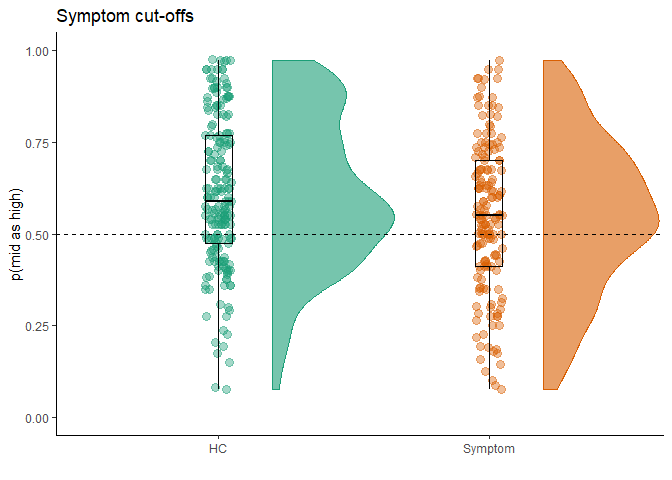
\includegraphics{OpenDataAnalysis_files/figure-latex/unnamed-chunk-9-1.pdf}

\begin{verbatim}
## [1] "The number of patients is N = 170"
\end{verbatim}

\begin{verbatim}
## [1] "The number of controls is N = 198"
\end{verbatim}

\begin{verbatim}
## 
##  Two Sample t-test
## 
## data:  Pmid by group
## t = 2.766, df = 349, p-value = 0.005976
## alternative hypothesis: true difference in means is not equal to 0
## 95 percent confidence interval:
##  0.01762747 0.10438403
## sample estimates:
##      mean in group HC mean in group Symptom 
##             0.6087543             0.5477486
\end{verbatim}

\begin{verbatim}
## [1] "The effect size of the Human group difference on p(mid as high) is d= 0.3"
\end{verbatim}

\begin{verbatim}
## 
##  Two Sample t-test
## 
## data:  driftrate by group
## t = 2.78, df = 349, p-value = 0.005731
## alternative hypothesis: true difference in means is not equal to 0
## 95 percent confidence interval:
##  0.001015933 0.005930341
## sample estimates:
##      mean in group HC mean in group Symptom 
##           0.006236747           0.002763610
\end{verbatim}

\begin{verbatim}
## [1] "The effect size of the Human group difference on driftrate is d= 0.3"
\end{verbatim}

\subsubsection{II) Latent mixture modelling
(data-driven)}\label{ii-latent-mixture-modelling-data-driven}

In a more data driven approach we ran an exploratory latent class
analysis based on the symptoms/traits (BDI, Age, IQ) that are predict
task performance in the regression. Notably we do not include task
performance in our class analysis so that classes are defined orthogonal
to task performance. Optimal class breakdown (N=5 classes) is plotted
below, but ordered by those with the higest postive bias based on the
symptom defined latent classes. We then defined the `symptomatic group'
as those with the lowest p(mid)as high score, whilst the control group
is those with the highest p(mid as high) score. The distributions of the
other latent classes are plotted in gray.

\begin{verbatim}
## fitting ...
## 
  |                                                                       
  |                                                                 |   0%
  |                                                                       
  |=                                                                |   1%
  |                                                                       
  |=                                                                |   2%
  |                                                                       
  |==                                                               |   2%
  |                                                                       
  |==                                                               |   3%
  |                                                                       
  |===                                                              |   4%
  |                                                                       
  |===                                                              |   5%
  |                                                                       
  |====                                                             |   6%
  |                                                                       
  |=====                                                            |   7%
  |                                                                       
  |=====                                                            |   8%
  |                                                                       
  |======                                                           |   9%
  |                                                                       
  |=======                                                          |  10%
  |                                                                       
  |=======                                                          |  11%
  |                                                                       
  |========                                                         |  12%
  |                                                                       
  |========                                                         |  13%
  |                                                                       
  |=========                                                        |  13%
  |                                                                       
  |=========                                                        |  14%
  |                                                                       
  |==========                                                       |  15%
  |                                                                       
  |==========                                                       |  16%
  |                                                                       
  |===========                                                      |  17%
  |                                                                       
  |============                                                     |  18%
  |                                                                       
  |============                                                     |  19%
  |                                                                       
  |=============                                                    |  20%
  |                                                                       
  |==============                                                   |  21%
  |                                                                       
  |==============                                                   |  22%
  |                                                                       
  |===============                                                  |  23%
  |                                                                       
  |===============                                                  |  24%
  |                                                                       
  |================                                                 |  24%
  |                                                                       
  |================                                                 |  25%
  |                                                                       
  |=================                                                |  26%
  |                                                                       
  |=================                                                |  27%
  |                                                                       
  |==================                                               |  28%
  |                                                                       
  |===================                                              |  29%
  |                                                                       
  |===================                                              |  30%
  |                                                                       
  |====================                                             |  31%
  |                                                                       
  |=====================                                            |  32%
  |                                                                       
  |=====================                                            |  33%
  |                                                                       
  |======================                                           |  34%
  |                                                                       
  |=======================                                          |  35%
  |                                                                       
  |========================                                         |  36%
  |                                                                       
  |========================                                         |  37%
  |                                                                       
  |=========================                                        |  38%
  |                                                                       
  |=========================                                        |  39%
  |                                                                       
  |==========================                                       |  39%
  |                                                                       
  |==========================                                       |  40%
  |                                                                       
  |===========================                                      |  41%
  |                                                                       
  |===========================                                      |  42%
  |                                                                       
  |============================                                     |  43%
  |                                                                       
  |=============================                                    |  44%
  |                                                                       
  |=============================                                    |  45%
  |                                                                       
  |==============================                                   |  46%
  |                                                                       
  |===============================                                  |  47%
  |                                                                       
  |===============================                                  |  48%
  |                                                                       
  |================================                                 |  49%
  |                                                                       
  |================================                                 |  50%
  |                                                                       
  |=================================                                |  50%
  |                                                                       
  |=================================                                |  51%
  |                                                                       
  |==================================                               |  52%
  |                                                                       
  |==================================                               |  53%
  |                                                                       
  |===================================                              |  54%
  |                                                                       
  |====================================                             |  55%
  |                                                                       
  |====================================                             |  56%
  |                                                                       
  |=====================================                            |  57%
  |                                                                       
  |======================================                           |  58%
  |                                                                       
  |======================================                           |  59%
  |                                                                       
  |=======================================                          |  60%
  |                                                                       
  |=======================================                          |  61%
  |                                                                       
  |========================================                         |  61%
  |                                                                       
  |========================================                         |  62%
  |                                                                       
  |=========================================                        |  63%
  |                                                                       
  |=========================================                        |  64%
  |                                                                       
  |==========================================                       |  65%
  |                                                                       
  |===========================================                      |  66%
  |                                                                       
  |============================================                     |  67%
  |                                                                       
  |============================================                     |  68%
  |                                                                       
  |=============================================                    |  69%
  |                                                                       
  |==============================================                   |  70%
  |                                                                       
  |==============================================                   |  71%
  |                                                                       
  |===============================================                  |  72%
  |                                                                       
  |================================================                 |  73%
  |                                                                       
  |================================================                 |  74%
  |                                                                       
  |=================================================                |  75%
  |                                                                       
  |=================================================                |  76%
  |                                                                       
  |==================================================               |  76%
  |                                                                       
  |==================================================               |  77%
  |                                                                       
  |===================================================              |  78%
  |                                                                       
  |===================================================              |  79%
  |                                                                       
  |====================================================             |  80%
  |                                                                       
  |=====================================================            |  81%
  |                                                                       
  |=====================================================            |  82%
  |                                                                       
  |======================================================           |  83%
  |                                                                       
  |=======================================================          |  84%
  |                                                                       
  |=======================================================          |  85%
  |                                                                       
  |========================================================         |  86%
  |                                                                       
  |========================================================         |  87%
  |                                                                       
  |=========================================================        |  87%
  |                                                                       
  |=========================================================        |  88%
  |                                                                       
  |==========================================================       |  89%
  |                                                                       
  |==========================================================       |  90%
  |                                                                       
  |===========================================================      |  91%
  |                                                                       
  |============================================================     |  92%
  |                                                                       
  |============================================================     |  93%
  |                                                                       
  |=============================================================    |  94%
  |                                                                       
  |==============================================================   |  95%
  |                                                                       
  |==============================================================   |  96%
  |                                                                       
  |===============================================================  |  97%
  |                                                                       
  |===============================================================  |  98%
  |                                                                       
  |================================================================ |  98%
  |                                                                       
  |================================================================ |  99%
  |                                                                       
  |=================================================================| 100%
\end{verbatim}

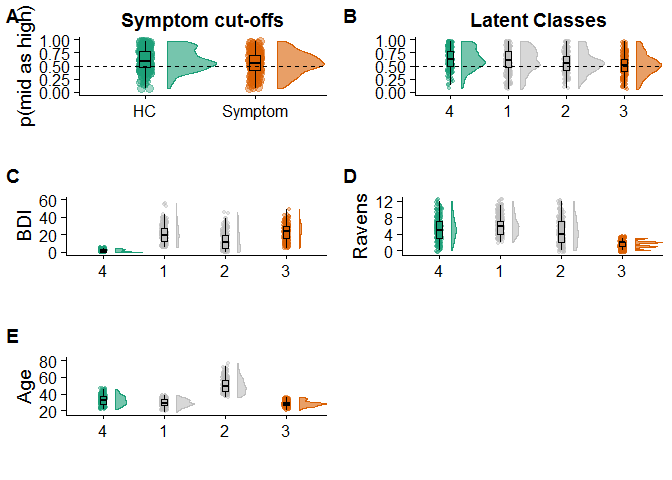
\includegraphics{OpenDataAnalysis_files/figure-latex/unnamed-chunk-10-1.pdf}

\begin{verbatim}
## ---------------------------------------------------- 
## Gaussian finite mixture model fitted by EM algorithm 
## ---------------------------------------------------- 
## 
## Mclust VVI (diagonal, varying volume and shape) model with 4 components: 
## 
##  log-likelihood   n df       BIC       ICL
##        -9629.49 994 27 -19445.33 -19841.74
## 
## Clustering table:
##   1   2   3   4 
## 219 233 266 276
\end{verbatim}

\begin{verbatim}
## 
##  Two Sample t-test
## 
## data:  Pmid by group
## t = -5.8731, df = 497, p-value = 7.836e-09
## alternative hypothesis: true difference in means is not equal to 0
## 95 percent confidence interval:
##  -0.13813301 -0.06887991
## sample estimates:
##      mean in group HC mean in group Symptom 
##             0.5310236             0.6345301
\end{verbatim}

\begin{verbatim}
## [1] "The effect size of the Human group difference on driftrate is d= 0.53"
\end{verbatim}

\begin{verbatim}
## 
##  Two Sample t-test
## 
## data:  BDI by group
## t = 32.016, df = 497, p-value < 2.2e-16
## alternative hypothesis: true difference in means is not equal to 0
## 95 percent confidence interval:
##  19.31422 21.83977
## sample estimates:
##      mean in group HC mean in group Symptom 
##             22.259398              1.682403
\end{verbatim}

\begin{verbatim}
## [1] "The effect size of the Human group difference is d= 2.87"
\end{verbatim}

\begin{verbatim}
## 
##  Two Sample t-test
## 
## data:  Age by group
## t = -10.506, df = 497, p-value < 2.2e-16
## alternative hypothesis: true difference in means is not equal to 0
## 95 percent confidence interval:
##  -5.246439 -3.593246
## sample estimates:
##      mean in group HC mean in group Symptom 
##              28.20677              32.62661
\end{verbatim}

\begin{verbatim}
## 
##  Two Sample t-test
## 
## data:  Ravens by group
## t = -20.409, df = 497, p-value < 2.2e-16
## alternative hypothesis: true difference in means is not equal to 0
## 95 percent confidence interval:
##  -4.137983 -3.411244
## sample estimates:
##      mean in group HC mean in group Symptom 
##              1.560150              5.334764
\end{verbatim}

\paragraph{Interpretation}\label{interpretation-4}

This approach identified 5 latent classes. Confirming our initial study,
the group with the highest mean depression scores are those with the
greatest negative bias, while those with the highest bias have very low
depression scores. Interestingly, the `symptomatic' latent class is also
particularly low IQ relative to the other classes. These results are
(highly!) exploratory and should be approached with caution, but they
perhaps suggest that IQ can protect against negative bias in depressed
individuals (which has been speculated in therapy research before). They
also provide predictions about the distributions of relevant variables
within those who may be currently or at risk of developping
clinically-relevant behavioural symptoms.

\subsubsection{Supplementary Analysis}\label{supplementary-analysis}

\subsubsection{Exploratory Factor Analysis of
questionnaires}\label{exploratory-factor-analysis-of-questionnaires}

The simple regression above, however, collapses across the individual
responses to the different items on the questionnaires and just uses
summary scores. However, it may be that there is a simpler underlying
structure to the data. For instance BDI and STAI are often highly
correlated - so may actually be measuring the same latent construct. In
this next section (inspired by Gillan et al 2016) we first run an
exploratory factor analysis on the individual items from the
questionnaires in an attempt to reduce the amount of latent variables.

\begin{Shaded}
\begin{Highlighting}[]
\NormalTok{###EFA}

\CommentTok{#Determine facrors using Cattell-Nelson-Gorsuch CNG Indices (claire's approach)}
\NormalTok{determinefactors <-}\StringTok{ }\KeywordTok{nCng}\NormalTok{(combineditemdata[}\DecValTok{44}\OperatorTok{:}\DecValTok{143}\NormalTok{], }\DataTypeTok{cor=}\OtherTok{TRUE}\NormalTok{, }\DataTypeTok{model=}\StringTok{"factors"}\NormalTok{)}
\CommentTok{#Do an EFA using N factors from CNG}
\NormalTok{efaQaires <-}\StringTok{ }\KeywordTok{fa}\NormalTok{(combineditemdata[}\DecValTok{44}\OperatorTok{:}\DecValTok{143}\NormalTok{], }\DataTypeTok{nfact =}\NormalTok{ determinefactors}\OperatorTok{$}\NormalTok{nFactors, }\DataTypeTok{rotate =} \StringTok{"geominQ"}\NormalTok{, }\DataTypeTok{fm =} \StringTok{"ml"}\NormalTok{)}

\NormalTok{efaQaires.loadmat <-}\StringTok{ }\KeywordTok{zapsmall}\NormalTok{(}\KeywordTok{matrix}\NormalTok{(}\KeywordTok{round}\NormalTok{(efaQaires}\OperatorTok{$}\NormalTok{loadings, }\DecValTok{2}\NormalTok{), }\DataTypeTok{nrow =} \DecValTok{100}\NormalTok{, }\DataTypeTok{ncol =} \DecValTok{3}\NormalTok{))}
\KeywordTok{rownames}\NormalTok{(efaQaires.loadmat) <-}\StringTok{ }\KeywordTok{names}\NormalTok{(combineditemdata[}\DecValTok{44}\OperatorTok{:}\DecValTok{143}\NormalTok{])}

\CommentTok{#heatmap}
\NormalTok{efaQairesdataf <-}\StringTok{ }\KeywordTok{data.frame}\NormalTok{(efaQaires.loadmat)}
\KeywordTok{row.names}\NormalTok{(efaQairesdataf) <-}\StringTok{ }\KeywordTok{gsub}\NormalTok{(}\StringTok{"_quantised"}\NormalTok{, }\StringTok{""}\NormalTok{, }\KeywordTok{row.names}\NormalTok{(efaQairesdataf))}
\KeywordTok{names}\NormalTok{(efaQairesdataf)<-}\KeywordTok{c}\NormalTok{(}\StringTok{"AnxDepression"}\NormalTok{,}\StringTok{"ObsessiveCompulsive"}\NormalTok{,}\StringTok{"Schizotypy"}\NormalTok{)}
\NormalTok{annotation <-}\StringTok{ }\KeywordTok{substr}\NormalTok{(}\KeywordTok{row.names}\NormalTok{(efaQairesdataf), }\DataTypeTok{start=}\DecValTok{1}\NormalTok{, }\DataTypeTok{stop=}\DecValTok{3}\NormalTok{)}
\NormalTok{annotationdf <-}\StringTok{ }\KeywordTok{data.frame}\NormalTok{(}\DataTypeTok{Questionnaire =}\NormalTok{ annotation)}
\KeywordTok{levels}\NormalTok{(annotationdf}\OperatorTok{$}\NormalTok{Questionnaire) <-}\StringTok{ }\KeywordTok{c}\NormalTok{(}\StringTok{'BDI'}\NormalTok{, }\StringTok{'OCIR'}\NormalTok{, }\StringTok{'STAI'}\NormalTok{, }\StringTok{'SZ'}\NormalTok{)}
\KeywordTok{rownames}\NormalTok{(annotationdf) <-}\StringTok{ }\KeywordTok{rownames}\NormalTok{(efaQairesdataf)}
\NormalTok{countqs <-}\StringTok{ }\KeywordTok{summary}\NormalTok{(annotationdf}\OperatorTok{$}\NormalTok{Questionnaire)}
\NormalTok{qbreaks <-}\StringTok{ }\KeywordTok{c}\NormalTok{(countqs[}\DecValTok{1}\NormalTok{], (countqs[}\DecValTok{1}\NormalTok{]}\OperatorTok{+}\NormalTok{countqs[}\DecValTok{2}\NormalTok{]), (countqs[}\DecValTok{1}\NormalTok{]}\OperatorTok{+}\NormalTok{countqs[}\DecValTok{2}\NormalTok{]}\OperatorTok{+}\NormalTok{countqs[}\DecValTok{4}\NormalTok{]) )}
\NormalTok{ancol =}\StringTok{ }\KeywordTok{list}\NormalTok{(}\DataTypeTok{Questionnaire =}\KeywordTok{c}\NormalTok{(}\DataTypeTok{BDI =}\StringTok{"lavenderblush4"}\NormalTok{, }\DataTypeTok{OCIR =}\StringTok{"darkolivegreen3"}\NormalTok{, }\DataTypeTok{STAI =}\StringTok{"plum3"}\NormalTok{,}\DataTypeTok{SZ =}\StringTok{"goldenrod1"}\NormalTok{))}

\NormalTok{heatmapplot <-}\StringTok{ }\KeywordTok{pheatmap}\NormalTok{(}
  \DataTypeTok{mat               =}\NormalTok{ efaQairesdataf,}
  \DataTypeTok{border_color      =} \OtherTok{NA}\NormalTok{,}
  \DataTypeTok{color             =} \KeywordTok{colorRampPalette}\NormalTok{(}\KeywordTok{c}\NormalTok{(}\StringTok{"darkblue"}\NormalTok{, }\StringTok{"white"}\NormalTok{, }\StringTok{"firebrick3"}\NormalTok{))(}\DecValTok{50}\NormalTok{),}
  \DataTypeTok{cellwidth         =} \DecValTok{70}\NormalTok{,}
  \DataTypeTok{cellheight        =} \DecValTok{3}\NormalTok{,}
  \DataTypeTok{show_colnames     =} \OtherTok{TRUE}\NormalTok{,}
  \DataTypeTok{show_rownames     =} \OtherTok{FALSE}\NormalTok{,}
  \DataTypeTok{drop_levels       =} \OtherTok{TRUE}\NormalTok{,}
  \DataTypeTok{fontsize          =} \DecValTok{14}\NormalTok{,}
  \DataTypeTok{main              =} \StringTok{"Factors"}\NormalTok{,}
  \DataTypeTok{treeheight_row    =} \DecValTok{0}\NormalTok{, }
  \DataTypeTok{treeheight_col    =} \DecValTok{0}\NormalTok{,}
  \DataTypeTok{cluster_rows      =} \OtherTok{FALSE}\NormalTok{,}
  \DataTypeTok{annotation_row    =}\NormalTok{ annotationdf,}
  \DataTypeTok{annotation_colors =}\NormalTok{ ancol,}
  \DataTypeTok{angle_col         =} \DecValTok{45}\NormalTok{,}
  \DataTypeTok{gaps_row          =}\NormalTok{ qbreaks,}
  \DataTypeTok{gaps_col          =} \KeywordTok{c}\NormalTok{(}\DecValTok{1}\NormalTok{,}\DecValTok{2}\NormalTok{),}
  \DataTypeTok{width             =} \DecValTok{20}\NormalTok{, }
    \DataTypeTok{height            =} \DecValTok{20}
\NormalTok{)}


\NormalTok{heatmapplot}
\end{Highlighting}
\end{Shaded}

\begin{center}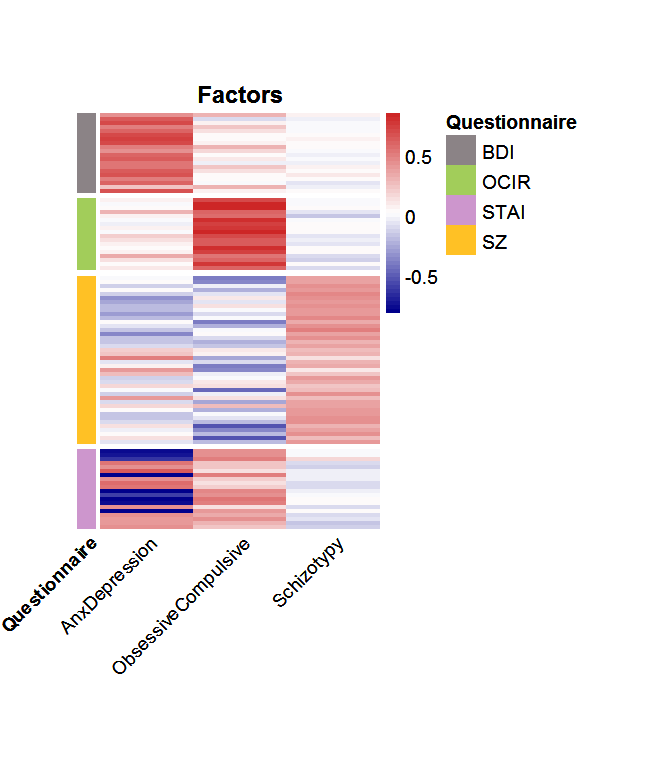
\includegraphics{OpenDataAnalysis_files/figure-latex/unnamed-chunk-11-1} \end{center}

\paragraph{Interpretation}\label{interpretation-5}

We Identify 3 latent factors using Cattell-Nelson-Gorsuch Indices (as in
Gillan et al.). One factor we name ``AnxDepression'' as it maps closely
onto the BDI and STAI , ``ObsessiveCompulsive'' which is a mix of the
OCIR and STAI (and not Schizotypy), and ``Schizotypy'' which loads
positively almost exclusively on the Schizotypy questionnaire.

\subsubsection{Exploratory Structural Equation Model using latent
factors}\label{exploratory-structural-equation-model-using-latent-factors}

We can now use these factor loadings in an Exploratory Structural
Equation Model (ESEM) and run the same regression as above but instead
of feeding in the summary questionnaire scores, we can create a latent
variable that represents each factor. Of note we use the `Robust maximum
likelihood' (MLR) estimator as it is robust to non-normality and the
individual items for the questionnaires are not continuous.

\begin{Shaded}
\begin{Highlighting}[]
\NormalTok{##ESEM which mimics regression - this takes the loadings from the EFA and uses them to weight the relationship between each questionnaire item and the three latent factors}
\NormalTok{terms <-}\StringTok{ }\KeywordTok{vector}\NormalTok{()}
\ControlFlowTok{for}\NormalTok{ (i }\ControlFlowTok{in} \DecValTok{1}\OperatorTok{:}\DecValTok{3}\NormalTok{) \{}
\NormalTok{  terms[i] <-}
\StringTok{    }\KeywordTok{paste0}\NormalTok{(}\StringTok{"F"}\NormalTok{,i,}\StringTok{"=~ "}\NormalTok{, }\KeywordTok{paste0}\NormalTok{(}\KeywordTok{c}\NormalTok{(efaQaires.loadmat[,i]), }\StringTok{"*"}\NormalTok{, }\KeywordTok{names}\NormalTok{(efaQaires.loadmat[,}\DecValTok{1}\NormalTok{]), }\DataTypeTok{collapse =} \StringTok{"+"}\NormalTok{))}
\NormalTok{\}}

\NormalTok{efaQaires.esem <-}\StringTok{ }\KeywordTok{paste}\NormalTok{(terms, }\DataTypeTok{collapse =} \StringTok{"}\CharTok{\textbackslash{}n}\StringTok{"}\NormalTok{)}
\NormalTok{##adding the regression and covariances to match the original regression analysis}
\NormalTok{terms[}\DecValTok{4}\NormalTok{] <-}\StringTok{ "propmedhigh ~ spreadsheet + Ravens + Age + GenderMF + F1 + F2 + F3"}
\NormalTok{##adding residual correlations}
\NormalTok{terms[}\DecValTok{5}\NormalTok{] <-}\StringTok{ "spreadsheet ~~ Ravens + Age + GenderMF + F1 + F2 + F3"}
\NormalTok{terms[}\DecValTok{6}\NormalTok{] <-}\StringTok{ "Ravens ~~ Age  + GenderMF + F1 + F2 + F3"}
\NormalTok{terms[}\DecValTok{7}\NormalTok{] <-}\StringTok{ "Age ~~  GenderMF + F1 + F2 + F3"}
\NormalTok{terms[}\DecValTok{8}\NormalTok{] <-}\StringTok{ "GenderMF ~~ F1 + F2 + F3"}
\NormalTok{terms[}\DecValTok{9}\NormalTok{] <-}\StringTok{ "F1 ~~ F2 + F3"}
\NormalTok{terms[}\DecValTok{10}\NormalTok{] <-}\StringTok{ "F2 ~~ F3"}

\NormalTok{semFactorsMatch <-}\StringTok{ }\KeywordTok{paste}\NormalTok{(terms, }\DataTypeTok{collapse =} \StringTok{"}\CharTok{\textbackslash{}n}\StringTok{"}\NormalTok{)}

\CommentTok{#Fit the model (this takes a while!)}
\NormalTok{fititem.factors <-}\StringTok{ }\KeywordTok{sem}\NormalTok{(semFactorsMatch, }\DataTypeTok{data=}\NormalTok{combineditemdata, }\DataTypeTok{meanstructure=}\OtherTok{TRUE}\NormalTok{,  }\DataTypeTok{estimator =} \StringTok{"MLR"}\NormalTok{)}

\CommentTok{#This plots loads of fit indices, but we are mostly intersted in the regression}
\KeywordTok{summary}\NormalTok{(fititem.factors, }\DataTypeTok{standardized=}\OtherTok{TRUE}\NormalTok{, }\DataTypeTok{rsquare=}\NormalTok{F, }\DataTypeTok{fit.measures=}\NormalTok{F)}
\end{Highlighting}
\end{Shaded}

\begin{verbatim}
## lavaan 0.6-3 ended normally after 267 iterations
## 
##   Optimization method                           NLMINB
##   Number of free parameters                        241
## 
##                                                   Used       Total
##   Number of observations                           990        1066
## 
##   Estimator                                         ML      Robust
##   Model Fit Test Statistic                   19555.630   17207.926
##   Degrees of freedom                              5429        5429
##   P-value (Chi-square)                           0.000       0.000
##   Scaling correction factor                                  1.136
##     for the Yuan-Bentler correction (Mplus variant)
## 
## Parameter Estimates:
## 
##   Information                                 Observed
##   Observed information based on                Hessian
##   Standard Errors                   Robust.huber.white
## 
## Latent Variables:
##                    Estimate  Std.Err  z-value  P(>|z|)   Std.lv  Std.all
##   F1 =~                                                                 
##     BDI_Attrctv_qn    0.620                               0.540    0.595
##     BDI_Blam_qntsd    0.680                               0.592    0.677
##     BDI_Cry_quntsd    0.470                               0.409    0.465
##     BDI_Dcsns_qnts    0.590                               0.513    0.587
##     BDI_Dsppntmnt_    0.690                               0.600    0.682
##     BDI_Falr_qntsd    0.710                               0.618    0.684
##     BDI_Futr_qntsd    0.670                               0.583    0.658
##     BDI_Glty_qntsd    0.490                               0.426    0.481
##     BDI_Hlth_qntsd    0.430                               0.374    0.463
##     BDI_Intrs_I_P_    0.590                               0.513    0.584
##     BDI_Irrttd_qnt    0.600                               0.522    0.588
##     BDI_Libd_qntsd    0.540                               0.470    0.540
##     BDI_Pnshd_qnts    0.500                               0.435    0.467
##     BDI_Sad_quntsd    0.620                               0.540    0.647
##     BDI_Stsfctn_qn    0.640                               0.557    0.606
##     BDI_Slep_qntsd    0.480                               0.418    0.469
##     BDI_Tird_qntsd    0.570                               0.496    0.586
##     BDI_wght_qntsd    0.220                               0.191    0.253
##     BDI_Work_qntsd    0.650                               0.566    0.645
##     OCIR_1_quantsd    0.070                               0.061    0.053
##     OCIR_10_quntsd    0.000                               0.000    0.000
##     OCIR_11_quntsd    0.020                               0.017    0.015
##     OCIR_12_quntsd    0.300                               0.261    0.231
##     OCIR_13_quntsd    0.070                               0.061    0.054
##     OCIR_14_quntsd    0.010                               0.009    0.007
##     OCIR_15_quntsd   -0.040                              -0.035   -0.029
##     OCIR_16_quntsd    0.050                               0.044    0.038
##     OCIR_17_quntsd   -0.010                              -0.009   -0.008
##     OCIR_18_quntsd    0.210                               0.183    0.162
##     OCIR_2_quantsd    0.120                               0.104    0.088
##     OCIR_3_quantsd    0.060                               0.052    0.045
##     OCIR_4_quantsd    0.020                               0.017    0.015
##     OCIR_5_quantsd    0.060                               0.052    0.045
##     OCIR_6_quantsd    0.350                               0.305    0.273
##     OCIR_7_quantsd    0.110                               0.096    0.087
##     OCIR_8_quantsd    0.040                               0.035    0.029
##     OCIR_9_quantsd    0.110                               0.096    0.083
##     SZ_1_quantised    0.000                               0.000    0.000
##     SZ_10_quantisd    0.020                               0.017    0.035
##     SZ_11_quantisd   -0.140                              -0.122   -0.249
##     SZ_12_quantisd    0.050                               0.044    0.090
##     SZ_13_quantisd   -0.130                              -0.113   -0.234
##     SZ_14_quantisd   -0.340                              -0.296   -0.556
##     SZ_15_quantisd   -0.280                              -0.244   -0.463
##     SZ_16_quantisd   -0.220                              -0.191   -0.374
##     SZ_17_quantisd   -0.230                              -0.200   -0.393
##     SZ_18_quantisd   -0.290                              -0.252   -0.472
##     SZ_19_quantisd   -0.190                              -0.165   -0.332
##     SZ_2_quantised    0.040                               0.035    0.065
##     SZ_20_quantisd   -0.070                              -0.061   -0.130
##     SZ_21_quantisd   -0.190                              -0.165   -0.335
##     SZ_22_quantisd   -0.370                              -0.322   -0.583
##     SZ_23_quantisd   -0.160                              -0.139   -0.283
##     SZ_24_quantisd   -0.160                              -0.139   -0.254
##     SZ_25_quantisd   -0.090                              -0.078   -0.156
##     SZ_26_quantisd    0.210                               0.183    0.336
##     SZ_27_quantisd    0.220                               0.191    0.359
##     SZ_28_quantisd    0.490                               0.426    0.727
##     SZ_29_quantisd   -0.070                              -0.061   -0.124
##     SZ_3_quantised    0.080                               0.070    0.137
##     SZ_30_quantisd    0.390                               0.339    0.600
##     SZ_31_quantisd    0.270                               0.235    0.463
##     SZ_32_quantisd   -0.150                              -0.131   -0.264
##     SZ_33_quantisd   -0.130                              -0.113   -0.232
##     SZ_34_quantisd    0.170                               0.148    0.274
##     SZ_35_quantisd    0.000                               0.000    0.000
##     SZ_36_quantisd   -0.150                              -0.131   -0.266
##     SZ_37_quantisd    0.380                               0.331    0.524
##     SZ_38_quantisd   -0.090                              -0.078   -0.152
##     SZ_39_quantisd    0.140                               0.122    0.202
##     SZ_4_quantised    0.020                               0.017    0.037
##     SZ_40_quantisd   -0.160                              -0.139   -0.280
##     SZ_41_quantisd   -0.160                              -0.139   -0.283
##     SZ_42_quantisd   -0.100                              -0.087   -0.170
##     SZ_5_quantised    0.140                               0.122    0.208
##     SZ_6_quantised   -0.020                              -0.017   -0.033
##     SZ_7_quantised    0.020                               0.017    0.036
##     SZ_8_quantised    0.130                               0.113    0.186
##     SZ_9_quantised   -0.070                              -0.061   -0.123
##     STAI2_Clm_qnts   -0.770                              -0.670   -0.769
##     STAI2_Cntnt_qn   -0.740                              -0.644   -0.737
##     STAI2_Dscns_qn   -0.640                              -0.557   -0.643
##     STAI2_Dffclts_    0.540                               0.470    0.508
##     STAI2_DsppntS_    0.440                               0.383    0.420
##     STAI2_Flr_qnts    0.640                               0.557    0.605
##     STAI2_Hppy_qnt   -0.810                              -0.705   -0.807
##     STAI2_HppyOth_    0.420                               0.365    0.376
##     STAI2_Indqt_qn    0.580                               0.505    0.542
##     STAI2_Nrvs_qnt    0.540                               0.470    0.519
##     STAI2_Plsnt_qn   -0.820                              -0.714   -0.847
##     STAI2_Rstd_qnt   -0.610                              -0.531   -0.607
##     STAI2_StsfdSl_   -0.800                              -0.696   -0.789
##     STAI2_Scr_qnts   -0.770                              -0.670   -0.756
##     STAI2_SlfCnfd_    0.440                               0.383    0.387
##     STAI2_Stdy_qnt   -0.790                              -0.687   -0.800
##     STAI2_Tnsn_qnt    0.450                               0.392    0.422
##     STAI2_Thghts_q    0.380                               0.331    0.366
##     STAI2_UnmprtT_    0.400                               0.348    0.384
##     STAI2_Wrry_qnt    0.450                               0.392    0.417
##     STAI_Anxs_qnts    0.450                               0.392    0.407
##   F2 =~                                                                 
##     BDI_Attrctv_qn   -0.070                              -0.067   -0.074
##     BDI_Blam_qntsd    0.070                               0.067    0.076
##     BDI_Cry_quntsd    0.240                               0.229    0.260
##     BDI_Dcsns_qnts    0.140                               0.134    0.153
##     BDI_Dsppntmnt_    0.060                               0.057    0.065
##     BDI_Falr_qntsd    0.060                               0.057    0.063
##     BDI_Futr_qntsd    0.090                               0.086    0.097
##     BDI_Glty_qntsd    0.300                               0.287    0.323
##     BDI_Hlth_qntsd    0.170                               0.162    0.201
##     BDI_Intrs_I_P_    0.070                               0.067    0.076
##     BDI_Irrttd_qnt    0.130                               0.124    0.140
##     BDI_Libd_qntsd   -0.030                              -0.029   -0.033
##     BDI_Pnshd_qnts    0.240                               0.229    0.246
##     BDI_Sad_quntsd    0.140                               0.134    0.160
##     BDI_Stsfctn_qn    0.070                               0.067    0.073
##     BDI_Slep_qntsd    0.060                               0.057    0.064
##     BDI_Tird_qntsd    0.010                               0.010    0.011
##     BDI_wght_qntsd    0.290                               0.277    0.367
##     BDI_Work_qntsd    0.080                               0.076    0.087
##     OCIR_1_quantsd    0.710                               0.678    0.593
##     OCIR_10_quntsd    0.860                               0.821    0.740
##     OCIR_11_quntsd    0.840                               0.802    0.699
##     OCIR_12_quntsd    0.620                               0.592    0.525
##     OCIR_13_quntsd    0.580                               0.554    0.487
##     OCIR_14_quntsd    0.830                               0.793    0.677
##     OCIR_15_quntsd    0.740                               0.707    0.592
##     OCIR_16_quntsd    0.790                               0.755    0.654
##     OCIR_17_quntsd    0.860                               0.821    0.713
##     OCIR_18_quntsd    0.710                               0.678    0.601
##     OCIR_2_quantsd    0.640                               0.611    0.516
##     OCIR_3_quantsd    0.650                               0.621    0.540
##     OCIR_4_quantsd    0.830                               0.793    0.692
##     OCIR_5_quantsd    0.770                               0.735    0.635
##     OCIR_6_quantsd    0.550                               0.525    0.471
##     OCIR_7_quantsd    0.610                               0.583    0.531
##     OCIR_8_quantsd    0.800                               0.764    0.645
##     OCIR_9_quantsd    0.630                               0.602    0.522
##     SZ_1_quantised   -0.390                              -0.373   -0.668
##     SZ_10_quantisd   -0.350                              -0.334   -0.667
##     SZ_11_quantisd   -0.040                              -0.038   -0.078
##  [ reached getOption("max.print") -- omitted 161 rows ]
## 
## Regressions:
##                    Estimate  Std.Err  z-value  P(>|z|)   Std.lv  Std.all
##   propmedhigh ~                                                         
##     spreadsheet       0.006    0.002    2.767    0.006    0.006    0.086
##     Ravens            0.010    0.002    4.339    0.000    0.010    0.145
##     Age              -0.003    0.001   -3.900    0.000   -0.003   -0.124
##     GenderMF         -0.005    0.013   -0.388    0.698   -0.005   -0.012
##     F1               -0.023    0.009   -2.624    0.009   -0.020   -0.097
##     F2               -0.009    0.009   -1.011    0.312   -0.008   -0.040
##     F3                0.006    0.018    0.309    0.757    0.002    0.011
## 
## Covariances:
##                    Estimate  Std.Err  z-value  P(>|z|)   Std.lv  Std.all
##   spreadsheet ~~                                                        
##     Ravens           -0.395    0.280   -1.408    0.159   -0.395   -0.045
##     Age               1.278    0.974    1.312    0.190    1.278    0.042
##     GenderMF          0.059    0.047    1.264    0.206    0.059    0.040
##   F1 ~~                                                                 
##     spreadsheet      -0.012    0.084   -0.143    0.886   -0.014   -0.005
##   F2 ~~                                                                 
##     spreadsheet       0.090    0.093    0.968    0.333    0.094    0.031
##   F3 ~~                                                                 
##     spreadsheet      -0.021    0.043   -0.497    0.619   -0.052   -0.017
##   Ravens ~~                                                             
##     Age               2.696    0.986    2.734    0.006    2.696    0.090
##     GenderMF         -0.070    0.046   -1.528    0.126   -0.070   -0.048
##   F1 ~~                                                                 
##     Ravens           -0.410    0.080   -5.142    0.000   -0.471   -0.160
##   F2 ~~                                                                 
##     Ravens           -0.983    0.086  -11.432    0.000   -1.029   -0.349
##   F3 ~~                                                                 
##     Ravens           -0.073    0.043   -1.702    0.089   -0.176   -0.060
##   Age ~~                                                                
##     GenderMF         -0.061    0.160   -0.379    0.705   -0.061   -0.012
##   F1 ~~                                                                 
##     Age              -2.154    0.310   -6.941    0.000   -2.476   -0.242
##   F2 ~~                                                                 
##     Age              -3.192    0.281  -11.367    0.000   -3.341   -0.327
##   F3 ~~                                                                 
##     Age               0.024    0.131    0.184    0.854    0.058    0.006
##   F1 ~~                                                                 
##     GenderMF          0.014    0.014    0.992    0.321    0.016    0.032
##   F2 ~~                                                                 
##     GenderMF          0.040    0.015    2.645    0.008    0.041    0.084
##   F3 ~~                                                                 
##     GenderMF          0.004    0.007    0.627    0.531    0.011    0.022
##   F1 ~~                                                                 
##     F2                0.386    0.022   17.289    0.000    0.465    0.465
##     F3               -0.070    0.012   -6.097    0.000   -0.196   -0.196
##   F2 ~~                                                                 
##     F3               -0.007    0.016   -0.474    0.635   -0.019   -0.019
## 
## Intercepts:
##                    Estimate  Std.Err  z-value  P(>|z|)   Std.lv  Std.all
##    .BDI_Attrctv_qn    1.851    0.030   61.691    0.000    1.851    2.042
##    .BDI_Blam_qntsd    1.880    0.028   67.386    0.000    1.880    2.149
##    .BDI_Cry_quntsd    1.608    0.028   57.827    0.000    1.608    1.827
##    .BDI_Dcsns_qnts    1.730    0.028   61.375    0.000    1.730    1.979
##    .BDI_Dsppntmnt_    1.838    0.028   65.497    0.000    1.838    2.087
##    .BDI_Falr_qntsd    1.838    0.029   63.321    0.000    1.838    2.034
##    .BDI_Futr_qntsd    1.865    0.028   65.850    0.000    1.865    2.103
##    .BDI_Glty_qntsd    1.649    0.027   61.055    0.000    1.649    1.862
##    .BDI_Hlth_qntsd    1.691    0.025   68.835    0.000    1.691    2.094
##    .BDI_Intrs_I_P_    1.868    0.029   64.901    0.000    1.868    2.125
##    .BDI_Irrttd_qnt    1.867    0.028   66.237    0.000    1.867    2.103
##    .BDI_Libd_qntsd    1.694    0.028   60.268    0.000    1.694    1.946
##    .BDI_Pnshd_qnts    1.660    0.030   56.017    0.000    1.660    1.780
##    .BDI_Sad_quntsd    1.682    0.025   68.386    0.000    1.682    2.017
##    .BDI_Stsfctn_qn    1.836    0.030   62.084    0.000    1.836    1.998
##    .BDI_Slep_qntsd    1.836    0.029   64.377    0.000    1.836    2.060
##    .BDI_Tird_qntsd    1.914    0.027   70.442    0.000    1.914    2.263
##    .BDI_wght_qntsd    1.374    0.023   60.476    0.000    1.374    1.819
##    .BDI_Work_qntsd    1.788    0.027   65.179    0.000    1.788    2.040
##    .OCIR_1_quantsd    2.392    0.041   58.871    0.000    2.392    2.090
##    .OCIR_10_quntsd    1.991    0.041   48.896    0.000    1.991    1.793
##    .OCIR_11_quntsd    2.203    0.041   53.208    0.000    2.203    1.918
##    .OCIR_12_quntsd    2.316    0.041   56.177    0.000    2.316    2.052
##    .OCIR_13_quntsd    2.424    0.040   60.536    0.000    2.424    2.130
##    .OCIR_14_quntsd    2.186    0.043   51.180    0.000    2.186    1.865
##    .OCIR_15_quntsd    2.398    0.041   58.107    0.000    2.398    2.010
##    .OCIR_16_quntsd    2.127    0.042   51.049    0.000    2.127    1.844
##    .OCIR_17_quntsd    2.178    0.043   51.149    0.000    2.178    1.890
##    .OCIR_18_quntsd    2.231    0.042   52.896    0.000    2.231    1.977
##    .OCIR_2_quantsd    2.642    0.041   64.103    0.000    2.642    2.229
##    .OCIR_3_quantsd    2.466    0.040   61.560    0.000    2.466    2.143
##    .OCIR_4_quantsd    2.220    0.041   54.210    0.000    2.220    1.938
##    .OCIR_5_quantsd    2.155    0.041   52.331    0.000    2.155    1.859
##    .OCIR_6_quantsd    2.380    0.041   58.370    0.000    2.380    2.132
##    .OCIR_7_quantsd    2.189    0.039   55.883    0.000    2.189    1.995
##    .OCIR_8_quantsd    2.266    0.042   53.357    0.000    2.266    1.912
##    .OCIR_9_quantsd    2.520    0.040   62.668    0.000    2.520    2.185
##    .SZ_1_quantised    1.615    0.015  104.447    0.000    1.615    2.896
##    .SZ_10_quantisd    1.768    0.013  131.700    0.000    1.768    3.524
##    .SZ_11_quantisd    1.579    0.016  100.608    0.000    1.579    3.231
##    .SZ_12_quantisd    1.645    0.015  108.227    0.000    1.645    3.398
##    .SZ_13_quantisd    1.583    0.016  101.001    0.000    1.583    3.279
##    .SZ_14_quantisd    1.522    0.016   95.886    0.000    1.522    2.859
##    .SZ_15_quantisd    1.537    0.016   97.016    0.000    1.537    2.924
##    .SZ_16_quantisd    1.512    0.016   95.184    0.000    1.512    2.951
##    .SZ_17_quantisd    1.561    0.016   98.936    0.000    1.561    3.063
##    .SZ_18_quantisd    1.583    0.016  101.001    0.000    1.583    2.958
##    .SZ_19_quantisd    1.555    0.016   98.413    0.000    1.555    3.120
##    .SZ_2_quantised    1.612    0.015  104.099    0.000    1.612    2.998
##    .SZ_20_quantisd    1.710    0.014  118.592    0.000    1.710    3.647
##    .SZ_21_quantisd    1.572    0.016   99.939    0.000    1.572    3.186
##    .SZ_22_quantisd    1.554    0.016   98.327    0.000    1.554    2.815
##    .SZ_23_quantisd    1.598    0.016  102.547    0.000    1.598    3.250
##    .SZ_24_quantisd    1.595    0.016  102.228    0.000    1.595    2.909
##    .SZ_25_quantisd    1.571    0.016   99.846    0.000    1.571    3.120
##    .SZ_26_quantisd    1.305    0.015   89.183    0.000    1.305    2.397
##    .SZ_27_quantisd    1.296    0.015   89.329    0.000    1.296    2.431
##    .SZ_28_quantisd    1.386    0.015   89.575    0.000    1.386    2.362
##    .SZ_29_quantisd    1.585    0.016  101.200    0.000    1.585    3.236
##    .SZ_3_quantised    1.740    0.014  124.906    0.000    1.740    3.418
##    .SZ_30_quantisd    1.419    0.016   90.497    0.000    1.419    2.509
##    .SZ_31_quantisd    1.289    0.014   89.474    0.000    1.289    2.541
##    .SZ_32_quantisd    1.577    0.016  100.414    0.000    1.577    3.189
##    .SZ_33_quantisd    1.368    0.015   89.248    0.000    1.368    2.804
##    .SZ_34_quantisd    1.290    0.014   89.452    0.000    1.290    2.390
##    .SZ_35_quantisd    1.774    0.013  133.384    0.000    1.774    3.018
##    .SZ_36_quantisd    1.551    0.016   98.073    0.000    1.551    3.165
##    .SZ_37_quantisd    1.302    0.015   89.227    0.000    1.302    2.064
##    .SZ_38_quantisd    1.693    0.015  115.476    0.000    1.693    3.280
##    .SZ_39_quantisd    1.290    0.014   89.452    0.000    1.290    2.135
##    .SZ_4_quantised    1.690    0.015  114.957    0.000    1.690    3.577
##    .SZ_40_quantisd    1.577    0.016  100.414    0.000    1.577    3.172
##    .SZ_41_quantisd    1.570    0.016   99.753    0.000    1.570    3.188
##    .SZ_42_quantisd    1.559    0.016   98.760    0.000    1.559    3.049
##    .SZ_5_quantised    1.725    0.014  121.607    0.000    1.725    2.940
##    .SZ_6_quantised    1.715    0.014  119.568    0.000    1.715    3.252
##    .SZ_7_quantised    1.580    0.016  100.705    0.000    1.580    3.260
##    .SZ_8_quantised    1.714    0.014  119.370    0.000    1.714    2.820
##    .SZ_9_quantised    1.620    0.015  105.037    0.000    1.620    3.269
##    .STAI2_Clm_qnts    2.697    0.029   92.505    0.000    2.697    3.094
##    .STAI2_Cntnt_qn    2.684    0.029   92.224    0.000    2.684    3.070
##    .STAI2_Dscns_qn    2.654    0.029   91.842    0.000    2.654    3.065
##    .STAI2_Dffclts_    2.204    0.031   72.065    0.000    2.204    2.382
##    .STAI2_DsppntS_    2.194    0.030   73.103    0.000    2.194    2.404
##    .STAI2_Flr_qnts    2.026    0.030   66.523    0.000    2.026    2.199
##    .STAI2_Hppy_qnt    2.725    0.029   92.690    0.000    2.725    3.121
##    .STAI2_HppyOth_    2.491    0.032   78.398    0.000    2.491    2.562
##    .STAI2_Indqt_qn    2.172    0.031   69.873    0.000    2.172    2.332
##    .STAI2_Nrvs_qnt    2.206    0.030   74.217    0.000    2.206    2.434
##    .STAI2_Plsnt_qn    2.727    0.027  100.458    0.000    2.727    3.239
##    .STAI2_Rstd_qnt    2.469    0.028   86.925    0.000    2.469    2.823
##    .STAI2_StsfdSl_    2.610    0.031   84.756    0.000    2.610    2.957
##    .STAI2_Scr_qnts    2.716    0.030   89.572    0.000    2.716    3.063
##    .STAI2_SlfCnfd_    2.395    0.033   73.220    0.000    2.395    2.419
##    .STAI2_Stdy_qnt    2.767    0.029   96.893    0.000    2.767    3.219
##    .STAI2_Tnsn_qnt    2.218    0.031   72.603    0.000    2.218    2.389
##    .STAI2_Thghts_q    1.960    0.029   68.317    0.000    1.960    2.167
##    .STAI2_UnmprtT_    2.199    0.030   72.575    0.000    2.199    2.424
##    .STAI2_Wrry_qnt    2.266    0.031   72.806    0.000    2.266    2.415
##    .STAI_Anxs_qnts    2.136    0.032   67.610    0.000    2.136    2.223
##    .propmedhigh       0.601    0.027   21.984    0.000    0.601    2.870
##     spreadsheet       3.982    0.095   41.762    0.000    3.982    1.327
##     Ravens            4.458    0.094   47.626    0.000    4.458    1.514
##     Age              34.293    0.325  105.506    0.000   34.293    3.353
##     GenderMF          0.590    0.016   37.736    0.000    0.590    1.199
##     F1                0.000                               0.000    0.000
##     F2                0.000                               0.000    0.000
##     F3                0.000                               0.000    0.000
## 
## Variances:
##                    Estimate  Std.Err  z-value  P(>|z|)   Std.lv  Std.all
##    .BDI_Attrctv_qn    0.555    0.027   20.415    0.000    0.555    0.675
##    .BDI_Blam_qntsd    0.372    0.020   18.704    0.000    0.372    0.486
##    .BDI_Cry_quntsd    0.466    0.028   16.465    0.000    0.466    0.602
##    .BDI_Dcsns_qnts    0.417    0.022   18.928    0.000    0.417    0.545
##    .BDI_Dsppntmnt_    0.382    0.021   18.076    0.000    0.382    0.492
##    .BDI_Falr_qntsd    0.403    0.021   19.317    0.000    0.403    0.494
##    .BDI_Futr_qntsd    0.393    0.021   18.722    0.000    0.393    0.500
##    .BDI_Glty_qntsd    0.408    0.022   18.337    0.000    0.408    0.520
##    .BDI_Hlth_qntsd    0.427    0.021   19.988    0.000    0.427    0.655
##    .BDI_Intrs_I_P_    0.468    0.024   19.789    0.000    0.468    0.606
##    .BDI_Irrttd_qnt    0.439    0.021   20.558    0.000    0.439    0.557
##    .BDI_Libd_qntsd    0.545    0.029   18.813    0.000    0.545    0.719
##    .BDI_Pnshd_qnts    0.537    0.031   17.148    0.000    0.537    0.617
##    .BDI_Sad_quntsd    0.320    0.019   16.896    0.000    0.320    0.460
##    .BDI_Stsfctn_qn    0.500    0.026   19.209    0.000    0.500    0.592
##    .BDI_Slep_qntsd    0.594    0.028   21.251    0.000    0.594    0.747
##    .BDI_Tird_qntsd    0.459    0.023   20.059    0.000    0.459    0.641
##    .BDI_wght_qntsd    0.405    0.029   14.015    0.000    0.405    0.711
##    .BDI_Work_qntsd    0.403    0.020   20.155    0.000    0.403    0.525
##    .OCIR_1_quantsd    0.807    0.037   22.069    0.000    0.807    0.617
##    .OCIR_10_quntsd    0.558    0.034   16.194    0.000    0.558    0.453
##    .OCIR_11_quntsd    0.662    0.037   17.861    0.000    0.662    0.502
##    .OCIR_12_quntsd    0.710    0.032   21.876    0.000    0.710    0.557
##    .OCIR_13_quntsd    0.947    0.043   22.104    0.000    0.947    0.731
##    .OCIR_14_quntsd    0.738    0.043   17.077    0.000    0.738    0.538
##    .OCIR_15_quntsd    0.946    0.048   19.654    0.000    0.946    0.664
##    .OCIR_16_quntsd    0.730    0.041   17.883    0.000    0.730    0.548
##    .OCIR_17_quntsd    0.660    0.038   17.356    0.000    0.660    0.497
##    .OCIR_18_quntsd    0.664    0.034   19.238    0.000    0.664    0.521
##    .OCIR_2_quantsd    0.961    0.039   24.461    0.000    0.961    0.684
##    .OCIR_3_quantsd    0.905    0.043   20.819    0.000    0.905    0.683
##    .OCIR_4_quantsd    0.671    0.037   18.375    0.000    0.671    0.511
##    .OCIR_5_quantsd    0.764    0.044   17.253    0.000    0.764    0.569
##    .OCIR_6_quantsd    0.723    0.032   22.511    0.000    0.723    0.581
##    .OCIR_7_quantsd    0.797    0.038   21.000    0.000    0.797    0.662
##    .OCIR_8_quantsd    0.795    0.042   18.805    0.000    0.795    0.566
##    .OCIR_9_quantsd    0.904    0.042   21.668    0.000    0.904    0.679
##    .SZ_1_quantised    0.149    0.008   18.601    0.000    0.149    0.480
##    .SZ_10_quantisd    0.119    0.006   18.757    0.000    0.119    0.475
##    .SZ_11_quantisd    0.178    0.006   31.630    0.000    0.178    0.745
##    .SZ_12_quantisd    0.169    0.007   25.862    0.000    0.169    0.720
##    .SZ_13_quantisd    0.165    0.005   30.114    0.000    0.165    0.706
##    .SZ_14_quantisd    0.163    0.007   22.702    0.000    0.163    0.574
##    .SZ_15_quantisd    0.162    0.007   24.800    0.000    0.162    0.588
##    .SZ_16_quantisd    0.190    0.006   29.799    0.000    0.190    0.722
##    .SZ_17_quantisd    0.177    0.006   28.241    0.000    0.177    0.683
##    .SZ_18_quantisd    0.154    0.007   23.008    0.000    0.154    0.539
##    .SZ_19_quantisd    0.177    0.006   29.102    0.000    0.177    0.713
##    .SZ_2_quantised    0.154    0.008   20.034    0.000    0.154    0.531
##    .SZ_20_quantisd    0.123    0.006   21.571    0.000    0.123    0.557
##    .SZ_21_quantisd    0.164    0.006   27.710    0.000    0.164    0.674
##    .SZ_22_quantisd    0.163    0.007   22.434    0.000    0.163    0.535
##    .SZ_23_quantisd    0.165    0.006   27.641    0.000    0.165    0.682
##    .SZ_24_quantisd    0.178    0.008   23.352    0.000    0.178    0.593
##    .SZ_25_quantisd    0.187    0.006   30.150    0.000    0.187    0.737
##    .SZ_26_quantisd    0.226    0.009   26.341    0.000    0.226    0.764
##    .SZ_27_quantisd    0.218    0.009   24.766    0.000    0.218    0.766
##    .SZ_28_quantisd    0.206    0.009   22.723    0.000    0.206    0.597
##    .SZ_29_quantisd    0.207    0.005   40.205    0.000    0.207    0.864
##    .SZ_3_quantised    0.135    0.007   17.980    0.000    0.135    0.519
##    .SZ_30_quantisd    0.208    0.008   24.841    0.000    0.208    0.651
##    .SZ_31_quantisd    0.206    0.008   25.839    0.000    0.206    0.799
##    .SZ_32_quantisd    0.193    0.006   33.945    0.000    0.193    0.791
##    .SZ_33_quantisd    0.204    0.005   37.434    0.000    0.204    0.857
##    .SZ_34_quantisd    0.222    0.009   25.307    0.000    0.222    0.761
##    .SZ_35_quantisd    0.147    0.009   17.302    0.000    0.147    0.427
##    .SZ_36_quantisd    0.178    0.006   31.427    0.000    0.178    0.741
##    .SZ_37_quantisd    0.232    0.010   22.767    0.000    0.232    0.584
##    .SZ_38_quantisd    0.144    0.007   21.426    0.000    0.144    0.541
##    .SZ_39_quantisd    0.235    0.011   21.095    0.000    0.235    0.643
##    .SZ_4_quantised    0.146    0.007   22.383    0.000    0.146    0.656
##    .SZ_40_quantisd    0.193    0.006   32.916    0.000    0.193    0.780
##    .SZ_41_quantisd    0.175    0.006   30.163    0.000    0.175    0.723
##    .SZ_42_quantisd    0.165    0.007   25.171    0.000    0.165    0.630
##    .SZ_5_quantised    0.135    0.008   16.056    0.000    0.135    0.391
##    .SZ_6_quantised    0.137    0.007   19.494    0.000    0.137    0.493
##    .SZ_7_quantised    0.170    0.006   30.022    0.000    0.170    0.724
##    .SZ_8_quantised    0.144    0.009   16.425    0.000    0.144    0.390
##    .SZ_9_quantised    0.161    0.006   25.920    0.000    0.161    0.654
##    .STAI2_Clm_qnts    0.403    0.019   21.337    0.000    0.403    0.530
##    .STAI2_Cntnt_qn    0.432    0.021   20.284    0.000    0.432    0.566
##    .STAI2_Dscns_qn    0.451    0.020   22.621    0.000    0.451    0.602
##    .STAI2_Dffclts_    0.467    0.022   21.139    0.000    0.467    0.546
##    .STAI2_DsppntS_    0.529    0.025   21.370    0.000    0.529    0.635
##    .STAI2_Flr_qnts    0.417    0.021   19.576    0.000    0.417    0.491
##    .STAI2_Hppy_qnt    0.363    0.017   21.707    0.000    0.363    0.476
##    .STAI2_HppyOth_    0.687    0.030   22.652    0.000    0.687    0.727
##    .STAI2_Indqt_qn    0.509    0.027   19.094    0.000    0.509    0.586
##    .STAI2_Nrvs_qnt    0.440    0.021   20.725    0.000    0.440    0.536
##    .STAI2_Plsnt_qn    0.310    0.016   19.604    0.000    0.310    0.437
##    .STAI2_Rstd_qnt    0.527    0.025   20.869    0.000    0.527    0.689
##    .STAI2_StsfdSl_    0.367    0.016   23.098    0.000    0.367    0.471
##    .STAI2_Scr_qnts    0.420    0.020   20.737    0.000    0.420    0.535
##    .STAI2_SlfCnfd_    0.738    0.031   23.624    0.000    0.738    0.753
##    .STAI2_Stdy_qnt    0.365    0.020   18.468    0.000    0.365    0.493
##    .STAI2_Tnsn_qnt    0.450    0.022   20.459    0.000    0.450    0.522
##    .STAI2_Thghts_q    0.376    0.019   20.080    0.000    0.376    0.460
##    .STAI2_UnmprtT_    0.498    0.022   22.233    0.000    0.498    0.605
##    .STAI2_Wrry_qnt    0.568    0.025   23.055    0.000    0.568    0.645
##    .STAI_Anxs_qnts    0.533    0.027   20.016    0.000    0.533    0.577
##    .propmedhigh       0.041    0.002   24.811    0.000    0.041    0.947
##     spreadsheet       9.000    0.003 2595.746    0.000    9.000    1.000
##     Ravens            8.672    0.335   25.891    0.000    8.672    1.000
##     Age             104.591    6.150   17.008    0.000  104.591    1.000
##     GenderMF          0.242    0.003   86.073    0.000    0.242    1.000
##     F1                0.757    0.029   26.127    0.000    1.000    1.000
##     F2                0.912    0.036   25.590    0.000    1.000    1.000
##     F3                0.170    0.012   14.421    0.000    1.000    1.000
\end{verbatim}

\begin{Shaded}
\begin{Highlighting}[]
\NormalTok{ESEMfits <-}\KeywordTok{data.frame}\NormalTok{(}\KeywordTok{fitMeasures}\NormalTok{(fititem.factors, }\KeywordTok{c}\NormalTok{(}\StringTok{"bic"}\NormalTok{,}\StringTok{"aic"}\NormalTok{,}\StringTok{"rmsea"}\NormalTok{,}\StringTok{"rmsea.ci.lower"}\NormalTok{, }\StringTok{"rmsea.ci.upper"}\NormalTok{)))}
\KeywordTok{names}\NormalTok{(ESEMfits) <-}\StringTok{ "p(mid as high)"}
\KeywordTok{rownames}\NormalTok{(ESEMfits) <-}\StringTok{ }\KeywordTok{c}\NormalTok{(}\StringTok{"BIC"}\NormalTok{, }\StringTok{"AIC"}\NormalTok{, }\StringTok{"RMSEA"}\NormalTok{, }\StringTok{"RMSEA CI-"}\NormalTok{, }\StringTok{"RMSEA CI+"}\NormalTok{)}

\KeywordTok{kable}\NormalTok{(}\KeywordTok{t}\NormalTok{(ESEMfits), }\DataTypeTok{digits =} \DecValTok{3}\NormalTok{)}
\end{Highlighting}
\end{Shaded}

\begin{longtable}[]{@{}lrrrrr@{}}
\toprule
& BIC & AIC & RMSEA & RMSEA CI- & RMSEA CI+\tabularnewline
\midrule
\endhead
p(mid as high) & 199655.2 & 198474.8 & 0.051 & 0.05 &
0.052\tabularnewline
\bottomrule
\end{longtable}

\paragraph{Interpretation}\label{interpretation-6}

In this ESEM we show that the AnxDepression factor (F1) alone
significantly influences task performance. Zooming out, both the simple
regression and the ESEM agree that of mental health-relevant symptoms,
task performance is driven by symptoms of mood and anxiety disorders and
not OCD or Psychosis symptoms. This suggests that our original clinical
study in mood and anxiety disorders did not reflect a generic pathology,
but rather that effects may be selective to the mood and anxiety symptom
group that we originally tested. This also suggests that we must also
control for age and IQ if we ever want to use this to inform clinical
decision-making.


\end{document}
